\documentclass[letterpaper,11pt,openany]{book}

% \usepackage{MinionPro}
\usepackage{amsmath}
\usepackage{fancyhdr}
% \usepackage{showframe}
% \usepackage{amssymb}
% \usepackage{float}

\usepackage{graphicx}% You know it, baby!
% \graphicspath{{.}{content/images/}}

\usepackage{color}% For link colors
\definecolor{linkcol}{rgb}{0,0,0.4} 
\definecolor{citecol}{rgb}{0.5,0,0}
\definecolor{emerald}{rgb}{0,0.5,0.5}

\usepackage[bookmarksdepth=2,colorlinks=true,linkcolor=linkcol,
            citecolor=citecol,filecolor=magenta,urlcolor=linkcol,
            breaklinks=true]{hyperref}
\urlstyle{same}

\usepackage{minitoc}
\setcounter{minitocdepth}{2}

% \usepackage[nottoc,notlof,notlot]{tocbibind}% Fine tuning table of contents
% \setcounter{tocdepth}{2}% Number of levels shown in TOC
% \setcounter{secnumdepth}{3}% Levels of section numbering

\hypersetup{% PDF display options
   pdftitle={Optimized Software for Theoretical Optical Calculations},
   pdfauthor={Sean M. Anderson},
   pdfsubject={Theory of SHG in crystalline semiconductors, from the nonlinear
   polarization and susceptility, to the SSHG radiation with results.},
   pdfkeywords={nonlinear} {optics} {shg} {radiation} {semiconductors}
   {spectroscopy} {surface} {experiment}
   }

\usepackage{xmpincl}% For including licensing XMP metadata
\usepackage{amsmath}% AMS Math
%\usepackage{amssymb}% AMS Symbol
%\usepackage{parskip}% No indent, line skipping paragraph breaks
\usepackage{float}% For better control of figure placement and additional floats

\usepackage{fancyhdr}% Fancy headers and footers.
\pagestyle{empty}% Empty for \frontmatter

\usepackage{graphicx}% You know it, baby!
%\graphicspath{{.}{content/images/}}

\usepackage{color}% For link colors
\definecolor{linkcol}{rgb}{0,0,0.4} 
\definecolor{citecol}{rgb}{0.5,0,0}
\definecolor{emerald}{rgb}{0,0.5,0.5}

\usepackage[bookmarksdepth=2,colorlinks=true,linkcolor=linkcol,citecolor=citecol,filecolor=magenta,urlcolor=linkcol,breaklinks=true]{hyperref}
\urlstyle{same}% For all links within the document and URLs

\usepackage{minitoc}% Mini table of contents for each chapter
\setcounter{minitocdepth}{2}

\usepackage[nottoc,notlof,notlot]{tocbibind}% Fine tuning table of contents
\setcounter{tocdepth}{2}% Number of levels shown in TOC
\setcounter{secnumdepth}{3}% Levels of section numbering
\addtocontents{toc}{\protect\thispagestyle{empty}}% Ensures no page
\addtocontents{lof}{\protect\thispagestyle{empty}}% numbers on toc,
\addtocontents{lot}{\protect\thispagestyle{empty}}% lof, or lot

%------------------------------ Definitions --------------------------------%

% Centered page environment for frontmatter.
% Credit to Matthieu Herrb (matthieu@laas.fr)
\newenvironment{vcenterpage}
{\newpage\vspace*{\fill}\thispagestyle{empty}\renewcommand{\headrulewidth}{0pt}}
{\vspace*{\fill}}

% Changes line spacing to be slightly easier to read
%\renewcommand{\baselinestretch}{1.05}

% Modifies book class defaults for better looking
% chapter pages with small caps titles
\makeatletter
\def\@makechapterhead#1{%
  \vspace*{1\p@}%
  {\parindent \z@ \raggedright \normalfont
    \ifnum \c@secnumdepth >\m@ne
      \if@mainmatter
        \LARGE\sc \@chapapp\space \thechapter
        \par\nobreak
        \vskip 10\p@
      \fi
    \fi
    \interlinepenalty\@M
    \Huge \sc #1\par\nobreak
    \vskip 25\p@
  }}
\def\@makeschapterhead#1{%
  \vspace*{1\p@}%
  {\parindent \z@ \raggedright
    \normalfont
    \interlinepenalty\@M
    \Huge \sc  #1\par\nobreak
    \vskip 30\p@
  }}
\makeatother

\input{base/bms}


\begin{document}
\dominitoc

\pagestyle{plain}
\frontmatter
\begin{titlepage}
\begin{center}
{\Huge Optimized Software for Theoretical Optical Calculations}
\vspace{1.0cm}

{\large by}
\vspace{1.0cm}

{\LARGE \href{mailto:sean.martin.anderson@gmail.com}{Sean M. Anderson}}
\vspace{3cm}

{\Large A thesis submitted in partial fulfillment of the requirements for the
degree of Doctor of Philosophy.}
\vspace{4cm}

{\large Advisor:\\
Dr. Bernardo S. Mendoza
\vspace*{1cm}

Divisi\'on de Fot\'onica\\
Centro de Investigaciones en \'Optica, A.C.\\
Loma del Bosque 115, Le\'on, Guanajuato, 37150, M\'exico}
\vfill
\today
\end{center}
\end{titlepage}

\null
\vfill
\begin{flushleft}
The research presented in this thesis was carried out at the Centro de
Investigaciones en \'Optica, A.C., Loma del Bosque 115, Le\'on, Guanajuato,
37150, Mexico, in collaboration with the Laboratoire des Solides Irradi\'es,
\'Ecole Polytechnique, CNRS, CEA/DSM, 91128 Palaiseau, France, which is a part
of the European Theoretical Spectroscopy Facility (ETSF), Palaiseau, France.
Funding was provided by the CONACyT (Consejo Nacional de Ciencia y Tecnolog\'ia)
in Mexico, through scholarship N\textsuperscript{o} 349278.

\vspace{1cm}

Copyright {\copyright{}} 2016 by 
\href{mailto:sean.martin.anderson@gmail.com}{Sean M. Anderson}.
\end{flushleft}

\clearpage

\begin{center}
\vspace{2cm}
\noindent {\LARGE Optimized Software for Theoretical Optical Calculations}\\
\vspace{0.7cm}
\noindent {\large by\\}
\vspace{0.7cm}
\noindent {\Large Sean M. Anderson}\\
\end{center}
\vfill
{\Large Approved:}
\begin{flushright}
\makebox[0.5\textwidth ]{\hrulefill}\\
\textbf{Dr. Bernardo S. Mendoza}\\ Thesis Advisor
\vspace{1.25cm}

\makebox[0.5\textwidth ]{\hrulefill}\\
\textbf{Dr. W. Luis Moch\'an}\\ External Reader
\vspace{1.25cm}

\makebox[0.5\textwidth ]{\hrulefill}\\
\textbf{Dr. Norberto Arzate Plata}\\Third Reader
\vfill

\begin{center}
{\large Divisi\'on de Fot\'onica\\
Centro de Investigaciones en \'Optica, A.C.\\
Loma del Bosque 115, Le\'on, Guanajuato, 37150, M\'exico\\
\today}
\end{center}
\end{flushright}

\vspace*{6cm}

{\LARGE The amount of it, be sure, is merely a scream, but sometimes a scream is better than a thesis.}

\hfill {\large \emph{Ralph Waldo Emerson}}

\begin{vcenterpage}
{\LARGE{\sc Abstract}}

\noindent\rule[2pt]{\textwidth}{0.5pt}
Lorem ipsum dolor sit amet, consectetur adipiscing elit. Sed libero elit, sollicitudin dignissim accumsan aliquam, eleifend et massa. Suspendisse porta luctus metus, vitae pellentesque ante porttitor ut. Etiam id magna sit amet metus dignissim imperdiet eget a enim. Lorem ipsum dolor sit amet, consectetur adipiscing elit. In placerat, nunc ut volutpat aliquet, nunc sem blandit dui, nec hendrerit justo augue non mauris. Donec non enim in nibh rutrum mollis a sit amet nisl. Praesent augue lacus, eleifend at malesuada eget, rutrum ut est. Suspendisse at arcu nunc. Donec congue pretium nisi ac sodales. Duis aliquam urna eget elit luctus ut feugiat diam lacinia. Quisque libero mi, gravida a elementum non, dictum vitae lorem.

Nullam purus ipsum, dapibus eget rhoncus eu, aliquet id felis. Phasellus ultrices, dolor sed sollicitudin interdum, diam mi consequat magna, at feugiat nisl quam in purus. Nulla mauris augue, hendrerit eu malesuada sit amet, ornare et est. Sed pulvinar justo sit amet dui accumsan fringilla. Praesent augue est, sagittis bibendum posuere sit amet, sodales id mauris. Nulla dapibus eleifend malesuada. Maecenas consequat eleifend sem, et dapibus erat cursus a.

\noindent\rule[2pt]{\textwidth}{0.5pt}
\end{vcenterpage}

\begin{vcenterpage}
{\LARGE{\sc Dedication}}

\noindent\rule[2pt]{\textwidth}{0.5pt}

Lorem ipsum dolor sit amet, consectetur adipiscing elit. Sed libero elit, sollicitudin dignissim accumsan aliquam, eleifend et massa. 

\noindent\rule[2pt]{\textwidth}{0.5pt}
\end{vcenterpage}

%!TEX root = ../../thesis.tex
\null
\vfill

{\LARGE{\scshape Acknowledgements}}

\noindent\rule[2pt]{\textwidth}{0.5pt}

This thesis is the culmination of over four years of collaborative team work. I
am very grateful to everyone that helped me along the way.

First and foremost, my advisor and partner in crime Bernardo, who was with me
every step of the way for over four years. His guidance and friendship will
always be appreciated.

I am very grateful to all my colleagues at the Laboratoire des Solides
Irradi\'es in France. In particular, Nicolas Tancogne-Dejean and Val\'erie
V\'eniard for their excellent guidance and hard work on this project. I have
them to thank for two publications.

Niggas

I am very grateful towards the CONACyT and the CIO for the financial support and
infrastructure contributed towards this work.

I also wish to thank my parents, Mike and Ana, for the considerable support they
have given me throughout the years. They have always supported my endeavors in
all possible ways.

\noindent\rule[2pt]{\textwidth}{0.5pt}

\vfill

\cleardoublepage


\tableofcontents
\listoftables
\listoffigures
\clearpage

% Fancy header style options for each page
\pagestyle{fancy}% Sets fancy header and footer
\fancyhead{}% Resets headers
\fancyfoot{}% and footers

\fancyhead[LE,RO]{\thepage}% Page number left on even and right on odd pages
\fancyhead[RE]{\itshape\nouppercase{\leftmark}}% Chapter right on even pages
\fancyhead[LO]{\itshape\nouppercase{\rightmark}}% Section left on odd pages
\renewcommand{\headrulewidth}{0.5pt}

\fancypagestyle{plain}{
  \fancyhead{}
  \fancyfoot{}
  \renewcommand{\headrulewidth}{0pt}
}

% No headers on empty pages before new chapter
% \makeatletter
% \def\cleardoublepage{\clearpage\if@twoside \ifodd\c@page\else
%     \hbox{}
%     \thispagestyle{plain}
%     \newpage
%     \if@twocolumn\hbox{}\newpage\fi\fi\fi}
% \makeatother \clearpage{\pagestyle{plain}\cleardoublepage}

\mainmatter
\part{The Thesis}
Second harmonic generation (SHG) is a powerful spectroscopic tool for studying
the optical properties of surfaces and interfaces since it has the advantage
of being surface sensitive. Within the dipole approximation, inversion
symmetry forbids SHG from the bulk of controsymmetric materials. SHG is
allowed at the surface of these materials where the inversion symmetry is
broken and should necessarily come from the localized surface region. SHG
allows the study of the structural atomic arrangement and phase transitions of
clean and adsorbate covered surfaces. Since it is also an optical probe it can
be used out of UHV conditions and is non-invasive and non-destructive.
Experimentally, new tunable high intensity laser systems have made SHG
spectroscopy readily accessible and applicable to a wide range of
systems.\cite{downerSIA01,lupkeSSR99}

However, theoretical development of the field is still an ongoing subject of
research. Some recent advances for the cases of semiconducting and metallic
systems have appeared in the literature, where the use of theoretical models
with experimental results have yielded correct physical interpretations for
observed SHG spectra. \cite{downerSIA01, mendozaPRB01, limPRB00,
gavrilenkoTSF00, mendozaPRB99, mendozaPRL98, mendozaPRB96b, mendozaPRB97,
guyotPRB90}

In a previous article\cite{mendozaEPI04} we reviewed some of the recent
results in the study of SHG using the velocity gauge for the coupling between
the electromagnetic field and the electron. In particular, we demonstrated a
method to systematically analyze the different contributions to the observed
SHG peaks.\cite{arzatePRB01} This approach consists of separating the
different contributions to the nonlinear susceptibility according to 1$\omega$
and 2$\omega$ transitions, and the surface or bulk nature of the states among
which the transitions take place.

To compliment those results, in this article we review the calculation of the
nonlinear susceptibility using the longitudinal gauge. We show that it is
posible to clearly obtain the ``layer-by-layer'' contribution for a slab
scheme used for surface calculations.

\include{chapters/01-nonlocal_chi2}
\chapter{SHG Yield}
\minitoc

\section{Three layer model for SHG radiation}

In this section we derive the formulas required for the calculation of the SHG
yield, defined by
\begin{equation}\label{uno}
\calr(\omega)=\frac{I(2\omega)}{I^2(\omega)}
,
\end{equation}
with the intensity in the MKS system is given by\cite{boyd}
\begin{equation}\label{dos}
I(\omega)=2n(\go)\epsilon_0c
|E(\omega)|^2
,
\end{equation}
where $n(\omega)=\sqrt{\ge(\go)}$ is the index of refraction with
$\ge(\go)$ the dielectric function, $\ge_0$ is the vacuum permittivity,
and $c$ the speed of light in vacuum.

There are several ways to calculate $R$, one of which is the procedure followed
by Cini \cite{ciniPRB91}. This approach calculates the nonlinear susceptibility
and at the same time the radiated fields. However, we present an alternative
derivation based in the work of Mizrahi and Sipe \cite{mizrahiJOSA88}, since
the derivation of the three-layer-model is straightforward. 
In this scheme, 
we represent the surface by three regions or layers. The first layer
is the vacuum region (denoted by $v$) with a dielectric function $\ge_v(\go)=1$ from
where the fundamental electric field $\bfE_v(\go)$ impinges on the material. 
The second  layer is a thin layer (denoted by $\ell$) of thickness $d$ characterized
by a dielectric function $\ge_\ell(\go)$. Is in this layer where the
second harmonic generation takes place. The third layer is the bulk
region denoted by $b$ and characterized by $\ge_b(\go)$. 
Both the vacuum layer and the
bulk layer are semiinfinite  (see Fig. \ref{3layer}). 

To model the electromagnetic response of the three-layer model 
we follow Ref. \cite{mizrahiJOSA88},
and assume a polarization sheet of the form
\begin{align}\label{m31}
\bfP(\bfr,t)=\boldsymbol{\mathcal{P}}
e^{i\boldsymbol{\kappa}\cdot\bfR}e^{-i\go t}\gd(z-z_\beta)+\mathrm{c.c.}
,
\end{align}
where $\bfR=(x,y)$, $\boldsymbol{\kappa}$ 
is the component of the wave
vector $\boldsymbol{\nu}^{\strut}_\beta$ paralel to the surface, and
$z_\beta$ is the position of the sheet within
medium $\beta$ (see Fig.~\ref{3layer}).
In Ref. \cite{sipeJOSAB87} it has been shown 
that the solution of the Maxwell equations for the radiated fields 
$E_{\beta,p\pm}$ and $E_{\beta,s}$
with $\bfP(\bfr,t)$as a source can be written, at points
$z\neq 0$, as 
\begin{equation}\label{r2}
(E_{\beta,p\pm},E_{\beta,s}) = 
(\frac{\gamma i\tilde\omega^2}{\tilde w_\beta}
\,\hat{\mathbf{p}}_{\beta\pm}\cdot\boldsymbol{\mathcal{P}},
\frac{\gamma i\tilde\omega^2}{\tilde w_\beta}
\,\hat{\mathbf{s}}\cdot\boldsymbol{\mathcal{P}}),
\end{equation} 
where $\gamma=2\pi$ in cgs units and $\gamma=1/2\ge_0$ in MKS units.
Also,
$\hat{\mathbf{s}}$ and $\hat{\mathbf{p}}_{\beta\pm}$ are the unitary vectors for
the $s$ and $p$ polarization of the radiated field, 
respectively, and the $\pm$ refers to upward ($+$) or
downward ($-$) direction of propagation within medium $\beta$, as shown in
Fig.~\ref{3layer}, and $\tilde\go=\go/c$.
Also, $\tilde w_\beta(\omega)=\tilde\go w_\beta$, where
\begin{equation}\label{r3}
w^{\strut}_\beta(\omega)=(\epsilon^{\strut}_\beta(\omega) - \sin^2\theta_0\big)^{1/2},
\end{equation}
where $\theta_0$ is the angle of incidence of $\bfE_v(\go)$, 
and
\begin{equation}\label{r4}
\hat{\mathbf{p}}^{\strut}_{\beta\pm}(\go) =
\frac{\kappa(\go)\hat{\mathbf{z}}\mp \tilde 
  w_\beta(\omega)\hat{\boldsymbol{\kappa}}} 
{\tilde\go n_\beta(\omega)}
=
\frac{\sin\theta_0\hat{\mathbf{z}}\mp 
  w_\beta(\omega)\hat{\boldsymbol{\kappa}}} 
{n_\beta(\omega)}
,
\end{equation}
where $\kappa(\go)=|\boldsymbol{\kappa}|=\tilde\go\sin\theta_0$,
$n_\beta(\go)=\sqrt{\ge_\beta(\go)}$ is
the index of refraction of medium $\beta$, and
$z$ is the direction perpendicular to the surface that 
points towards the vacuum.
We chose the plane of incidence along the  
$\boldsymbol{\kappa}z$ plane, then 
\begin{equation}\label{mc1}
\hat{\boldsymbol{\kappa}}
= \cos\phi\hat{\mathbf{x}} + \sin\phi\hat{\mathbf{y}},
\end{equation}
and
\begin{equation}\label{mmc2}
\hat{\mathbf{s}} = -\sin\phi\hat{\mathbf{x}} + \cos\phi\hat{\mathbf{y}},
\end{equation}
where
$\phi$ the angle with respect to the $x$ axis.

In the three-layer model the nonlinear polarization responsible for 
the second harmonic generation (SHG) is immersed in the thin $\beta=\ell$
layer, and is given by 
\begin{equation}\label{tres}
\mathcal{P}_i(2\omega)=
\left\{
\begin{array}{cc}
\chi_{ijk}(2\go)E_{j}(\omega)E_{k}(\omega) & \text{(cgs units)} \\
\ge_0\chi_{ijk}(2\go)E_{j}(\omega)E_{k}(\omega) & \text{(MKS units)}
\end{array}
\right.
,
\end{equation}
where the  
tensor $\boldsymbol{\chi}(2\go)$ is the surface nonlinear  
dipolar susceptibility and the Cartesian indices $i,j,k$ are summed if repeated. 
Also, $\chi_{ijk}(2\go)=\chi_{ikj}(2\go)$ 
is the intrinsic permutation symmetry
due to the fact that SHG is degenerate in $E_j(\go)$ and $E_k(\go)$.
As it was done in Ref. \cite{mizrahiJOSA88},
in presenting the results Eq.~\eqref{r2}-\eqref{mmc2}
we have taken the
polarization sheet (Eq.~\eqref{m31}) to be oscillating at some frequency
$\go$. However,
 in the following we find it convenient to use $\go$
exclusively to denote the fundamental frequency and
$\boldsymbol{\kappa}$
 to denote the
component of the incident wave vector parallel to the surface. Then
the nonlinear 
generated polarization is oscillating at $\Omega= 2\omega$
and will be characterized
by a wave vector parallel to the surface 
$\bfK=2\boldsymbol{\kappa}$. 
We can carry over
Eqs. \eqref{m31}-\eqref{mmc2} 
simply by replacing the lowercase symbols 
($\go,\tilde\go,\boldsymbol{\kappa},n_\beta,\tilde w_\beta,w_\beta,\hat\bfp_{\beta\pm},\hat\bfs$)  
with uppercase symbols 
($\Omega,\tilde\Omega,\bfK,N_\beta,\tilde W_\beta,W_\beta,\hat\bfP_{\beta\pm},\hat\bfS$),
all evaluated at $2\go$ and
we always have $\hat\bfS=\hat\bfs$.

\begin{figure}[t]
\centering 
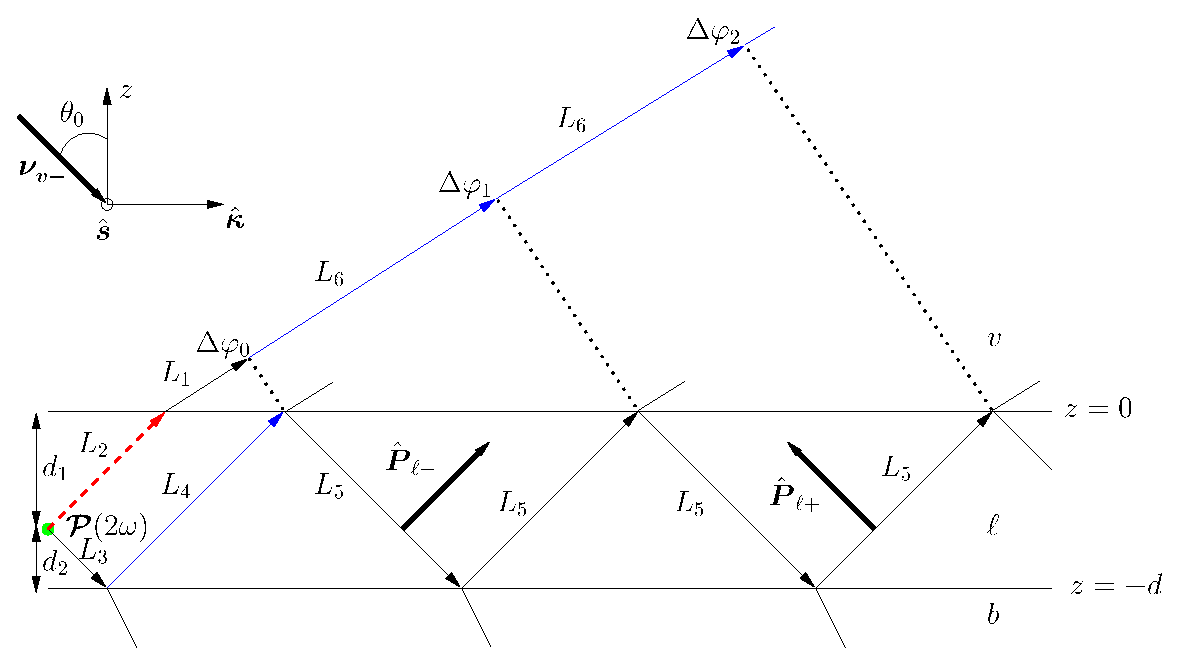
\includegraphics[scale=.5]{figures/multi}
\caption{Sketch of the three layer model for SHG. Vacuum ($v$) is on top with
$\epsilon_v=1$; the layer $\ell$, of thickness $d=d_1+d_2$, is characterized
with $\epsilon_{\ell}(\omega)$, and it is where the SH polarization sheet
$\boldsymbol{\mathcal{P}}(2\omega)$ is located at $z_\ell=d_1$; The bulk $b$ is
described with $\epsilon_{b}(\omega)$. The arrows point along the direction of
propagation, and the $p$-polarization unit vector, $\hat\bfP_{\ell -(+)}$, along
the downward (upward) direction is denoted with a thick arrow. The
$s$-polarization unit vector $\hat\bfs$, points out of the page. The fundamental
field $\bfE(\go)$ is incident from the vacuum side along the
$z\hat{\boldsymbol{\kappa}}$-plane, with $\theta_0$ its angle of incidence and
$\boldsymbol{\nu}_{v-}$ its wave vector. $\Delta\varphi_{i}$ denote the phase
difference of the multiply reflected beams with respect to the first vacuum
transmitted beam (dashed-red arrow), where the dotted lines are perpendicular to
this beam (see the text for details).\label{3layer}}
\end{figure}

To describe the propagation of the SH field, we  see from
Fig. \ref{3layer}, that it is refracted at the 
layer-vacuum interface ($\ell v$), and multiply reflected from the
layer-bulk ($\ell b$)
and layer-vacuum ($\ell v$)
interfaces, thus we can define,
\begin{equation}\label{r5}
\mathbf{T}^{\ell v}
= \hat{\mathbf{s}}T_s^{\ell v}\hat{\mathbf{s}} 
+ \hat{\mathbf{P}}_{v+}T_{p}^{\ell v} \hat{\mathbf{P}}_{\ell +},
\end{equation}
as the tensor for transmission from $\ell v$ interface,
\begin{equation}\label{r6}
\mathbf{R}^{\ell b}
= \hat{\mathbf{s}}R_s^{\ell b}\hat{\mathbf{s}}
+ \hat{\mathbf{P}}_{\ell +}R_{p}^{\ell b} \hat{\mathbf{P}}_{\ell -},
\end{equation} 
as the tensor of reflection from the $\ell b$ interface, 
and
\begin{equation}\label{r6b}
\mathbf{R}^{\ell v}
= \hat{\mathbf{s}}R_s^{\ell v}\hat{\mathbf{s}}
+ \hat{\mathbf{P}}_{\ell -}R_{p}^{\ell v} \hat{\mathbf{P}}_{\ell +},
\end{equation} 
as that of the $\ell v$ interface. 
The Fresnel factors in uppercase letters, $T^{ij}_{s,p}$ and $R^{ij}_{s,p}$,
are evaluated at $2\go$  from the following well known formulas 
\begin{equation}\label{e.f1}
\begin{split}
t_s^{ij}(\omega) &=
\frac{2k_{i}(\omega)}{k_{i}(\omega)+k_{j}(\omega)},
\quad\quad  
t_{p}^{ij}(\omega) =
\frac{2k_{i}(\omega)\sqrt{\epsilon_{i}(\omega)\epsilon_j(\omega)}}
     {k_{i}(\omega)\epsilon_{j}(\omega)+k_{j}(\omega)\epsilon_{i}(\omega)},\\
r_s^{ij}(\omega) &=
\frac{k_{i}(\omega) - k_{j}(\omega)}
     {k_{i}(\omega) + k_{j}(\omega)},
\quad\quad 
r_{p}^{ij}(\omega) =
\frac{k_{i}(\omega)\epsilon_{j}(\omega) - k_{j}\epsilon_{i}(\omega)}
     {k_{i}(\omega)\epsilon_{j}(\omega) + k_{j}(\omega)\epsilon_{i}(\omega)}. 
\end{split}
\end{equation}
From these expressions one can show that,
\begin{align}\label{mf}
1 + r^{\ell b}_{s} &= t^{\ell b}_{s}\nonumber\\
1 + r^{\ell b}_{p}
&= \frac{n_b}{n_\ell}
t^{\ell b}_{p} 
\nonumber\\
1 - r^{\ell b}_{p}
&= \frac{n_\ell}{n_b}
   \frac{w_{b}}{w_{\ell}}t^{\ell b}_{p}\\
t^{\ell v}_{p} &= \frac{w_{\ell}}{w_{v}}t^{v\ell}_{p}\nonumber\\
t^{\ell v}_{s} &= \frac{w_{\ell}}{w_{v}}t^{v\ell}_{s}\nonumber 
.
\end{align}


\subsection{Multiple SH reflections}

The SH field $\bfE(2\go)$ radiated by the SH polarization 
$\boldsymbol{\mathcal{P}}(2\go)$
will radiate directly into vacuum and also into the bulk,
where it will be reflected back at the thin-layer-bulk interface into 
the thin layer again and this beam will be multiple-transmitted and 
reflected as shown in Fig.~\ref{3layer}. 
As the two beams propagate a phase difference will develop between
them, according to
\begin{align}\label{m99}
\gD\varphi_m&=\tilde\gO\Big((L_3+L_4+2mL_5)N_\ell
-\big( L_2N_\ell+(L_1+mL_6)N_v\big)
\Big)
\nonumber\\
&=\gd_0 + m\gd\quad m=0,1,2,\ldots
,
\end{align}
where
\begin{align}\label{m97}
\gd_0=8\pi\left(\frac{d_2}{\lambda_0}\right)\sqrt{n^2_\ell(2\go)-\sin^2\theta_0}
,
\end{align}
\begin{align}\label{m96}
\gd=8\pi\left(\frac{d}{\lambda_0}\right)\sqrt{n^2_\ell(2\go)-\sin^2\theta_0}
,
\end{align}
where $\lambda_0$ is the wavelength of the fundamental field in
vacuum, $d$ the thickness of layer $\ell$ and $d_2$ the distance of
$\boldsymbol{\mathcal{P}}(2\omega)$  
from the $\ell b$ interface 
(see Fig.~\ref{3layer}).
We see that
$\gd_0$ is the phase difference of 
the first and second transmitted beams, and $m\gd$ that of the first 
and  third ($m=1$), fourth ($m=2$), etc. beams (see 
Fig.~\ref{3layer}). 

To take into account the multiple reflections of the generated SH
field in the layer $\ell$, we proceed as follows. We show the algebra
for the $p$-polarized SH field, the $s$-polarized field could be
worked out along the same steps. The multiple-reflected $\bfE_p(2\go)$
field is given by
\begin{equation}\label{m7}
\begin{split}
\mathbf{E}(2\omega) 
&=  
E_{p+}(2\omega)\mathbf{T}^{\ell v}\cdot\hat{\mathbf{P}}_{\ell +}
+ E_{p-}(2\omega)\mathbf{T}^{\ell v}
\cdot\mathbf{R}^{\ell b}\cdot\hat{\mathbf{P}}_{\ell-}e^{i\gD\varphi_0}
+ E_{p-}(2\omega)\mathbf{T}^{\ell v}
\cdot\mathbf{R}^{\ell b}\cdot\mathbf{R}^{\ell v}
\cdot\mathbf{R}^{\ell b}\cdot\hat{\mathbf{P}}_{\ell-}e^{i\gD\varphi_1}
\\
&
+ E_{p-}(2\omega)\mathbf{T}^{\ell v}
\cdot\mathbf{R}^{\ell b}\cdot\mathbf{R}^{\ell v}
\cdot\mathbf{R}^{\ell b}\cdot\mathbf{R}^{\ell v}
\cdot\mathbf{R}^{\ell b}\cdot\hat{\mathbf{P}}_{\ell-}e^{i\gD\varphi_2}
+\cdots 
\\
&= 
E_{p+}(2\omega)\mathbf{T}^{\ell v}\cdot\hat{\mathbf{P}}_{\ell +}
+ E_{p-}(2\omega) \mathbf{T}^{\ell v}
\cdot\sum_{m=0}^\infty  
\big(
\mathbf{R}^{\ell b}\cdot\mathbf{R}^{\ell v} 
e^{i\gd}\Big)^m 
\cdot\mathbf{R}^{\ell b}\cdot\hat{\mathbf{P}}_{\ell-}e^{i\gd_0}
.
\end{split}
\end{equation} 
From Eqs.~\eqref{r5}-\eqref{r6b} is easy to show
that
\begin{align}\label{m1}
\mathbf{T}^{\ell v}\cdot 
\Big(\mathbf{R}^{\ell b}\cdot\mathbf{R}^{\ell v}\Big)^n 
\cdot \mathbf{R}^{\ell b}
&=
\hat{\mathbf{s}}
T^{\ell v}_s\Big(R^{\ell b}_sR^{\ell v}_s\Big)^n 
 R^{\ell b}_s 
\hat{\mathbf{s}}
+
\hat{\mathbf{P}}_{v+}
T^{\ell v}_p\Big(R^{\ell b}_pR^{\ell v}_p\Big)^n 
 R^{\ell b}_p 
\hat{\mathbf{P}}_{\ell-}
,
\end{align}
then,
\begin{equation}\label{m7}
\begin{split}
\mathbf{E}(2\omega) 
&= 
\hat{\mathbf{P}}_{\ell +}T^{\ell v}_p
\Big(
E_{p+}(2\omega) 
+
\frac{R^{\ell b}_pe^{i\gd_0}}{1+R^{v\ell}_pR^{\ell b}_pe^{i\gd}}
E_{p-}(2\omega) 
\Big)
,
\end{split}
\end{equation}
where we used $R^{ij}_{s,p}=-R^{ji}_{s,p}$.
Using Eq.~\eqref{r2}, we can readily write
\begin{equation}\label{mr8}
\mathbf{E}(2\omega) = \frac{\gamma i\tilde{\Omega}}{W_{\ell}}
\mathbf{H}_{\ell}\cdot\boldsymbol{\mathcal{P}}(2\omega),
\end{equation}
where
\begin{equation}\label{mr9}
\mathbf{H}_{\ell}
= \hat{\mathbf{s}}\,T_s^{\ell v}
\left(1+
R^M_s
\right)
\hat{\mathbf{s}}
+ \hat{\mathbf{P}}_{v+}T_{p}^{\ell v}
\left(
\hat{\mathbf{P}}_{\ell +} +
R^M_p
 \hat{\mathbf{P}}_{\ell -}
\right). 
\end{equation}
and
\begin{align}\label{m61}
R^M_l\equiv\frac{R^{\ell b}_le^{i\gd_0}}{1+R^{v\ell}_l R^{\ell b}_l e^{i\gd}}
\quad l=s,p
,
\end{align}
is defined as the multiple  ($M$) reflection coefficient.
To make touch with the work of Ref. \cite{mizrahiJOSA88} where
$\boldsymbol{\mathcal{P}}(2\omega)$ is located on top of the
vacuum-surface interface and only the vacuum radiated beam and the
first (and only) reflected beam need to be considered, we take
$\ell=v$ and $d_2=0$, then 
$T^{\ell v}=1$, $R^{v\ell}=0$ and $\gd_0=0$, with which
$R^M_l=R^{vb}_l$. 
Thus, Eq.~\eqref{mr9} coincides with Eq. (3.8) of
Ref. \cite{mizrahiJOSA88}. 

\subsection{Multiple reflections for the linear field}
\begin{figure}[t]
\centering 
\includegraphics[scale=.5]{figures/linear-field}
\caption{(color on line) Sketch for the multiple reflected  fundamental field
$\bfE(\go)$, which impinges from the vacuum side along the
$z\hat{\boldsymbol{\kappa}}$-plane, with $\theta_0$ and $\boldsymbol{\nu}_{v-}$
its angle of incidence and wave vector, respectively. The arrows point along the
direction of propagation. The $p$-polarization unit vectors, $\hat\bfp_{\beta
\pm}$, along the downward (-) or upward (+) direction are denoted with thick
arrows, where $\beta=v$ or $\ell$. The $s$-polarization unit vector $\hat\bfs$
points out of the page, and $(1,2,3,\dots)\phi$ denotes the phase difference for
the multiply reflected beams with respect to the incident field, where the
dotted line is perpendicular to this beam (see the text for
details).\label{linear}}
\end{figure}

Similar to the SH field, here we consider the multiple reflections of
the fundamental field $\bfE(\go)$ inside the thin $\ell$ layer.
In Fig.~\ref{linear} we show the situation where $\bfE(\go)$
impinges from the vacuum side with an angle of incidence $\theta_0$. 
As the first transmitted beam is multiply reflected from the $\ell b$ and the
$\ell v$ interfaces, it accumulates a phase difference of $n\phi$,
with $n=1,2,3,\ldots$, given by
\begin{align}\label{mphi}
\phi&=\frac{\go}{c}(2L_1n_\ell-L_2n_v)
\nonumber\\
&=4\pi\left(\frac{d}{\lambda_0}\right)\sqrt{n^2_\ell-\sin^2\theta_0}
,
\end{align}
where $n_v=1$. Besides the equivalent of Eqs.~\eqref{r6} and
\eqref{r6b}, for $\go$, we also need
\begin{align}\label{mvv}
\mathbf{t}^{v\ell}
= \hat{\mathbf{s}}t_s^{v\ell}\hat{\mathbf{s}} 
+ \hat{\mathbf{p}}_{\ell -}t_{p}^{v\ell} \hat{\mathbf{p}}_{v -}
,
\end{align}
to write
\begin{align}\label{mcvew}
\bfE(\go)
&=E_0\Big[
\bft^{v\ell}
+
\bfr^{\ell b}\cdot\bft^{v\ell}e^{i\phi}
+
\bfr^{\ell b}\cdot\bfr^{\ell v}\cdot \bfr^{\ell b}\cdot\bft^{v\ell} e^{i2\phi}
+
\bfr^{\ell b}\cdot\bfr^{\ell v}\cdot 
\bfr^{\ell b}\cdot\bfr^{\ell v}
\cdot \bfr^{\ell b}\cdot\bft^{v\ell} e^{i3\phi}
+\cdots\Big]\cdot\bfe^{\mathrm{in}}
\nonumber\\
&=E_0\Big[
1
+
\Big(1+
\bfr^{\ell b}\cdot\bfr^{\ell v}e^{i\phi}
+
(\bfr^{\ell b}\cdot\bfr^{\ell v})^2e^{i2\phi}+\cdots
\Big)\cdot
\bfr^{\ell b}e^{i\phi}
\Big]\cdot \bft^{v\ell}\cdot\bfe^{\mathrm{in}}
\nonumber\\
&=
E_0\Big[\hat\bfs t^{v\ell}_s(1+r^M_s)\hat\bfs
+
t^{v\ell}_p\left(\hat\bfp_{\ell-}+\hat\bfp_{\ell+}r^{M}_p
\right)\hat\bfp_{v-}
\Big]\cdot\bfe^{\mathrm{in}}
\end{align}
where
\begin{align}\label{mvrm}
r^M_l=\frac{r^{\ell b}_le^{i\phi}}{1+r^{v\ell}_lr^{\ell
  b}_le^{i\phi}}\quad l=s,p
.
\end{align}
We define $\bfE^l(\go)\equiv E_0\bfe^{\go,l}_\ell$ ($l=s,p$),
where using Eq.~\eqref{r4}, we obtain that
\begin{eqnarray}\label{mcvep}
\bfe^{\go,p}_\ell=\frac{t^{v\ell}_p}{n_\ell}\left( 
r^{M+}_p\sin\theta_0\hat\bfz  
+ 
r^{M-}_pw_\ell\hat{\boldsymbol{\kappa}}
\right)  
,
\end{eqnarray} 
for $p$-input polarization, i.e. $\bfe^{\mathrm{in}}=\hat\bfp_{v-}$, 
and
\begin{eqnarray}\label{mcvep}
\bfe^{\go,s}_\ell=t^{v\ell}_sr^{M+}_s\hat\bfs
,
\end{eqnarray}
for $s$-input polarization, i.e. $\bfe^{\mathrm{in}}=\hat\bfs$,
where
\begin{eqnarray}\label{mvc}
r^{M\pm}_l=1\pm r^M \quad l=s,p.
\end{eqnarray}
\subsection{SHG Yield}

The magnitude of the radiated field is given by
$E(2\omega)=\hat{\mathbf{e}}^{\mathrm{out}}\cdot\mathbf{E}(2\omega)$, where
$\hat{\mathbf{e}}^{\mathrm{out}}$ is the polarization vector of the radiated
field, for instance $\hat{\mathbf{s}}$ or $\hat{\mathbf{P}}_{v+}$. Then, we
write
\begin{equation}\label{m1}
\begin{split}
\hat{\mathbf{P}}_{\ell +} + R^M_p\hat{\mathbf{P}}_{\ell -}
&= \frac{\sin\theta_0\hat{\mathbf{z}} - W_{\ell}\hat{\boldsymbol{\kappa}}}
        {N_{\ell}}
 + R^M_p
   \frac{\sin\theta_0\hat{\mathbf{z}} + W_{\ell}\hat{\boldsymbol{\kappa}}}
        {N_{\ell}}
\\
&= \frac{1}{N_{\ell}}
\left(
\sin\theta_0R^M_{p+}\hat{\mathbf{z}}
- K_{\ell}R^M_{p-}\hat{\boldsymbol{\kappa}}
\right)
,
\end{split}
\end{equation}
where
\begin{align}\label{rm}
R^{M\pm}_l\equiv 1 \pm R^M_l \quad l=s,p
.
\end{align}
 Using Eq.~\eqref{mf}
 we write Eq.~\eqref{mr8} as
\begin{equation}\label{r10}
E(2\omega) = \frac{2\gamma i \omega}{cW_\ell}
\hat{\mathbf{e}}^{\mathrm{out}}\cdot 
\mathbf{H}_{\ell}\cdot 
\boldsymbol{\mathcal{P}}(2\omega) 
= \frac{2\gamma i \omega}{cW_v}
 \mathbf{e}^{\,2\omega}_{\ell}\cdot\boldsymbol{\mathcal{P}}(2\omega). 
\end{equation}
\begin{equation}\label{r12mm}
\begin{split}
\mathbf{e}^{2\omega}_{\ell} &=\hat{\mathbf{e}}^{\mathrm{out}}\cdot 
\Bigg[
\hat{\mathbf{s}}T_{s}^{v\ell}R^{M+}_s\hat{\mathbf{s}} + 
\hat{\mathbf{P}}_{v+}
\frac{T^{v\ell}_{p}}
     {N_\ell}
\left(
\sin\theta_0R^{M+}_p\hat{\mathbf{z}}
- W_{\ell}R^{M-}_p\hat{\boldsymbol{\kappa}}
\right) 
\Bigg]
. 
\end{split}
\end{equation}  
 We pause here to reduce above result to the case where the nonlinear
polarization $\mathbf{P}(2\omega)$ radiates from vacuum instead from the layer
$\ell$. For such case we simply take $\epsilon_{\ell}(2\omega)=1$ and $\ell=v$
($T^{\ell v}_{s,p}=1$), to get
\begin{equation}\label{r13}
\mathbf{e}^{\,2\omega}_{v} = \hat{\mathbf{e}}^{\mathrm{out}}
\cdot\left[
\hat{\mathbf{s}}T_s^{v b}\hat{\mathbf{s}} + \hat{\mathbf{P}}_{v+}
\frac{T^{v b}_{p}}{\sqrt{\epsilon_{b}(2\omega)}}
\left(
  \epsilon_{b}(2\omega)\sin\theta_0\hat{\mathbf{z}}
  - W_{b}\hat{\boldsymbol{\kappa}}
\right) 
\right] 
,
\end{equation}
which agrees with Eq. (3.10) of Ref. \cite{mizrahiJOSA88}.

In the three layer model the SH polarization $\calbp(2\go)$ is located in layer $\ell$,
where we evaluate the fundamental field required in Eq. \eqref{tres}.
We write
\begin{equation}\label{m2}
\mathbf{E}_{\ell}(\omega)=E_0\left(
\hat{\mathbf{s}} t^{v\ell}_s(1+r^{\ell b}_s)\hat{\mathbf{s}}
+
\hat{\mathbf{p}}_{\ell-}
 t^{v\ell}_{p}
\hat{\mathbf{p}}_{v-}
+
\hat{\mathbf{p}}_{\ell+}
t^{v\ell}_{p}r^{\ell b}_{p}
\hat{\mathbf{p}}_{v-}
\right)\cdot\hat{\mathbf{e}}^{\mathrm{in}}=E_0\mathbf{e}^\omega_{\ell}
,
\end{equation} 
where $\bfe^{\mathrm{in}}$ is the $s$ ($\hat\bfs$) or $p$
($\hat\bfp_{v-}$)
incoming polarization of
the fundamental electric field. 
Above field is composed of the transmitted field and its first
reflection from the $\ell b$ interface for $s$ and $p$ polarizations.
The fundamental field, once inside the layer $\ell$ will be multiply
reflected at the $\ell v$ and $\ell b$ interfaces, however each
reflection will diminish the intensity of the fundamental field, and as the SHG
yield goes with the square of this field, the contribution of the
subsequent reflections, other than the one considered in
Eq.~\eqref{m2},  could be safely neglected.
From Eq.~\eqref{mf}
we find that
\begin{equation}\label{m12}
\mathbf{e}^{\omega}_{\ell}
= \left[
\hat{\mathbf{s}}t_{s}^{v\ell}t_{s}^{\ell b}\hat{\mathbf{s}} 
+ \frac{t^{v\ell}_{p}t^{\ell b}_{p}}
       {n^2_\ell n_b}
\left(
  n^2_b
\sin\theta_0\hat{\mathbf{z}}
+ n^2_\ell w_b\hat{\boldsymbol{\kappa}}
\right)
\hat{\mathbf{p}}_{v-}
\right]
\cdot\hat{\mathbf{e}}^{\mathrm{in}}.  
\end{equation}  
Again, to touch base with Ref. \cite{mizrahiJOSA88},
if we would like to evaluate the fields in the bulk, instead of the layer
$\ell$, we simply take 
$n_\ell=n_b,\,(t^{\ell b}_{s,p}=1$), to obtain
\begin{equation}\label{m13}
\mathbf{e}^{\omega}_{b}
= \left[
\hat{\mathbf{s}}t_{s}^{vb}\hat{\mathbf{s}}
+ \frac{t^{vb}_{p}}{n_b}
\left(
\sin\theta_0\hat{\mathbf{z}} + w_b\hat{\boldsymbol{\kappa}}
\right) 
\hat{\mathbf{p}}_{v-}
\right]
\cdot\hat{\mathbf{e}}^{\mathrm{in}},  
\end{equation} 
that is in agreement with Eq. (3.5) of Ref. \cite{mizrahiJOSA88}.
Then,
 we can write Eq. \eqref{tres} as
\begin{equation}\label{m4}
\boldsymbol{\mathcal{P}}(2\omega) = 
\left\{
\begin{array}{cc}  
E^{2}_{0}\,\boldsymbol{\chi}:\mathbf{e}^{\omega}_{\ell}\mathbf{e}^{\omega}_{\ell}
& \text{(cgs units)} \\
\ge_0E^{2}_{0}\,\boldsymbol{\chi}:\mathbf{e}^{\omega}_{\ell}\mathbf{e}^{\omega}_{\ell}
& \text{(MKS units)} \\
\end{array}
\right.
,
\end{equation}
where $E_0$ is the intensity of the fundamental electric field.
Finally, with above equation we write Eq.~\eqref{r10} as
\begin{equation}\label{mr10}
E(2\omega) 
= \frac{2\eta i \omega}{cW_v}
\mathbf{e}^{2\omega}_{\ell}\cdot\boldsymbol{\chi}:\mathbf{e}^{\omega}_{\ell}
\mathbf{e}^{\omega}_{\ell}
,
\end{equation}
where $\eta=2\pi$ for cgs units and $\eta=1/2$ for MKS units.
To ease on the notation, we define
\begin{align}\label{mc0}
\Upsilon_{\mathrm{iO}}
\equiv 
\mathbf{e}^{2\omega}_{\ell}\cdot\boldsymbol{\chi}:\mathbf{e}^{\omega}_{\ell}
\mathbf{e}^{\omega}_{\ell}
,
\end{align}
where i stands for the incoming polarization of the fundamental
electric field given by $\hat\bfe^{\mathrm{in}}$ in Eq.~\eqref{m12},
and O for the outgoing polarization of the SH electric field
given by $\hat\bfe^{\mathrm{out}}$ in Eq.~\eqref{r12mm}.

From Eqs. \eqref{uno} and \eqref{dos} we obtain that
in the cgs units ($\eta=2\pi$)
\begin{align}\label{r01}
|E(2\omega)|^2 
&= |E_{0}|^4\frac{16\pi^{2}\omega^{2}}{c^{2}W^2_v}
\left\vert  
\Upsilon_{\mathrm{iO}}
\right\vert^{2}
\nonumber\\
\frac{c}{2\pi}|\sqrt{N_v}E(2\omega)|^{2} 
&=
\frac{32\pi^{3}\omega^{2}}{c^{3}\cos^2\theta_0}
\left\vert  
\frac{\sqrt{N_v}}{n^2_\ell}
\Upsilon_{\mathrm{iO}}
\right\vert^{2} 
\left(\frac{c}{2\pi}|\sqrt{n_\ell}E_{0}|^{2}\right)^{2},
\nonumber\\ 
I(2\omega) 
&= \frac{32\pi^{3}\omega^{2}}{c^{3}\cos^2\theta_0}
\left\vert  
\frac{\sqrt{N_v}}{n^2_\ell}
\Upsilon_{\mathrm{iO}}
\right\vert^{2}I^{2}(\omega),
\nonumber\\
\calr_{\mathrm{iO}}(2\omega) 
&= 
\frac{32\pi^{3}\omega^{2}}{c^{3}\cos^2\theta_0}
\left\vert  
\frac{1}{n_\ell}
\Upsilon_{\mathrm{iO}}
\right\vert^{2}
,
\end{align} 
and in MKS units ($\eta=1/2$)
\begin{align}\label{r01m}
|E(2\omega)|^2 
&= |E_{0}|^4
\frac{\omega^{2}}{c^{2}W^2_v}
\left\vert  
\Upsilon_{\mathrm{iO}}
\right\vert^{2}
\nonumber\\
2\ge_0c|\sqrt{N_v}E(2\omega)|^{2} 
&=
\frac{2\ge_0\omega^{2}}{c\cos^2\theta_0}
\left\vert  
\frac{\sqrt{N_v}}{n^2_\ell}
\Upsilon_{\mathrm{iO}}
\right\vert^{2} 
\frac{1}{4\ge^2_0c^2}\left(2\ge_0c|\sqrt{n_\ell}E_{0}|^{2}\right)^{2},
\nonumber\\ 
I(2\omega) 
&= 
\frac{\omega^{2}}{2\ge_0c^3\cos^2\theta_0}
\left\vert  
\frac{\sqrt{N_v}}{n^2_\ell}
\Upsilon_{\mathrm{iO}}
\right\vert^{2}I^{2}(\omega),
\nonumber\\
\calr_{\mathrm{iO}}(2\omega) 
&= \frac{\omega^{2}}{2\ge_0c^3\cos^2\theta_0}
\left\vert  
\frac{1}{n_\ell}
\Upsilon_{\mathrm{iO}}
\right\vert^{2} 
,
\end{align} 
\begin{equation}\label{mc6}
\calr_{\mathrm{iO}}(2\omega) 
\left\{
\begin{array}{cc} 
\frac{32\pi^{3}\omega^{2}}{c^{3}\cos^2\theta_0}
\left\vert  
\frac{1}{n_\ell}
\Upsilon_{\mathrm{iO}}
\right\vert^{2} 
& \text{(cgs units)} \\
\frac{\omega^{2}}{2\ge_0c^3\cos^2\theta_0}
\left\vert  
\frac{1}{n_\ell}
\Upsilon_{\mathrm{iO}}
\right\vert^{2} 
& \text{(MKS units)} 
\end{array}
\right.
,
\end{equation}
as the SHG yield, where $N_v=1$ and $W_v=\cos\theta_0$.
In the MKS unit system $\boldsymbol{\chi}$ is given in m$^2$/V, since
it is a surface second order nonlinear susceptibility, and
$\calr_{\mathrm{iO}}$ is given in m$^2$/W. 


\verb=tal vez esto al apendice=
At this point we mention that to recover the results of Ref.
\cite{mizrahiJOSA88} which are equivalent of those of Ref. \cite{sipePRB87}, we
take $\mathbf{e}^{2\omega}_{\ell}\to \mathbf{e}^{2\omega}_v$,
$\mathbf{e}^{\omega}_{\ell}\to \mathbf{e}^{\omega}_{b}$, 
and then
\begin{equation}\label{m69}
\calr(2\omega) =
\frac{32\pi^{3} \omega^{2}}{c^{3}\cos^{2}\theta_0}
\left\vert
\mathbf{e}^{\,2\omega}_{v}\cdot\boldsymbol{\chi}:
\mathbf{e}^{\omega}_{b}\mathbf{e}^{\omega}_{b}
\right\vert^{2} 
,
\end{equation}
will give the SHG yield of a nonlinear polarization sheet radiating from vacuum
on top of the surface and where the fundamental field is evaluated below the
surface that is characterized by $\epsilon_{b}(\omega)$.


\section{One SH Reflection}
Therefore, the total radiated field at 
$2\omega$ is 
\begin{equation}\label{r7}
\begin{split}
\mathbf{E}(2\omega)  
&= E_s(2\omega)  
\left(
\mathbf{T}^{\ell v} + \mathbf{T}^{\ell v}\cdot\mathbf{R}^{\ell b}
\right)  
\cdot\hat{\mathbf{s}}\nonumber\\
&+ E_{p+}(2\omega)\mathbf{T}^{\ell v}\cdot\hat{\mathbf{P}}_{\ell +}
 + E_{p-}(2\omega)\mathbf{T}^{\ell v}
\cdot\mathbf{R}^{\ell b}\cdot\hat{\mathbf{P}}_{\ell-}.  
\end{split}
\end{equation} 
The first term is  the transmitted $s$-polarized field, the second one is the 
reflected and then transmitted $s$-polarized field and the third and fourth 
terms are the equivalent fields for $p$-polarization. The transmission is from 
the layer into vacuum, and the reflection between the layer and the bulk. After 
some simple algebra, we obtain 
\begin{equation}\label{r8}
\mathbf{E}(2\omega) = \frac{2\pi i\tilde{\Omega}}{K_{\ell}}
\mathbf{H}_{\ell}\cdot\boldsymbol{\mathcal{P}}(2\omega),
\end{equation} 
where,
\begin{equation}\label{r9}
\mathbf{H}_{\ell}
= \hat{\mathbf{s}}\,T_s^{\ell v}\left(1+R_s^{\ell b}\right)\hat{\mathbf{s}}
+ \hat{\mathbf{P}}_{v+}T_{p}^{\ell v}
\left(
\hat{\mathbf{P}}_{\ell +} +R_{p}^{\ell b}\hat{\mathbf{P}}_{\ell -}
\right). 
\end{equation}

%%%%%%%%%%%%%%%%%%%%%%%%%%%%%%%%%%%%%%%%%%%%%%%%%%%%%%%%%%%%%%%%
%%%%%%%%%%%%%%%%%%%%%%%%%%%%%%%%%%%%%%%%%%%%%%%%%%%%%%%%%%%%%%%%
%%%%%%%%%%%%%%%%%%%%%%%%%%%%%%%%%%%%%%%%%%%%%%%%%%%%%%%%%%%%%%%%

\section{\texorpdfstring{$\mathcal{R}$}{R} for different polarization cases}

\subsection{\texorpdfstring{$\mathcal{R}_{pP}$}{RpP}}

We develop five different scenarios for $\mathcal{R}_{pP}$ that explore
different cases for where the polarization and fundamental fields are located.
In all these scenarios, we use
$\hat{\mathbf{e}}^{\mathrm{in}}=\hat{\mathbf{p}}_{v-}$ in Eq. \eqref{m12}, and
$\hat{\mathbf{e}}^{\mathrm{out}}=\hat{\mathbf{P}}_{v+}$ in Eq.
\eqref{r12}.

This scenario involves $\mathcal{P}(2\omega)$ and the fundamental fields to be
taken in a thin layer of material below the surface, which we designate as
$\ell$. Thus,
\begin{equation*}\label{m80}
\mathbf{e}^{\,2\omega}_{\ell}\cdot\boldsymbol{\chi}:
\mathbf{e}^\omega_{\ell}\mathbf{e}^\omega_{\ell}
\equiv\Gamma^{\ell}_{pP}\,r^{\ell}_{pP}
,
\end{equation*}
where
\begin{align}\label{m81}
r^{\ell}_{pP} &=
\epsilon_{b}(2\omega)\sin\theta_{\mathrm{in}}
\Big(
  \epsilon^2_{b}(\omega)\sin^2\theta_{\mathrm{in}}\chi_{zzz}
+ \epsilon^2_{\ell}(\omega)k^2_{b}\chi_{zxx}
\Big)\\
&- \epsilon_{\ell}(2\omega)\epsilon_{\ell}(\omega)k_{b}K_{b}
\Big(
  2\epsilon_{b}(\omega)\sin\theta_{\mathrm{in}}\chi_{xxz}
+ \epsilon_{\ell}(\omega)k_{b}\chi_{xxx}\cos(3\phi) 
\Big),\nonumber
\end{align}
and  
\begin{equation}\label{m79}
\Gamma^{\ell}_{pP}=
\frac{T_{p}^{\ell v}T^{\ell b}_{p}}
     {\epsilon_{\ell}(2\omega)\sqrt{\epsilon_{b}(2\omega)}}
\left(
\frac{t_{p}^{v\ell}t^{\ell b}_{p}}
     {\epsilon_{\ell}(\omega)\sqrt{\epsilon_{b}(\omega)}}
\right)^{2} 
.  
\end{equation}


\subsection{\texorpdfstring{$\mathcal{R}_{pS}$}{RpS}}

To obtain $R_{pS}(2\omega)$ we use
$\hat{\mathbf{e}}^{\mathrm{in}}=\hat{\mathbf{p}}_{v-}$ in Eq. \eqref{m12}, and
$\hat{\mathbf{e}}^{\mathrm{out}}=\hat{\mathbf{S}}$ in Eq. \eqref{r12}. We also
use the unit vectors defined in Eqs. \eqref{eq:kappavec} and
\eqref{eq:svec}. Substituting, we get
\begin{equation*}
\mathbf{e}^{\,2\omega}_{\ell}\cdot
\boldsymbol{\chi}:\mathbf{e}^\omega_{\ell}\mathbf{e}^\omega_{\ell}
\equiv\Gamma^{\ell}_{sP}\, r^{\ell}_{sP},
\end{equation*}
where
\begin{equation}
r^{\ell}_{pS}
= -\epsilon^{2}_{\ell}(\omega)k^{2}_{b}\sin3\phi\chi_{xxx},
\end{equation} 
and  
\begin{equation}
\Gamma^{\ell}_{pS} =
T^{v\ell}_{s}T^{\ell b}_{s}\left(\frac{t^{v\ell}_{p}t^{\ell b}_{p}}
      {\epsilon_{\ell}(\omega)\sqrt{\epsilon_{b}(\omega)}}\right)^{2}.
\end{equation} 
In order to reduce above result to that of Ref. \cite{mizrahiJOSA88} and
\cite{sipePRB87},  we take the $2\omega$ radiations factors for vacuum by
taking $\ell=v$, thus $\epsilon_{\ell}(2\omega)=1$, $T^{v\ell}_{s}=1$,
$T^{\ell b}_{s}=T^{vb}_{s}$, and the fundamental field inside medium $b$ by
taking $\ell=b$, thus $\epsilon_{\ell}(\omega)=\epsilon_{b}(\omega)$,
$t^{v\ell}_{p}=t^{vb}_{p}$, and $t^{\ell b}_{p}=1$. With these choices,
\begin{equation*}
r^{b}_{pS} = -k^{2}_{b}\sin3\phi\chi_{xxx},
\end{equation*} 
and 
\begin{equation*}
\Gamma^{b}_{pS} =
T^{vb}_{s}
\left(
\frac{t^{vb}_{p}}{\sqrt{\epsilon_{b}(\omega)}}
\right)^{2}.  
\end{equation*} 


\subsection{\texorpdfstring{$\mathcal{R}_{sP}$}{RsP}}

To obtain $R_{sP}(2\omega)$ we use
$\hat{\mathbf{e}}^{\mathrm{in}}=\hat{\mathbf{s}}$ in Eq. \eqref{m12}, and
$\hat{\mathbf{e}}^{\mathrm{out}}=\hat{\mathbf{P}}_{v+}$ in Eq. \eqref{r12}. We
also use the unit vectors defined in Eqs. \eqref{eq:kappavec} and
\eqref{eq:svec}. Substituting, we get
\begin{equation*}
\mathbf{e}^{\,2\omega}_{\ell}\cdot
\boldsymbol{\chi}:\mathbf{e}^\omega_{\ell}\mathbf{e}^\omega_{\ell}
\equiv\Gamma^{\ell}_{sP}\, r^{\ell}_{sP},
\end{equation*}
where
\begin{equation}
r^{\ell}_{sP}
= \epsilon_{b}(2\omega)\sin\theta_{\mathrm{in}}\chi_{zxx}
+ \epsilon_{\ell}(2\omega)K_{b}\chi_{xxx}\cos3\phi,
\end{equation} 
and  
\begin{equation}
\Gamma^{\ell}_{sP}=
\frac{T_{p}^{\ell v}T^{\ell b}_{p}\left(t_s^{v\ell}t^{\ell b}_s\right)^2}
     {\epsilon_{\ell}(2\omega)\sqrt{\epsilon_{b}(2\omega)}}.  
\end{equation} 
In order to reduce above result to that of Ref. \cite{mizrahiJOSA88} and
\cite{sipePRB87}, we take the $2\omega$ radiations factors for vacuum by
taking $\ell=v$, thus $\epsilon_{\ell}(2\omega)=1$, $T^{v\ell}_{p}=1$,
$T^{\ell b}_{p}=T^{vb}_{p}$, and the fundamental field inside medium $b$ by
taking $\ell=b$, thus $\epsilon_{\ell}(\omega)=\epsilon_{b}(\omega)$,
$t^{v\ell}_s=t^{vb}_s$, and $t^{\ell b}_s=1$. With these choices,
\begin{equation*}
r^{b}_{sP} = \epsilon_{b}(2\omega)\sin\theta_{\mathrm{in}}\chi_{zxx}
+ K_{b}\chi_{xxx}\cos3\phi,
\end{equation*} 
and 
\begin{equation*}
\Gamma^{b}_{sP} =
\frac{T^{v b}_{p}(t_s^{vb})^{2}}{\sqrt{\epsilon_{b}(2\omega)}}.  
\end{equation*}


\subsection{\texorpdfstring{$\mathcal{R}_{sS}$}{RsS}}

For $\mathcal{R}_{sS}$ we have that
$\hat{\mathbf{e}}^{\mathrm{in}}=\hat{\mathbf{s}}$ and
$\hat{\mathbf{e}}^{\mathrm{out}}=\hat{\mathbf{S}}$. This leads to
\begin{equation*}
\mathbf{e}^{\,2\omega}_{\ell}\cdot
\boldsymbol{\chi}:\mathbf{e}^\omega_{\ell}\mathbf{e}^\omega_{\ell}
\equiv\Gamma^{\ell}_{sS}\, r^{\ell}_{sS},
\end{equation*}
where
\begin{equation}
r^{\ell}_{sS} = \chi_{xxx}\sin3\phi,
\end{equation}
and
\begin{equation}
\Gamma^{\ell}_{sS}=
T^{v\ell}_{s}T^{\ell b}_{s}\left(t^{v\ell}_{s}t^{\ell b}_{s}\right)^{2}.
\end{equation} 
In order to reduce above result to that of Ref. \cite{mizrahiJOSA88} and
\cite{sipePRB87}, we take the $2\omega$ radiations factors for vacuum by
taking $\ell=v$, thus $\epsilon_{\ell}(2\omega)=1$, $T^{v\ell}_{s}=1$,
$T^{\ell b}_{s}=T^{vb}_{s}$, and the fundamental field inside medium $b$ by
taking $\ell=b$, thus $\epsilon_{\ell}(\omega)=\epsilon_{b}(\omega)$,
$t^{v\ell}_{s}=t^{vb}_{s}$, and $t^{\ell b}_{s}=1$. With these choices,
\begin{equation*}
r^{b}_{sS} = \chi_{xxx}\sin3\phi,
\end{equation*}
and 
\begin{equation*}
\Gamma^{b}_{sS} = T^{vb}_{s}\left(t^{vb}_{s}\right)^{2}.
\end{equation*} 


\subsection{Summary}

We present the final expressions for each polarization case in Table
\ref{tab:summary}.

\begin{table}[t]
\centering
\begin{tabular}{ | c | p{80pt} | p{210pt} | }
\hline
$iF$ & $\Gamma^{\ell}_{iF}$ & $r^{\ell}_{iF}$ \\
\hline
&&\\
$pP$ &
$\frac{T^{v\ell}_{p}}{N_{\ell}}
\left(\frac{t^{v\ell}_{p}t^{\ell b}_{p}}{n^{2}_{\ell}n_{b}}\right)^{2}$ &
{\small
$R^{M+}_{p}\sin\theta_{0}
(n^{4}_{b}\sin^{2}\theta_{0}\chi_{zzz} + n^{4}_{\ell}w^{2}_{b}\chi_{zxx})
\newline- R^{M-}_{p}n^{2}_{\ell}w_{b}W_{\ell}
(2n^{2}_{b}\sin\theta_{0}\chi_{xxz} + n^{2}_{\ell}w_{b}\chi_{xxx}\cos3\phi)$
}
\\[3pt]
%%%%%%%%%%%%%%%%%%%%%%%%%%%%%%%%%%%%%%%%%%%%%%%%%%%%%%%%%%%%%%%%%%%%%%%
$pS$ &
$T_{s}^{v\ell}R^{M+}_{s}
\left(\frac{t^{v\ell}_{p}t^{\ell b}_{p}}{n^{2}_{\ell}n_{b}}\right)^{2}$ &
$-n^{4}_{\ell}w^{2}_{b}\chi_{xxx}\sin3\phi$
\\[15pt]
%%%%%%%%%%%%%%%%%%%%%%%%%%%%%%%%%%%%%%%%%%%%%%%%%%%%%%%%%%%%%%%%%%%%%%%
$sP$ &
$\frac{T^{v\ell}_{p}}{N_{\ell}}\left(t^{v\ell}_{s}t^{\ell b}_{s}\right)^{2}$ &
$R^{M+}_{p}\sin\theta_{0}\chi_{zxx} + R^{M-}_{p}W_{\ell}\chi_{xxx}\cos3\phi$
\\[15pt]
%%%%%%%%%%%%%%%%%%%%%%%%%%%%%%%%%%%%%%%%%%%%%%%%%%%%%%%%%%%%%%%%%%%%%%%
$sS$ & 
$T_{s}^{v\ell}R^{M+}_{s}\left(t^{v\ell}_{s}t^{\ell b}_{s}\right)^{2}$ &
$\chi_{xxx}\sin3\phi$
\\[15pt]
\hline
\end{tabular}
\caption{The expressions needed to calculate the SHG yield for the (111)
surface, for each polarization case.\label{tab:summary}}
\end{table}

\chapter{Results}\label{chap:results}
%\minitoc

\section{Chi2}

In this section we present a relevant test case to check the consistency of our
approach. We have selected a clean Si(001) surface with a $2\times 1$ surface
reconstruction. The slab for such a surface could be chosen to be
centrosymmetric by creating the front and back surfaces with the same $2\times
1$ reconstruction. However, we choose to terminate one of the surfaces with
hydrogen producing an ideal terminated bulk Si surface. The H atoms simply
saturate the dangling bonds of the bulk-like Si atoms at the surface, as seen in
Fig.~\ref{si2x1}. We take the $z$ coordinate pointing out of the surface and the
$x$ coordinate along the crystallographic [011] direction is parallel to the
dimmers.
\begin{figure}
\centering 
\includegraphics[scale=.8]{figures/03-results/chi2/fig2}
\caption{(color on line) The slab shows a 
clean Si(001)$2\times 1$ front surface with an ideal terminated Si bulk back
surface. The dangling bonds are H (small balls) saturated. This image depicts 12
Si atomic layers with one H atomic layer.
\label{si2x1}} 
\end{figure} 
The idea behind this slab configuration is that the cristalline symmetry of the
H terminated surface imposes that $\chi_{\mathrm{H}}^{xxx}=0$. The $2\times 1$
surface has no such restrictions, so $\chi_{2\times 1}^{xxx}\ne 0$. This is due
to the fact that along the $y$ direction there is a mirror plane for the
H-saturated surface, whereas for the $2\times 1$ surface this mirror is lost as
the dimers are asymmetric along $x$. Thus, calculating $\chi^{xxx}$ for the
full-slab, or the half-slab containing the $2\times 1$ surface\cite{note1}
should yield the same result since the contribution from the H saturated surface
is zero regardless. We must check that the following relationship is satisfied
for this particular slab
\begin{equation*}
\chi_{\mathrm{half-slab}}^{xxx}(-2\omega;\omega,\omega) 
=
\chi_{\mathrm{full-slab}}^{xxx}(-2\omega;\omega,\omega) 
,
\end{equation*}
where $\chi_{\mathrm{half-slab}}^{xxx}(-2\omega;\omega,\omega)$ is calculated
using ${\mathbf{\cal C}}(z)=1$ from the upper half containing the $2\times 1$
surface reconstruction, as seen in Fig.~\ref{si2x1}, and
$\chi_{\mathrm{full-slab}}^{xxx}(-2\omega;\omega,\omega)$ is calculated using
${\mathbf{\cal C}}(z)=1$ through the full slab. We show the results for this
comparison in the remainder of this section. Also, we checked that for the
dihydride surface $\chi_{\mathrm{half-slab}}^{xxx}(-2\omega;\omega,\omega)=0$.

The self-consistent ground state and the Kohn-Sham states were calculated in the
DFT-LDA framework using the plane-wave ABINIT code.\cite{abinit} We used
Troullier-Martins pseudopotentials\cite{troullierPRB91} that are fully separable
nonlocal pseudopotentials in the Kleinman-Bylander form.\cite{kleinmanPRL82} The
contribution of $\mathbf{v}^\mathrm{nl}$ and $\boldsymbol{\mathcal{\cal
V}}^\mathrm{nl}$ to Eq.~\eqref{chis} is carried out using the DP
code.\cite{olevanoDP} The surfaces have been studied with the experimental
lattice constant of 5.43 \AA. Structural optimizations were performed with the
ABINIT code.\cite{abinit} The geometry optimization has been carried out in
slabs of 12 atomic layers where the central four layers where fixed at the bulk
positions. The structures were relaxed until the Cartesian force components were
less than 5 meV/\AA. The geometry optimization for the clean surface gives a
dimer buckling of 0.721 \AA, and a dimer length of 2.301 \AA. For the
Si(001)$1\times 1$:2H dihydride surface, we have obtained a Si-H bond distance
of 1.48 \AA. This results are in good agreement with previous theoretical
studies.\cite{caramellaPRB09,mendozaPRB06} The vacuum size is equivalent to one
quarter the size of the slab, avoiding the effects produced by possible
wave-function tunneling from the contiguous surfaces of the full crystal formed
by the repeated super-cell scheme.\cite{mendozaPRB06}

Spin-orbit, local field, and electron-hole attraction\cite{beyond} effects on
the SHG process are all neglected. Although these are important factors in the
optical response of a semiconductor, their efficient calculation is still
theoretically and numerically challenging and under debate. This merits further
study but is beyond the scope of this paper. For a given slab size, we find the
converged spectra to obtain the relevant parameters. The most important of these
are: an energy cut-off of 10 Ha for the 16, 24, and 32 layered slabs and 13 Ha
for the 40 layer slab, an equal number of conduction and valence bands, and a
set of 244 $\mathbf{k}$-points. The $\mathbf{k}$-points are used for the linear
analytic tetrahedron method for evaluating the 3D Brillouin Zone (BZ) integrals
where special care was taken to examine the double resonances of
Eq.~\eqref{chis}. \cite{nastosPRB05} Note that the Brillouin zone for the slab
geometry collapses to a 2D-zone, with only one $\mathbf{k}$-point along the
$z$-axis. All spectra were calculated with a Gaussian smearing of 0.15 eV.
\begin{figure}
\centering 
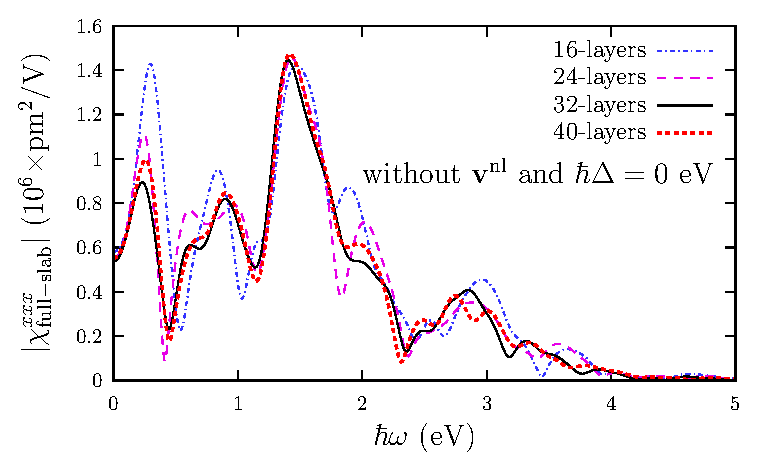
\includegraphics[scale=.8]{figures/03-results/chi2/fig3}
\caption{(color on line) 
$|\chi_{\mathrm{half-slab}}^{xxx}|$ vs $\hbar\omega$ for the slab with 16, 24,
32, and 40 atomic Si layers. The front surface is in a clean $2\times 1$
reconstruction and the back surface is an ideal terminated bulk H-saturated
dangling bonds (see Fig.~\ref{si2x1}).
\label{fig1}} 
\end{figure}
\begin{figure}
\centering 
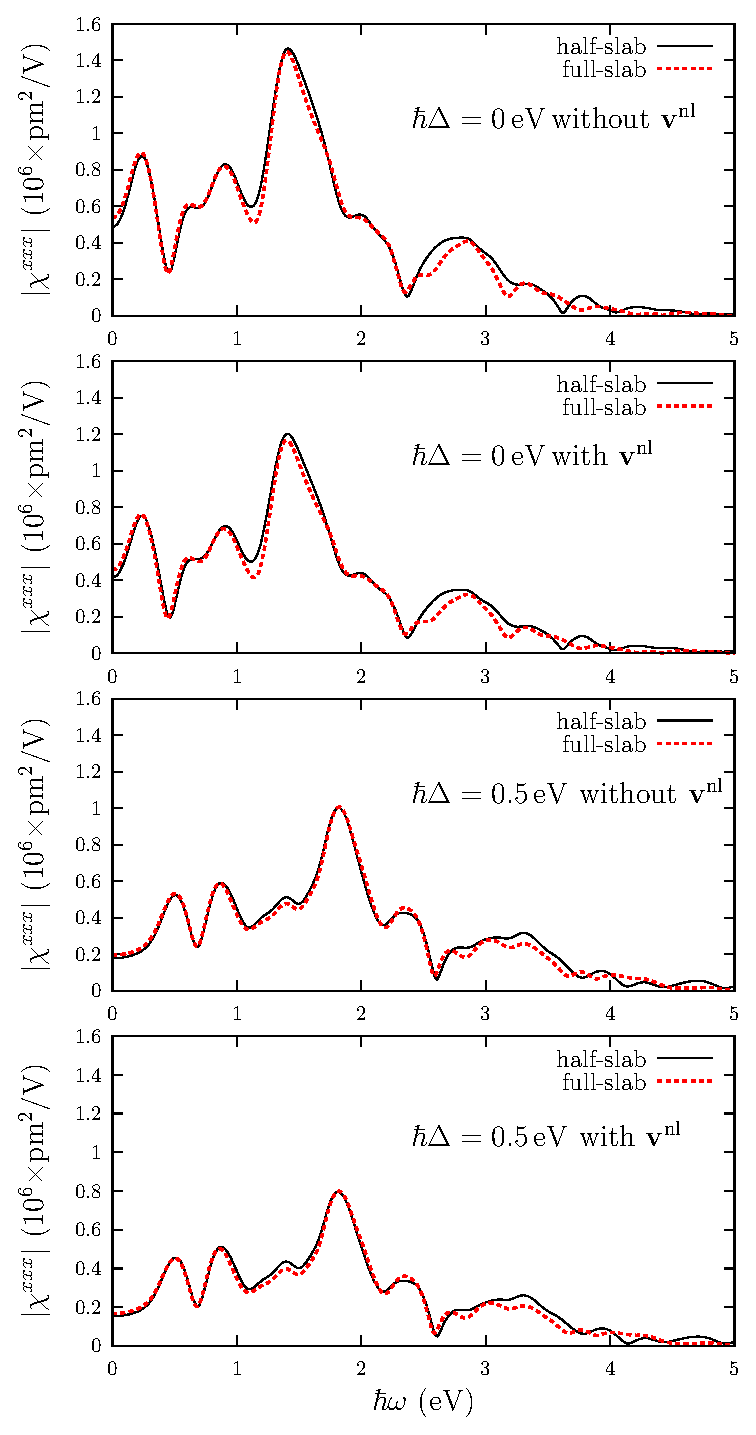
\includegraphics[scale=.8]{figures/03-results/chi2/fig4}
\caption{(color on line) 
$\chi^{xxx}_{\mathrm{half-slab}}$ and $\chi^{xxx}_{\mathrm{full-slab}}$ vs
$\hbar\omega$ for a slab with 32 atomic Si layers plus one H layer.
\label{fig2}} 
\end{figure}

We must evaluate $T^{\mathrm{a}\mathrm{b}}_{nm}=(i/\hbar)[r^\mathrm{b},v^{\mathrm{nl},\mathrm{a}}]_{nm}$ in order to obtain Eqs.~\eqref{tau.1} and
\eqref{tau.1n} that are required for Eq.~\eqref{chis}. Computing second-order
derivatives is required thus making the numerical procedure very time consuming.
This adds significantly to the already lengthy time needed for the calculation
of the $\mathbf{v}^\mathrm{nl}$ contribution that is proportional only to the
first order derivatives. Memory requirements are also increased for both
$\mathbf{v}^\mathrm{nl}$ and $[\mathbf{r},\mathbf{v}^\mathrm{nl}]$. However, the
contribution from $[\mathbf{r},\mathbf{v}^\mathrm{nl}]$ is very
small\cite{valerie} and therefore we neglect it in this work.


\subsection{Full-slab results}\label{fsresults}

In Fig.~\ref{fig1} we show $|\chi_{\mathrm{full-slab}}^{xxx}|$ for the slab with
16, 24, 32, and 40 Si atomic layers, without the contribution of
$\mathbf{v}^{\mathrm{nl}}$ and with no scissors correction. Since the clean
Si(001) surface is $2\times 1$, there are two atoms per atomic layer, thus the
total number of atoms per slab is twice the number of atomic layers of the slab.
In making the slabs larger, we add steps of 8 layers of bulk-like atomic
positions. We note that the response differs substantially for 16 and 24 layers
but is quite similar for 32 and 40 layers. As explained above, the calculation
of the $\mathbf{v}^\mathrm{nl}$ contribution is computationally expensive. A
good compromise between the accuracy in the convergence of
$\chi^{xxx}_{\mathrm{full-slab}}$ as a function of the number of layers in the
slab, and the computational expense is to consider the slab with 32 Si atomic
layers as an accurate representation of our system.


\subsection{Half-slab vs. full-slab}

In Fig.~\ref{fig2} we compare $\chi^{xxx}_{\mathrm{half-slab}}$ vs.
$\chi^{xxx}_{\mathrm{full-slab}}$ for the four different possibilities between
including or not including the effects of $\mathbf{v}^\mathrm{nl}$ or the
scissors correction $\hbar\Delta$. For these results we chose $\hbar\Delta=0.5$
eV, that is the GW gap reported in Refs. \cite{rohlfingPRB95,garciaCPC01}.
This is justified by the fact that the surface states of the clean Si(001)
surface are rigidly shifted and maintain their dispersion relation with respect
to LDA according to the GW calculations of Ref. \cite{rohlfingPRB95}. We
see that for all four instances the difference between responses is quite small.
Indeed, when the value $|\chi^{xxx}|$ is large the difference between the two is
very small; when the value is small the difference increases only slightly, but
the spectra is so close to zero that it is negligible. These differences would
decrease as the number of atomic layers increases. We remark that 32 layers in
the slab is more than enough to confirm that the extraction of the surface
second-harmonic susceptibility from the $2\times 1$ surface is readily possible
using the formalism contained in Eq.~\eqref{chis}. We have confirmed that for
the dihydride surface $|\chi^{xxx}_{\mathrm{half-slab}}|\approx 0$ (not shown).
This confirms the validity of our theory and is the main result of this article;
through the proposed layer formalism we can calculate the surface SH
$\chi^{\mathrm{a}\mathrm{b}\mathrm{c}}(-2\omega;\omega,\omega)$ including the
contribution of the nonlocal part of the pseudopotentials and the part of the
many-body effects through the scissors correction. Our scheme should work for
any slab.

\subsection{\texorpdfstring{Results for $\chi^{xxx}_{2\times 1}(-2\omega;\omega,\omega)$}
{Results for Xxxx(2x1)(-2w;w,w)}}

We proceed to explain some of the features seen in $|\chi^{xxx}_{2\times 1}|$
that, as explained above, are obtained by calculating
$|\chi^{xxx}_{\mathrm{half-slab}}|$. First, from Fig.~\ref{fig2} we note a
series of resonances that derive from 1$\omega$ and 2$\omega$ terms in
Eq.~\eqref{chis}. Notice that the 2$\omega$ resonances start below $E_g/2$ where
$E_g$ is the band gap (0.53 eV  for LDA and 1.03 eV if the scissor is used with
$\hbar\Delta=0.5$ eV). These resonances come from the electronic states of the
$2\times 1$ surface, that lie inside the bulk band gap of Si and are the well
known electronic surface states.\cite{rohlfingPRB95} In Fig.~\ref{fig3} we see
that the effect of $\mathbf{v}^\mathrm{nl}$ reduces the value of
$|\chi^{xxx}_{2\times 1}|$ by 15-20\% showing the importance of this
contribution for a correct calculation of SSHG, in agreement with the analysis
for bulk semiconductors.\cite{luppiPRB08} However, the inclusion of
$\mathbf{v}^\mathrm{nl}$ does not changes the spectral shape of
$|\chi^{xxx}_{2\times 1}|$; this also can be confirmed from the cases of zero
scissors correction from Fig.~\ref{fig2}.
\begin{figure}
\centering 
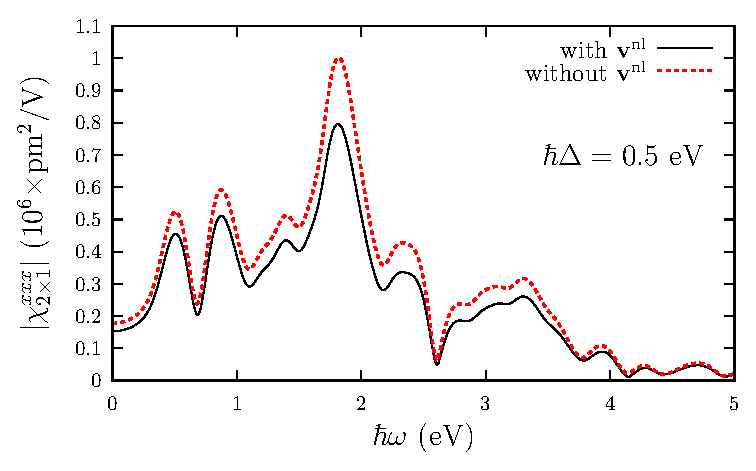
\includegraphics[scale=.8]{figures/03-results/chi2/fig5}
\caption{(color on line) 
$\chi^{xxx}_{2\times 1}$ vs $\hbar\omega$ for a slab with 32 atomic Si layers
plus one H layer, with and without the contribution from
$\mathbf{v}^\mathrm{nl}$.
\label{fig3}} 
\end{figure}

To see the effect of the scissors correction, we take two different finite
values for $\hbar\Delta$. The first one with a value of $\hbar\Delta=0.5$ eV,
used in the above results, is the ``average'' GW gap taken from
Ref. \cite{rohlfingPRB95} that is in agreement with
Ref. \cite{garciaCPC01}. The second one with a value of $\hbar\Delta=0.63$
eV is the ``average'' gap taken from Ref. \cite{asahiPRB00}, where more
$\mathbf{k}$-points in the Brillouin zone were used to calculate its GW value.
From Fig.~\ref{fig4} we note that the scissors correction shifts the spectra
from its LDA value to higher energies as expected. However, contrary to the case
of linear optics\cite{cabellosPRB09} the shift introduced by the scissors
correction is not rigid, as pointed out in Ref. \cite{nastosPRB05}. This
is because the second-harmonic optical response mixes $1\omega$ and $2\omega$
transitions (see Eq.~\eqref{chis}), and accounts for the non-rigid shift. The
reduction of the spectral strength is in agreement with previous calculations
for bulk systems.\cite{nastosPRB05, luppiPRB10, leitsmannPRB05} When we compare
$|\chi^{xxx}_{2\times 1}|$ for the two finite values of $\hbar\Delta$, we see
that the first two peaks are almost rigidly shifted with a small difference in
height while the rest of the peaks are modified substantially. This behavior
comes from the fact that the first two peaks are almost exclusively related to
the 2$\omega$ resonances of Eq.~\eqref{chis}. The other peaks are a combination
of 1$\omega$ and 2$\omega$ resonances and yield a more varied spectrum. We
mention that for large gap materials, the 1$\omega$ and 2$\omega$ would be
splited showing a small interference effect, but still the 2$\omega$ would
strongly depend on the surface states. This way we see that small changes in the
value of the scissors shift can in general affect the SSH susceptibility
spectrum quite dramatically. In Ref. \cite{adolphPRB00}, the authors
already remarked that nonlinear optical response of bulk materials is more
influenced by the electronic structure of the material than the linear case. In
the case of semiconducting surfaces the problem is even more intricate due to
the presence of electronic surface states. The high sensitivity of SSHG to the
energy position  of surface states, as seen in Fig.~\ref{fig4}, makes SSHG a
good benchmark spectroscopical tool for testing the validity of the inclusion of
many-body effects, and in particular the quasi-particle correction to the
electronic states.
\begin{figure}
\centering 
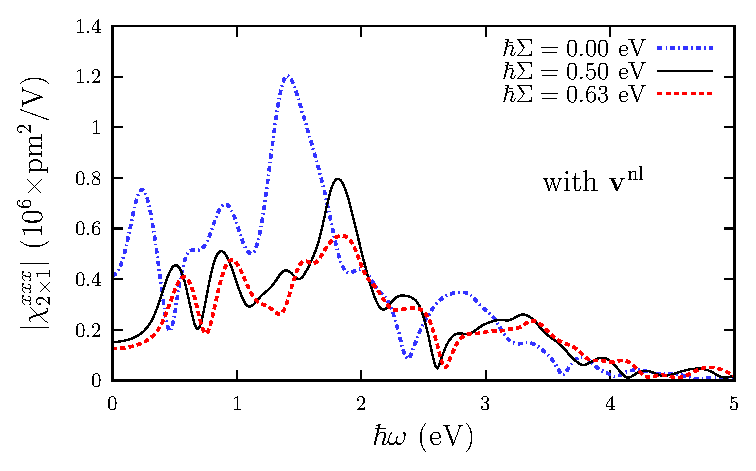
\includegraphics[scale=.8]{figures/03-results/chi2/fig6}
\caption{(color on line) 
$\chi^{xxx}_{2\times 1}$ vs $\hbar\omega$ for a slab with 32 atomic Si layers
plus one H layer, for two different values of the scissors correction
$\hbar\Delta$.
\label{fig4}} 
\end{figure}

Although local fields are neglected they should, in principle, be small parallel
to the interface as the electric field is continuous. So, we would expect that
the $xxx$ component of $\boldsymbol{\chi}(-2\omega;\omega,\omega)$ would have a
small influence from the local fields. Also, the excitonic effects ought to be
explored, but their efficient calculation is theoretically and numerically
challenging\cite{beyond}   and beyond the scope of this article. Unfortunately
the experimental measurement of the $xxx$ component of
$\boldsymbol{\chi}(-2\omega;\omega,\omega)$ is not possible as the SH radiated
intensity would be proportional not only to this component but also to the other
components of $\boldsymbol{\chi}(-2\omega;\omega,\omega)$. However, in a
forthcoming publication we will present a study of SSHG from several Si surfaces
with comparison to experimental results.


\section{SHG Yield}

\section{Method}\label{sec:method}

We constructed the Si(111)(1$\times$1):H surface with the experimental lattice
constant of 5.43 \AA, and then performed structural optimizations with the
ABINIT\cite{gonzeCPS09, abinit} code. The structures were relaxed until the
Cartesian force components were less than 5 meV/\AA, yielding a final Si-H bond
distance of 1.50 \AA. The energy cutoff used was 20 Ha, and we used
Troullier-Martin LDA pseudopotentials.\cite{troullierPRB91} The resulting atomic
positions are in good agreement with previous theoretical studies,
\cite{kaxirasPRB88, jonaPRB95, alfonsoPRB96, cargnoniJOCP00, mejiaPRB02} as well
as the experimental value for the Si-H distance.\cite{weastCRC88}

We also evaluated the number of layers required for convergence and settled on a
slab with 48 atomic Si planes. The geometric optimizations mentioned above are
therefore carried out on slabs of 48 atomic layers without fixing any atoms to
the bulk positions. All of the calculations involve
$\epsilon^{\mathrm{ab}}_{\mathrm{half-slab}}$ and
$\chi^{\mathrm{abc}}_{\mathrm{half-slab}}$, which are calculated with
${\mathbf{\mathcal{C}}}(z)=1$ for the upper half of our slab. This encompasses
24 layers of Si and the single layer of H that terminates the top surface. The
vacuum size is equivalent to one quarter the size of the slab, avoiding the
effects produced by possible wave-function tunneling from the contiguous
surfaces of the full crystal formed by the repeated super-cell
scheme.\cite{mendozaPRB06}

The electronic wave-functions, $\psi_{n\mathbf{k}}(\mathbf{r})$, were also
calculated with the ABINIT code using a planewave basis set with an energy
cutoff of 15 Hartrees. $\chi^{\mathrm{abc}}(-2\omega;\omega,\omega)$ was
properly converged with 576 \textbf{k} points in the irreducible Brillouin zone,
which are equivalent to 1250 \textbf{k} points if we disregard symmetry
relations. The contribution of $\boldsymbol{\mathcal{\cal V}}^\mathrm{nl}$ in
Eq.~\eqref{eq:chis} was carried out using the DP\cite{olevanoDP} code with a
basis set of 3000 planewaves. Convergence for the number of bands was achieved
at 200, which includes 97 occupied bands and 103 unoccupied bands.

All spectra were produced using a scissors value of 0.7\,eV in the
$\chi^{\mathrm{abc}}(-2\omega;\omega,\omega)$ and
$\boldsymbol{\epsilon}_{\ell}(\omega)$ calculations. This value was obtained
from Ref. \cite{liPRB10}, in which the authors carry out a
$\mathrm{G}_{0}\mathrm{W}_{0}$ calculation on this surface for increasing
numbers of layers. They calculated the LDA and $\mathrm{G}_{0}\mathrm{W}_{0}$
band gaps, and found that the difference between the two tends towards
$\sim0.7$\,eV as more layers are added, culminating in a value of 0.68\,eV for
bulk Si. This calculation is completely \emph{ab-initio}, so we choose 0.7\,eV
as a very reasonable value for the scissors correction.

Our method of calculation is as follows. We first calculated
$\varepsilon_{b}(\omega)$, $\varepsilon_{\ell}(\omega)$, and then
$\chi^{\mathrm{abc}}(-2\omega;\omega,\omega)$ from Eq. \eqref{eq:chis}. We used
these for the Fresnel factors and in Eqs. \eqref{eq:rpP}, \eqref{eq:rpS}, and
\eqref{eq:rsP}, and finally, those into Eq. \eqref{eq:r19} to obtain the
theoretical SHG yield for different polarizations that can then be compared with
the experimental data.


\section{Results}\label{sec:results}

In this section, we present our theoretical results compared with the
appropriate experimental data. For full details on these experiments, see Refs.
\cite{hoferAPA96, mitchellSS01, mejiaPRB02, bergfeldPRL04}. This analysis
provides information on the physics behind the SHG yield and how it is affected
by a variety of factors.


\subsection{Calculating
\texorpdfstring{$\boldsymbol{\chi}(-2\omega;\omega,\omega)$}{X(-2w;w,w)} using
relaxed atomic positions}\label{sec:relaxed}

The pioneering work presented in Ref. \cite{mejiaPRB02} showed the effect
of artificially moving the atomic position on the resulting SSHG spectra. In
this section, we address the more practical and relevant case of atomic
relaxation. More precisely, we compare the fully relaxed structure described in
Sec. \ref{sec:method} with an unrelaxed structure where all the Si atoms are at
the ideal bulk positions. Note that in both cases, the Si-H bond distance is the
same 1.5\,\AA.

We compare the calculated $\chi^{xxx}(-2\omega;\omega,\omega)$ with experimental
data for this surface taken from Ref. \cite{hoferAPA96}. This data
provides an excellent point of comparison as it was presented in absolute units
and was measured at a very low temperature of 80 K. We used both relaxed (as
detailed in Sec. \ref{sec:method}) and unrelaxed atomic positions to calculate
the nonlinear susceptibility tensor. The calculation with the unrelaxed
coordinates was done with the same parameters mentioned above.

We can see from Fig. \ref{fig:Xxxx} that the relaxed coordinates have an
improved peak position that is very slightly blueshifted with respect to the
experimental peak near 1.7\,eV. In contrast, the unrelaxed coordinates have a
peak that is redshifted close to 0.05\,eV from experiment. There is also a
feature between 1.5\,eV and 1.6\,eV that appears in the relaxed spectrum that
coincides partially with the experimental data. It is important to note that
this data was taken at low temperature (80 K); this further favors the
comparison, as the theory neglects the effects of temperature. We can also see
from Ref. \cite{hoferAPA96} that the peaks in the spectrum redshift as
the temperature increases. Intensity for both the relaxed and unrelaxed curves
are roughly half the intensity of the experimental spectrum. We have converted
the units of the experimental data from CGS to MKS units for easier comparison.

\begin{figure}[t]
\centering
\includegraphics[width=0.48\textwidth]{figures/03-results/shgyield/fig2}
\caption{(Color online) Comparison of $\chi^{xxx}(-2\omega;\omega,\omega)$
calculated using relaxed and unrelaxed atomic positions, with the experimental
data presented in Ref. \cite{hoferAPA96}. Theoretical curves are broadened
with $\sigma=0.05\,\text{eV}$.\label{fig:Xxxx}}
\end{figure}

Therefore, the most accurate theoretical results are given by using relaxed
atomic positions for the calculation of
$\boldsymbol{\chi}(-2\omega;\omega,\omega)$. Although this process can be very
time consuming for large numbers of atoms, we consider it a crucial step. From a
numerical standpoint, this further demonstrates that SSHG is very sensitive to
the surface atomic positions. In particular, our results show that a correct
value of the Si-H bond length is not enough to obtain the most accurate SSHG
spectra, and that a full relaxation of the structure is required. Additionally,
experiments that are conducted under very low temperature conditions will also
yield improved similarity with theory.


\subsection{Calculated \texorpdfstring{$\mathcal{R}_{pS}$}{RpS} compared to
experiment}\label{sec:RpS}

All calculations presented from this point on were done using the relaxed atomic
positions described in previous sections. We now move on to the theoretical SHG
yield compared with experiment. We first compare the calculated
$\mathcal{R}_{pS}$ spectra with room temperature experimental data from Ref.
\cite{mejiaPRB02}. We adhere to the experimental setup by taking an angle
of incidence $\theta=65^{\circ}$ and an azimuthal angle of $\phi=30^\circ$ with
respect to the $x$-axis. This azimuthal angle maximizes $r_{pS}$, as shown in
Eq. \eqref{eq:rpS}. In Fig. \ref{fig:RpS}, we see that the three layer model
accurately reproduces the lineshape of the experimental spectrum which includes
the peaks corresponding to both the E$_{1}$ (3.4\,eV) and E$_{2}$ (4.3\,eV)
critical points of bulk silicon, and a smaller feature at around 3.8\,eV. The
calculated E$_{1}$ and E$_{2}$ peaks are redshifted by 0.1\,eV and 0.06\,eV,
respectively, compared with the experimental peaks. The intensity using this
model is very close to that measured in the experiment. 

\begin{figure}[b]
\centering
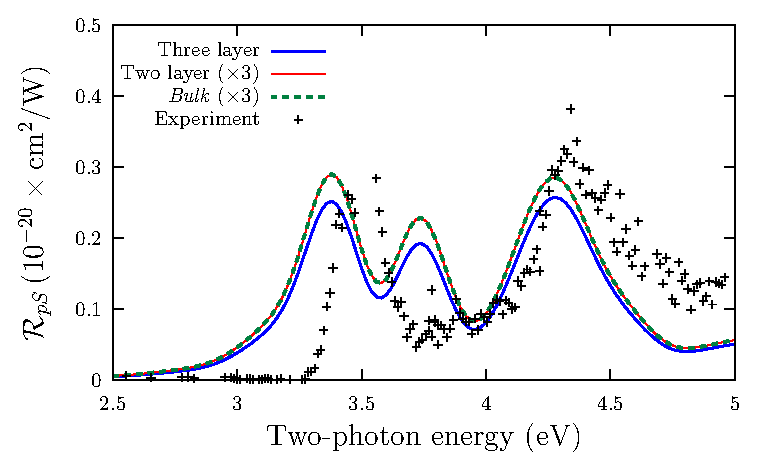
\includegraphics[width=0.48\textwidth]{figures/03-results/shgyield/fig3}
\caption{(Color online) Comparison between theoretical models (see Table
\ref{tab:models}) and experiment for $\mathcal{R}_{pS}$, for
$\theta=65^{\circ}$. We use a scissors value of $\hbar\Delta = 0.7\,\text{eV}$.
The $\chi^{\mathrm{abc}}(-2\omega;\omega,\omega)$ components are broadened with
$\sigma=0.05\,\text{eV}$, and then $\mathcal{R}_{pS}$ is broadened with
$\sigma=0.10\,\text{eV}$. Experimental data taken from Ref.
\cite{mejiaPRB02}.\label{fig:RpS}}
\end{figure}

The main issue to address here is the discrepancy between the intensity of the
E$_{1}$ peak. In the theoretical curves, the peaks differ only slightly in
overall intensity. Conversely, the experimental E$_{1}$ peak is significantly
smaller than the E$_{2}$ peak. This may be due to the effects of oxidation on
the surface. Ref. \cite{bergfeldPRL04} features similar data to those of
Ref. \cite{mejiaPRB02} but focuses on the effects of surface oxidation. We
can see that as time passes during the experiment, the surface becomes more
oxidized, and the E$_{1}$ peak diminishes substantially, as shown by the
experimental data taken 5 hours after initial H-termination. This may be enough
time to slightly reduce the E$_{1}$ peak intensity, as can be observed here.

In Fig. \ref{fig:mitchellRpS}, we compare the theoretical $\mathcal{R}_{pS}$
with experimental data from Ref. \cite{mitchellSS01}; this data, however,
only encompasses the E$_{1}$ peaks, and was obtained at room temperature. We
consider an angle of incidence $\theta=45^\circ$ and an azimuthal angle
$\phi=30^\circ$ to match these experimental conditions. As in the previous
comparison, the E$_{1}$ peak is slightly redshifted compared to experiment. The
intensity of the theoretical yield is smaller than the experimental yield for
all three models. The measurements presented in Ref. \cite{mitchellSS01}
were taken very shortly after the surface had been prepared, and the surface
itself was prepared with a high degree of quality and measured at room
temperature. Peak position compared to theory is slightly improved under these
conditions. As before, the three layer model is closer in intensity to the
experimental spectrum.

\begin{figure}[b]
\centering
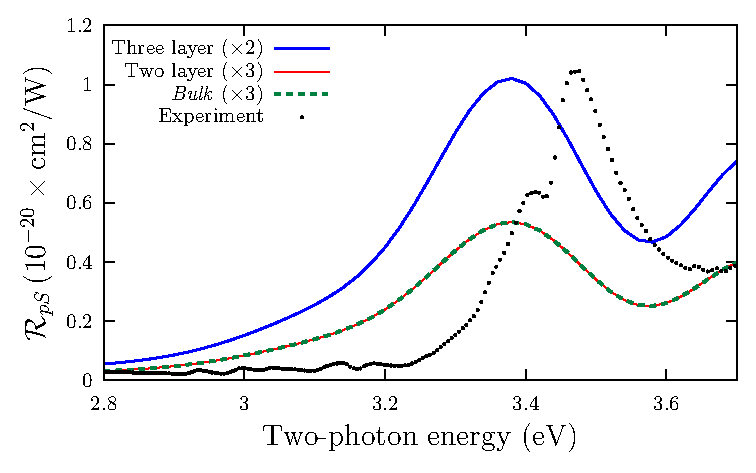
\includegraphics[width=0.48\textwidth]{figures/03-results/shgyield/fig4}
\caption{(Color online) Comparison between theoretical models (see Table
\ref{tab:models}) and experiment for $\mathcal{R}_{pS}$, for $\theta=45^\circ$.
We use a scissors value of $\hbar\Delta = 0.7\,\text{eV}$. The
$\chi^{\mathrm{abc}}(-2\omega;\omega,\omega)$ components are broadened with
$\sigma=0.05\,\text{eV}$, and then $\mathcal{R}_{pS}$ is broadened with
$\sigma=0.10\,\text{eV}$. Experimental data taken from Ref.
\cite{mitchellSS01}.\label{fig:mitchellRpS}}
\end{figure}

In both comparisons, the E$_{1}$ peak position is slightly redshifted. It is well
known that temperature causes shifting in the peak position of SHG
spectra.\cite{dadapPRB96} We showed in the previous section that our calculation
is closer to low temperature measurements. It is likely that low temperature
measurements for the SHG yield will lead to more closely matched results.

Both the two layer and bulk models are identical and roughly 3 times smaller
than the experiment. We can see from Eq. \eqref{eq:rpS} that $\mathcal{R}_{pS}$
only has $1\omega$ terms ($\varepsilon_{\ell}(\omega)$ and $k_{b}$). For both of
these models, the fundamental fields are evaluated in the bulk, which means that
the only change to Eq. \eqref{eq:rpS} is that $\varepsilon_{\ell}(\omega)
\rightarrow \varepsilon_{b}(\omega)$. Additionally, $\Gamma^{\ell}_{pS}$ also
remains identical between the two models and has no $2\omega$ terms in the
denominator. Therefore, $r_{pS}$ is identical between these two models.
Ultimately, the three layer model best reproduces both the lineshape and the
intensity of the experimental spectrum.

Per Eq. \eqref{eq:rpS}, the intensity of $\mathcal{R}_{pS}$ depends only on
$\chi_{\parallel\parallel\parallel}$, which is not affected by local field
effects.\cite{tancognedejean:tel-01235611} These effects are neglected in this
calculation, but $\mathcal{R}_{pS}$ maintains an accurate lineshape and provides
a good quantitative description of the experimental SHG yield. We note that both
the calculated and experimental spectra show two-photon resonances at the
energies corresponding to the critical point transitions of bulk Si. We also see
that the SHG yield drops rapidly to zero below E$_{1}$, which is consistent with
the absence of surface states due to the H saturation on the surface. This
observation holds true for all three polarization cases studied here.

Lastly, in Fig. \ref{fig:improvements} we provide an overview of the different
levels of approximation proposed in this article. All curves here were
calculated using the three layer model. The long dashed line depicts the effect
of excluding the contribution from the nonlocal part of the pseduopotentials.
This is consistent with the results reported in Ref. \cite{andersonPRB15},
where the exclusion of this term increases the intensity of the components of
$\boldsymbol{\chi}(-2\omega;\omega,\omega)$ by approximately 15\% to 20\%. We
also notice that the E$_{1}$ peak is larger than the E$_{2}$ peak, contrasting
with the experiment, where the E$_{1}$ peak is smaller than E$_{2}$. Lastly, the
thin solid line depicts the full calculation with a scissors value of
$\hbar\Delta = 0$. We notice that the spectrum is almost rigidly redshifted as
this H-saturated surface has no electronic surface states.\cite{andersonPRB15}
Thus, this demonstrates the importance of including the scissors correction to
accurately reproduce the experimental spectrum. In summary, the inclusion of the
contribution from the nonlocal part of the pseudopotentials and the scissors
operator on top of the three layer model gives a much better comparison with the
experimental data.

\begin{figure}[b]
\centering
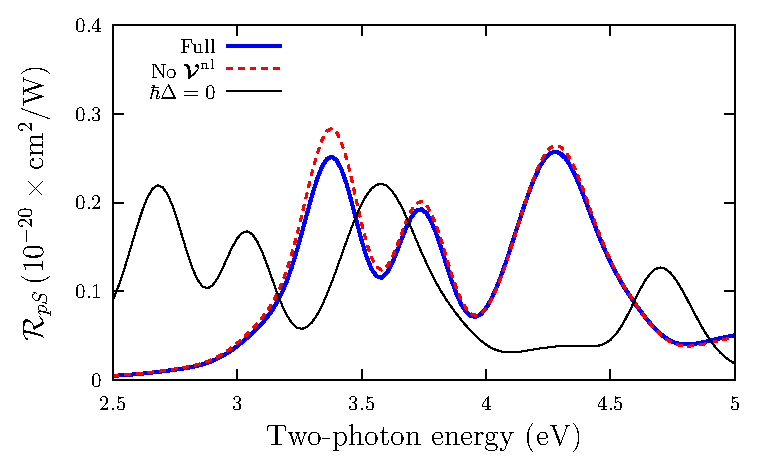
\includegraphics[width=0.48\textwidth]{figures/03-results/shgyield/fig5}
\caption{(Color online) Calculated results for $\mathcal{R}_{pS}$ for the
different levels of approximation proposed in this article. All curves were
calculated using the three layer model. We take $\theta=65^{\circ}$ for this
plot. See text for full details. The
$\chi^{\mathrm{abc}}(-2\omega;\omega,\omega)$ components are broadened with
$\sigma=0.05\,\text{eV}$, and then $\mathcal{R}_{pS}$ is broadened with
$\sigma=0.10\,\text{eV}$.
\label{fig:improvements}}
\end{figure}


\subsection{Calculated \texorpdfstring{$\mathcal{R}_{sP}$}{RsP} compared to
experiment}\label{sec:RsP}

Next, we analyze and compare the calculated $\mathcal{R}_{sP}$ spectra with
experimental data from Ref. \cite{mejiaPRB02}. We again adhere to the
experimental setup by taking an angle of incidence $\theta=65^{\circ}$ and an
azimuthal angle $\phi=30^\circ$. From Fig. \ref{fig:RsP}, we can immediately
appreciate that the overall intensity of $\mathcal{R}_{sP}$ is one order of
magnitude lower than $\mathcal{R}_{pS}$. The experimental data is far noisier
than in the other cases but we can still discern the E$_{1}$ and E$_{2}$ peaks.
As with our previous comparisons, the three layer model accurately matches both
the intensity and the lineshape of the experimental spectrum. It produces a
curve that is very close to the experimental intensity with good proportional
heights for the calculated E$_{1}$ and E$_{2}$ peaks. In contrast, the two layer
model is 100 times more intense than experiment and produces an enlarged E$_{2}$
peak. The bulk model is ten times smaller with a good lineshape.

The differences between the two layer and bulk models are not derived from Eq.
\eqref{eq:rsP}, as the $\varepsilon_{b}(2\omega)$ does not change and the second
term vanishes for this azimuthal angle of $\phi = 30$. However,
$\Gamma^{\ell}_{sP}$ does cause a significant change in the intensity as there
is an $\varepsilon_{\ell}(2\omega)$ term in the denominator. This will become
$\varepsilon_{v}(2\omega) = 1$ for the two layer model, and
$\varepsilon_{b}(2\omega)$ in the bulk model. This accounts for the significant
difference between the intensity of the two models, while the lineshape remains
mostly consistent.

At higher energies, the theoretical curve is blueshifted as compared to the
experiment. We consider that the likely explanation for this is the inclusion of
the scissor operator, which does not adequately correct the transitions
occurring at these higher energies. A full GW calculation would be well suited
for this task, but is beyond the scope of this paper.

\begin{figure}[t]
\centering
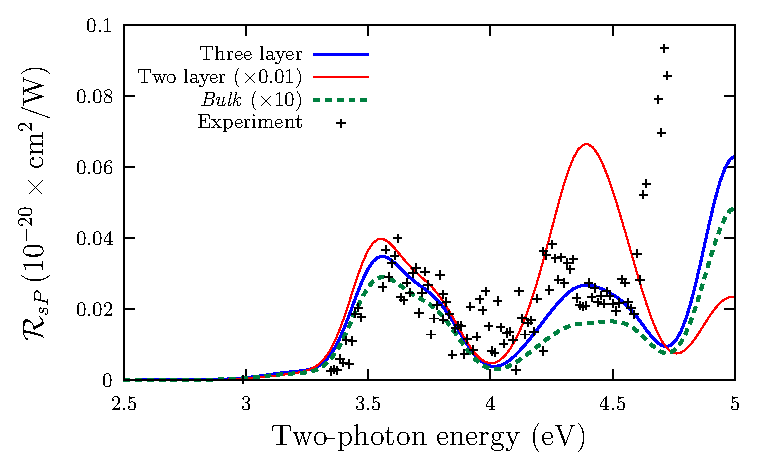
\includegraphics[width=0.48\textwidth]{figures/03-results/shgyield/fig6}
\caption{(Color online) Comparison between theoretical models (see Table
\ref{tab:models}) and experiment for $\mathcal{R}_{sP}$, for
$\theta=65^{\circ}$. We use a scissors value of $\hbar\Delta = 0.7\,\text{eV}$.
The $\chi^{\mathrm{abc}}(-2\omega;\omega,\omega)$ components are broadened with
$\sigma=0.05\,\text{eV}$, and then $\mathcal{R}_{sP}$ is broadened with
$\sigma=0.10\,\text{eV}$. Experimental data taken from Ref.
\cite{mejiaPRB02}.\label{fig:RsP}}
\end{figure}


\subsection{Calculated \texorpdfstring{$\mathcal{R}_{pP}$}{RpP} compared to
experiment}\label{sec:RpP}

We present $\mathcal{R}_{pP}$ compared to experimental data from Ref.
\cite{mejiaPRB02} in Fig. \ref{fig:RpP}. We note that peak position for
the three layer model is similar to experiment with the overall intensity being
only two times larger. The E$_{2}$ peak is blueshifted by around 0.3\,eV, and
the yield does not go to zero after 4.75\,eV. The two layer model has good
lineshape, but it is 40 times more intense than experiment. The calculated
E$_{2}$ peak is similar, but the E$_{1}$ peak lacks the sharpness present in the
experiment. The bulk model is very close to the lineshape of the three layer
model, but with four times less intensity. From Eq. \eqref{eq:rpP}, we see that
$\mathcal{R}_{pP}$ has several $2\omega$ terms that will change between models.
This will have a deep effect on the lineshape. Coupled to $\Gamma^{\ell}_{pP}$,
which also has $\varepsilon_{\ell}(2\omega)$ in the denominator, and we have a
significant difference in both lineshape and intensity between the two layer and
bulk models.

Reviewing Eq. \eqref{eq:rpP}, we see that $\mathcal{R}_{pP}$ is by far the most
involved calculation, since it includes all four nonzero components. In
particular, $\chi_{\perp\perp\perp}$ and $\chi_{\parallel\parallel\perp}$
include out-of-plane incoming fields. These are affected by local field effects
that can change both intensity and peak
position.\cite{tancognedejean:tel-01235611} Including these effects is
computationally very expensive and is beyond the scope of this paper. We
speculate that $\mathcal{R}_{pP}$ requires the proper inclusion of these effects
in order to accurately describe the experimental peaks.

\begin{figure}[b]
\centering
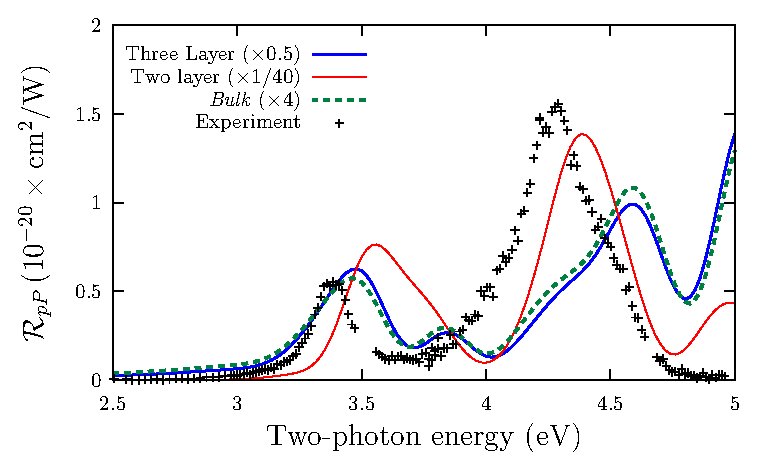
\includegraphics[width=0.48\textwidth]{figures/03-results/shgyield/fig7}
\caption{(Color online) Comparison between theoretical models (see Table
\ref{tab:models}) and experiment for $\mathcal{R}_{pP}$, for
$\theta=65^{\circ}$. We use a scissors value of $\hbar\Delta = 0.7\,\text{eV}$.
The $\chi^{\mathrm{abc}}(-2\omega;\omega,\omega)$ components are broadened with
$\sigma=0.05\,\text{eV}$, and then $\mathcal{R}_{pP}$ is broadened with
$\sigma=0.10\,\text{eV}$. Experimental data taken from Ref.
\cite{mejiaPRB02}.\label{fig:RpP}}
\end{figure}

Lastly, in Fig. \ref{fig:mitchellRpP} we compare to Ref.
\cite{mitchellSS01}. The three layer model is, as before, very close in
both peak position and intensity. Intensity is improved with the calculated
spectrum at almost the same intensity as the experiment. This provides a more
compelling argument against the two layer model than Fig. \ref{fig:RpP}. The two
layer model is 20 times more intense and blueshifted by around 0.1\,eV. As
mentioned before, this surface is of very high quality with measurements taken
shortly after surface preparation. As before, the bulk model is intermediate in
both intensity and lineshape. Under these conditions, the three layer model very
accurately reproduces the E$_{1}$ peak over the two layer and bulk models.

\begin{figure}[t]
\centering
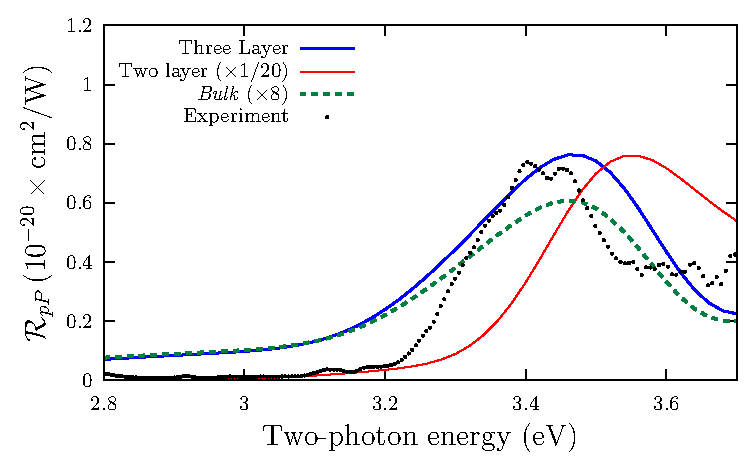
\includegraphics[width=0.48\textwidth]{figures/03-results/shgyield/fig8}
\caption{(Color online) Comparison between theoretical models (see Table
\ref{tab:models}) and experiment for $\mathcal{R}_{pP}$, for
$\theta=45^{\circ}$. We use a scissors value of $\hbar\Delta = 0.7\,\text{eV}$.
The $\chi^{\mathrm{abc}}(-2\omega;\omega,\omega)$ components are broadened with
$\sigma=0.05\,\text{eV}$, and then $\mathcal{R}_{pP}$ is broadened with
$\sigma=0.10\,\text{eV}$. Experimental data taken from Ref.
\cite{mitchellSS01}.\label{fig:mitchellRpP}}
\end{figure}


\include{chapters/04-conclusion}

\part{Appendices}
\appendix
\documentclass[aps,letterpaper]{revtex4}
\usepackage{amsmath}
\usepackage[colorlinks=true]{hyperref}

\input{../../base/bms}

\begin{document}

\section{\texorpdfstring{$\mathbf{r}_{e}$ and $\mathbf{r}_{i}$}{re and ri}}
\label{app:re_ri}

In this appendix, we derive the expressions for the matrix elements of the
electron position operator $\mathbf{r}$. The $r$ representation of the Bloch
states is given by
\begin{equation}\label{bloch}
\psi_{n\mathbf{k}}(\mathbf{r})=\langle\mathbf{r}\vert n\mathbf{k}\rangle =
\sqrt{\frac{\Omega}{8\pi^{3}}}
e^{i\mathbf{k} \cdot \mathbf{r}}u_{n\mathbf{k}}(\mathbf{r}),
\end{equation}
where $u_{n\mathbf{k}}(\mathbf{r}) = u_{n\mathbf{k}}(\mathbf{r} + \mathbf{R})$
is cell periodic, and
\begin{equation}\label{normal}
\int_{\Omega}
u_{n\mathbf{k}}^{*}(\mathbf{r})u_{m\mathbf{k}'}(\mathbf{r})\,d^{3}r
= \delta_{nm}\delta_{\mathbf{\mathbf{k},\mathbf{k}'}},
\end{equation}
and $\Omega$ is the unit cell volume.

The key ingredient in the calculation are the matrix elements of the position
operator $\mathbf{r}$. We start from the basic relation
\begin{equation}\label{nbraket}
\langle n\mathbf{k}\vert m\mathbf{k}'\rangle =
\delta_{nm}\delta(\mathbf{k} - \mathbf{k}'),
\end{equation}
and take its derivative with respect to $\mathbf{k}$ as follows. On one hand,
\begin{equation}\label{ddk1}
\frac{\partial}{\partial\mathbf{k}}
\langle n\mathbf{k}\vert m\mathbf{k}'\rangle =
\delta_{nm}\frac{\partial}{\partial\mathbf{k}}\delta(\mathbf{k} - \mathbf{k}'),
\end{equation}
and on the other,
\begin{equation}\label{dkbraket}
\frac{\partial}{\partial\mathbf{k}}\braket{n\mathbf{k}}{m\mathbf{k}'}
= \frac{\partial}{\partial\mathbf{k}}\int
\langle n\mathbf{k}\vert \mathbf{r}\rangle
\langle \mathbf{r}\vert m\mathbf{k}'\rangle
\,d\mathbf{r} 
= \int
\left(
\frac{\partial}{\partial\mathbf{k}}
\psi^{*}_{n\mathbf{k}}(\mathbf{r})
\right)
\psi_{m\mathbf{k}'}(\mathbf{r})\,d\mathbf{r}.
\end{equation}
The derivative of the wavefunction is simply given by
\begin{equation}\label{dpsi}
\frac{\partial}{\partial\mathbf{k}}\psi^{*}_{n\mathbf{k}}(\mathbf{r})
= \sqrt{\frac{\Omega}{8\pi^{3}}}
\left(
\frac{\partial}{\partial\mathbf{k}}
u^{*}_{n\mathbf{k}}(\mathbf{r})
\right)
e^{-i\mathbf{k}\cdot\mathbf{r}} - i\mathbf{r}\psi^{*}_{n\mathbf{k}}(\mathbf{r}).
\end{equation}
Substituting into Eq. \eqref{dkbraket}, we obtain
\begin{align}\label{dkbraket2}
\frac{\partial}{\partial\mathbf{k}}\braket{n\mathbf{k}}{m\mathbf{k}'}
&= \sqrt{\frac{\Omega}{8\pi^{3}}}\int
\left(
\frac{\partial}{\partial\mathbf{k}}
u^{*}_{n\mathbf{k}}(\mathbf{r})\right)e^{-i\mathbf{k}\cdot\mathbf{r}}
\psi_{m\mathbf{k}'}(\mathbf{r})\,d\mathbf{r} 
- i\int\psi^{*}_{n\mathbf{k}}(\mathbf{r})\mathbf{r}
  \psi_{m\mathbf{k}'}(\mathbf{r})\,d\mathbf{r}\nonumber \\
&= \frac{\Omega}{8\pi^{3}}\int
  e^{-i(\mathbf{k}-\mathbf{k}')\cdot\mathbf{r}}
  \left(
  \frac{\partial}{\partial\mathbf{k}}u^{*}_{n\mathbf{k}}(\mathbf{r})
  \right)
u_{m\mathbf{k}'}(\mathbf{r})\,d\mathbf{r}
- i \bra{n\mathbf{k}}\hat{\mathbf{r}}\ket{m\mathbf{k}'}.
\end{align}
Restricting $\mathbf{k}$ and $\mathbf{k}'$ to the first Brillouin zone, we use
the following result that is valid for any periodic function
$f(\mathbf{r}) = f(\mathbf{r} + \mathbf{R})$,
\begin{align}\label{periodic}
\int e^{i(\mathbf{q}-\mathbf{k})\cdot\mathbf{r}}f(\mathbf{r})\,d^{3}r =
\frac{8\pi^{3}}{\Omega}\delta(\mathbf{q} - \mathbf{k})
\int_{\Omega}f(\mathbf{r})\,d^{3}r,
\end{align}
to finally write \cite{blountSSP62}
\begin{align}\label{dkbraket3}
\frac{\partial}{\partial\mathbf{k}}
\langle n\mathbf{k}\vert m\mathbf{k}'\rangle
&= \delta(\mathbf{k}-\mathbf{k}')\int_{\Omega}
\left(
\frac{\partial}{\partial\mathbf{k}} u^{*}_{n\mathbf{k}}(\mathbf{r})
\right)
u_{m\mathbf{k}}(\mathbf{r})\,d\mathbf{r}
-i\bra{n\mathbf{k}}\hat{\mathbf{r}}\ket{m\mathbf{k}'}.
\end{align}
From
\begin{align}\label{dnm1}
\int_{\Omega}u_{m\mathbf{k}} u^{*}_{n\mathbf{k}}\,d\mathbf{r} = \delta_{nm},
\end{align}
we easily find that
\begin{align}\label{dnm2}
\int_{\Omega}
\left(
\frac{\partial}{\partial\mathbf{k}} u_{m\mathbf{k}}(\mathbf{r})
\right)
u^{*}_{n\mathbf{k}}(\mathbf{r})\,d\mathbf{r}
= -\int_{\Omega}u_{m\mathbf{k}}(\mathbf{r})
\left(
\frac{\partial}{\partial\mathbf{k}} u^{*}_{n\mathbf{k}}(\mathbf{r})
\right)\,d\mathbf{r}.
\end{align}
Therefore, we define
\begin{align}\label{zeta}
\boldsymbol{\xi}_{nm}(\mathbf{k}) \equiv
i\int_{\Omega}u^{*}_{n\mathbf{k}}(\mathbf{r})\nabla_{\mathbf{k}}
u_{m\mathbf{k}}(\mathbf{r})\,d\mathbf{r},
\end{align} 
with $\nabla_{\mathbf{k}} = \partial/\partial\mathbf{k}$. Now, from Eqs.
\eqref{ddk1}, \eqref{dkbraket2}, and  \eqref{zeta}, we have that the matrix
elements of the position operator of the electron are given by
\begin{align}\label{erre}
\langle n\mathbf{k}\vert \hat{\mathbf{r}} \vert m\mathbf{k}'\rangle 
= \delta(\mathbf{k}-\mathbf{k}')\boldsymbol{\xi}_{nm}(\mathbf{k})
+ i\delta_{nm}\nabla_{\mathbf{k}}\delta(\mathbf{k}-\mathbf{k}'),
\end{align}
Then, from Eq. \eqref{erre} and writing $\hat{\mathbf{r}} = \hat{\mathbf{r}}_{e}
+ \hat{\mathbf{r}}_{i}$, with $\hat{\mathbf{r}}_{e}$ ($\hat{\mathbf{r}}_{i}$)
the interband (intraband) part, we obtain that
\begin{align}\label{rnmi}
\langle n\mathbf{k}\vert \hat{\mathbf{r}}_{i} \rangle m\mathbf{k}'\vert
&= \delta_{nm}
\left[
  \delta(\mathbf{k}-\mathbf{k}')\boldsymbol{\xi}_{nn}(\mathbf{k})
+ i\nabla_{\mathbf{k}}\delta(\mathbf{k} - \mathbf{k}')
\right],\\
\langle n\mathbf{k}\vert \hat{\mathbf{r}}_e \rangle m\mathbf{k}'\vert
&= (1 - \delta_{nm})\delta(\mathbf{k}-\mathbf{k}')
   \boldsymbol{\xi}_{nm}(\mathbf{k}).
\label{rnme}
\end{align} 

To proceed, we relate Eq. \eqref{rnme} to the matrix elements of the momentum
operator as follows. For the intraband part, we derive the following general
result,
\begin{align}\label{conmri}
\bra{n\mathbf{k}}[\hat{\mathbf{r}}_{i},\hat\calo]\ket{m\mathbf{k}'}
&=
\sum_{\ell,\mathbf{k}''}
\left(
\bra{n\mathbf{k}}
\hat{\mathbf{r}}_{i}
\ket{\ell\mathbf{k}''}
\bra{\ell\mathbf{k}''}
\hat\calo
\ket{m\mathbf{k}'}
\right.
\nonumber \\
&
\left.
-
\bra{n\mathbf{k}}
\hat\calo
\ket{\ell\mathbf{k}''}
\bra{\ell\mathbf{k}''}
\hat{\mathbf{r}}_{i}
\ket{m\mathbf{k}'}
\right)
\nonumber \\
&=
\sum_{\ell}
\left(
\bra{n\mathbf{k}}
\hat{\mathbf{r}}_{i}
\ket{\ell\mathbf{k}'}
\calo_{\ell m}(\mathbf{k}')
\right.
\nonumber \\
&
\left.
-
\calo_{n\ell}(\mathbf{k})
\ket{\ell\mathbf{k}}
\bra{\ell\mathbf{k}}
\hat{\mathbf{r}}_{i}
\ket{m\mathbf{k}'}
\right)
,
\end{align}
where we have taken
$\bra{n\mathbf{k}}\hat\calo\ket{\ell\mathbf{k}''}=\delta(\mathbf{k}-\mathbf{k}'')\calo_{n\ell}(\mathbf{k})$.
We substitute Eq. \eqref{rnmi}, to obtain
\begin{align}\label{conmri2}
\sum_{\ell}&
\left(
\delta_{n\ell}\left[\delta(\mathbf{k}-\mathbf{k}')\boldsymbol{\xi}_{nn}(\mathbf{k})
+i\nabla_{\mathbf{k}}\delta(\mathbf{k}-\mathbf{k}')\right]
\calo_{\ell m}(\mathbf{k}')
\right.
\nonumber \\
&
\left.
-
\calo_{n\ell}(\mathbf{k})
\delta_{\ell m}\left[\delta(\mathbf{k}-\mathbf{k}')\boldsymbol{\xi}_{mm}(\mathbf{k})
+i\nabla_{\mathbf{k}}\delta(\mathbf{k}-\mathbf{k}')\right]
\right)
\nonumber\\
&=
\left(
\left[\delta(\mathbf{k}-\mathbf{k}')\boldsymbol{\xi}_{nn}(\mathbf{k})
+i\nabla_{\mathbf{k}}\delta(\mathbf{k}-\mathbf{k}')\right]
\calo_{n m}(\mathbf{k}')
\right.
\nonumber \\
&-
\left.
\calo_{nm}(\mathbf{k})
\left[\delta(\mathbf{k}-\mathbf{k}')\boldsymbol{\xi}_{mm}(\mathbf{k})
+i\nabla_{\mathbf{k}}\delta(\mathbf{k}-\mathbf{k}')\right]
\right)
\nonumber\\
&=
\delta(\mathbf{k}-\mathbf{k}')
\calo_{nm}(\mathbf{k})
\left(
\boldsymbol{\xi}_{nn}(\mathbf{k})
-
\boldsymbol{\xi}_{mm}(\mathbf{k})
\right)
+i\calo_{n m}(\mathbf{k}')
\nabla_{\mathbf{k}}
\delta(\mathbf{k}-\mathbf{k}')
\nonumber \\
&+i
\delta(\mathbf{k}-\mathbf{k}')
\nabla_{\mathbf{k}}
\calo_{n m}(\mathbf{k})
-
i\calo_{n m}(\mathbf{k}')
\nabla_{\mathbf{k}}\delta(\mathbf{k}-\mathbf{k}')
\nonumber \\
&=
i\delta(\mathbf{k}-\mathbf{k}')
\bigg(
\nabla_{\mathbf{k}}
\calo_{n m}(\mathbf{k})
-
i
\calo_{nm}(\mathbf{k})
\left(
\boldsymbol{\xi}_{nn}(\mathbf{k})
-
\boldsymbol{\xi}_{mm}(\mathbf{k})
\right)
\bigg)
\nonumber \\
&\equiv
i\delta(\mathbf{k}-\mathbf{k}')(\calo_{nm})_{;\mathbf{k}}
.
\end{align}
Then,
\begin{align}\label{conmri3}
\bra{n\mathbf{k}}[\hat{\mathbf{r}}_{i},\hat\calo]\ket{m\mathbf{k}'}
=i\delta(\mathbf{k}-\mathbf{k}')(\calo_{nm})_{;\mathbf{k}}
,
\end{align}   
with
\begin{align}\label{gendev}
(\calo_{nm})_{;\mathbf{k}}=
\nabla_{\mathbf{k}}
\calo_{n m}(\mathbf{k})
-  
i
\calo_{nm}(\mathbf{k})
\left(
\boldsymbol{\xi}_{nn}(\mathbf{k})
-
\boldsymbol{\xi}_{mm}(\mathbf{k})
\right)
,
\end{align}  
the generalized derivative of $\calo_{nm}$ with respect to $\mathbf{k}$.
Note that the highly singular term $\nabla_{\mathbf{k}}\delta(\mathbf{k}-\mathbf{k}')$
cancels in Eq. \eqref{conmri2}, thus giving a well defined commutator
of the intraband position operator with an arbitrary operator $\hat\calo$.
We use Eq. \eqref{chon.98} and \eqref{conmri3}  in the next section.

\bibliographystyle{unsrt}
\bibliography{/Users/sma/Dropbox/docs/academics/master}

\end{document}
%reri A
\include{appendices/appendix02-vnl}%appvnl B
\chapter{\texorpdfstring{$V^{\gs,\rma,\ell}_{nm}$}{Vnm} and \texorpdfstring{$\Big({\cal V}^{\gs,\rma,\ell}_{nm}\Big)_{;k^\rmb}$}{(Vnm);kb} }\label{calvs}

From Eq.~\eqref{vopii}
\begin{align}\label{a.1}
\left(
\calv^{\gs,\rma,\ell}_{nm}
\right)_{;k^\rmb}
=
\left(
\calv^{\lda,\rma,\ell}_{nm}
\right)_{;k^\rmb}
+
\left(
\calv^{\cals,\rma,\ell}_{nm}
\right)_{;k^\rmb}
.
\end{align} 
For the LDA term we have
\begin{align}\label{a.2}
\calv^{\lda,\rma,\ell}_{nm}
&=
\frac{1}{2}\left(  
v^{\lda,\rma}\calc^\ell+\calc^\ell v^{\lda,\rma}
\right)_{nm}
\nonumber\\
&=
\frac{1}{2}\sum_q\left(  
v^{\lda,\rma}_{nq}\calc^\ell_{qm}+\calc^\ell_{nq} v^{\lda,\rma}_{qm}
\right)
\nonumber\\
\left(\calv^{\lda,\rma}_{nm}\right)_{;k^\rmb}
&=
\frac{1}{2}\sum_q\left(  
v^{\lda,\rma}_{nq}\calc^\ell_{qm}+\calc^\ell_{nq} v^{\lda,\rma}_{qm}
\right) _{;k^\rmb}
\nonumber\\
&=
\frac{1}{2}\sum_q\left(
(v^{\lda,\rma}_{nq})_{;k^\rmb}\calc^\ell_{qm}
+   
v^{\lda,\rma}_{nq}(\calc^\ell_{qm})_{;k^\rmb}
+
(\calc^\ell_{nq})_{;k^\rmb} v^{\lda,\rma}_{qm}
+
\calc^\ell_{nq} (v^{\lda,\rma}_{qm})_{;k^\rmb}
\right)
,
\end{align}   
where we omitted $\bfk$ in all quantities.
From Eq.~\eqref{vnln.2} we know that $\bfv^\nl_{nm}(\bfk)$
 can be readily
calculated,
and from Appendix \ref{calpcalc}, both $v^a_{nm}$ and
$\calc_{nm}^\ell$ are also known quantities, 
 and thus the
$\bfv^\lda_{nm}(\bfk)$ are known, which in turns means that 
$\calv^{\lda,\rma,\ell}_{nm}$ are also known.
For the generalized derivative 
$(\bfv^\lda_{nm}(\bfk))_{;\bfk}$ we use Eq.~\eqref{chon.98}
to write
\begin{align}\label{a.3}
(v^{\lda,\rma}_{nm})_{;k^\rmb}
&=  
im_e(\go^\lda_{nm}r^\rma_{nm})_{;k^\rmb}
\nonumber\\
&=  
im_e(\go^\lda_{nm})_{;k^\rmb} r^\rma_{nm}
+  
im_e\go^\lda_{nm}(r^\rma_{nm})_{;k^\rmb}
\nonumber\\
&=  
im_e\gD^b_{nm}r^\rma_{nm}
+ 
im_e\go^\lda_{nm}(r^\rma_{nm})_{;k^\rmb}
\quad\mathrm{for}\quad n\ne m
,
\end{align} 
where we used Eq \eqref{eli.13} and $(r^\rma_{nm})_{;k^\rmb}$ is given
in Eq.~\eqref{na_rgendevn}.

Likewise,
\begin{align}\label{a.3b}
\calv^{\cals,\rma,\ell}_{nm}
&=
\frac{1}{2}\left(  
v^{\cals,\rma}\calc^\ell+\calc^\ell v^{\cals,\rma}
\right)_{nm}
\nonumber\\
&=
\frac{1}{2}\sum_q\left(  
v^{\cals,\rma}_{nq}\calc^\ell_{qm}+\calc^\ell_{nq} v^{\cals,\rma}_{qm}
\right)
\nonumber\\
\left(\calv^{\cals,\rma}_{nm}\right)_{;k^\rmb}
&=
\frac{1}{2}\sum_q\left(  
v^{\cals,\rma}_{nq}\calc^\ell_{qm}+\calc^\ell_{nq} v^{\cals,\rma}_{qm}
\right) _{;k^\rmb}
\nonumber\\
&=
\frac{1}{2}\sum_q\left(
(v^{\cals,\rma}_{nq})_{;k^\rmb}\calc^\ell_{qm}
+   
v^{\cals,\rma}_{nq}(\calc^\ell_{qm})_{;k^\rmb}
+
(\calc^\ell_{nq})_{;k^\rmb} v^{\cals,\rma}_{qm}
+
\calc^\ell_{nq} (v^{\cals,\rma}_{qm})_{;k^\rmb}
\right)
,
\end{align}   
where $v^{\cals,\rma}_{nm}(\bfk)$ are given in Eq.~\eqref{chon.2}
and
$(v^{\cals,\rma}_{nm})_{;k^\rmb}$ is given in Eq. A(6) of
Ref.~\cite{cabellosPRB09},
\begin{align}\label{choni.1}
(v^{\cals,\rma}_{nm})_{;k^\rmb}=i\gD f_{mn}
(r^\rma_{nm})_{;k^\rmb}
.
\end{align}

To evaluate $(\calc^\ell_{nm})_{;k^\rma}$, we use the fact that as
$\calc^\ell(z)$ is only a function of the $z$ coordinate, its commutator
with $\bfr$ is zero, then,
\begin{align}\label{a.4}
\bra{n\bfk}
\left[r^\rma,\calc^\ell(z)\right]
\ket{m\bfk'}
&=
\bra{n\bfk}
\left[r_e^\rma,\calc^\ell(z)\right]
\ket{m\bfk'}
+
\bra{n\bfk}
\left[r_i^\rma,\calc^\ell(z)\right]
\ket{m\bfk'}
=
 0
.
\end{align} 
The interband part reduces to,
\begin{align}\label{a.5}
\left[r_e^\rma,\calc^\ell(z)\right]_{nm}
&=
\sum_{q\bfk''}
\left(
\bra{n\bfk}
r_e^\rma
\ket{q\bfk''}
\bra{q\bfk''}
\calc^\ell(z)
\ket{m\bfk'}
-
\bra{n\bfk}
\calc^\ell(z)
 \ket{q\bfk''}
\bra{q\bfk''}
r_e^\rma
\ket{m\bfk'}
\right)
\nonumber\\
&=
\sum_{q\bfk''}
\gd(\bfk-\bfk'')
\gd(\bfk'-\bfk'')
\left(
(1-\gd_{qn})
\xi_{nq}^\rma
\calc^\ell_{qm}
-
(1-\gd_{qm})
\calc^\ell_{nq}
\xi_{qm}^\rma
\right)
\nonumber\\
&=
\gd(\bfk-\bfk')
\left(
\sum_{q}
\left(
\xi_{nq}^\rma
\calc^\ell_{qm}
-
\calc^\ell_{nq}
\xi_{qm}^\rma
\right)
+
\calc^\ell_{nm}(\xi_{mm}^\rma-\xi_{nn}^\rma)
\right)
,
\end{align}
where we used Eq.~\eqref{rnme}, and the $\bfk$ and $z$ dependence is implicitly
understood. From Eq.~\eqref{conmri3} the intraband part is,
\begin{align}\label{a.6}
\bra{n\bfk}[\hat\bfr_i,\calc^\ell(z)]\ket{m\bfk'}
=i\gd(\bfk-\bfk')(\calc^\ell_{nm})_{;\bfk}
,
\end{align}
then from Eq.~\eqref{a.4}
\begin{align}\label{a.7}
&
\left(
(\calc^\ell_{nm})_{;\bfk}
-i
\sum_{q}
\left(
\xi_{nq}^\rma
\calc^\ell_{qm}
-
\calc^\ell_{nq}
\xi_{qm}^\rma
\right)
-i
\calc^\ell_{nm}(\xi_{mm}^\rma-\xi_{nn}^\rma)
\right) i\gd(\bfk-\bfk')
=0
\nonumber\\
\frac{1}{i}(\calc^\ell_{nm})_{;\bfk}
&=
\sum_{q}
\left(
\xi_{nq}^\rma
\calc^\ell_{qm}
-
\calc^\ell_{nq}
\xi_{qm}^\rma
\right)
+
\calc^\ell_{nm}(\xi_{mm}^\rma-\xi_{nn}^\rma)
\nonumber\\
&=
\sum_{q\ne nm}
\left(
\xi_{nq}^\rma
\calc^\ell_{qm}
-
\calc^\ell_{nq}
\xi_{qm}^\rma
\right)
+
\left(
\xi_{nn}^\rma
\calc^\ell_{nm}
-
\calc^\ell_{nn}
\xi_{nm}^\rma
\right)_{q=n}
+
\left(
\xi_{nm}^\rma
\calc^\ell_{mm}
-
\calc^\ell_{nm}
\xi_{mm}^\rma
\right)_{q=m}
\nonumber\\
&+
\calc^\ell_{nm}(\xi_{mm}^\rma-\xi_{nn}^\rma)
\nonumber\\
(\calc^\ell_{nm})_{;\bfk}
&=
i\sum_{q\ne nm}
\left(
\xi_{nq}^\rma
\calc^\ell_{qm}
-
\calc^\ell_{nq}
\xi_{qm}^\rma
\right)
+i\xi_{nm}^\rma(\calc^\ell_{mm}-\calc^\ell_{nn})
\nonumber\\
&=
i\sum_{q\ne nm}
\left(
r_{nq}^\rma 
\calc^\ell_{qm}
-
\calc^\ell_{nq}
r_{qm}^\rma 
\right) 
+ir_{nm}^\rma(\calc^\ell_{mm}-\calc^\ell_{nn}) 
\nonumber\\
&=
i \left(
\sum_{q\ne n} 
r_{nq}^\rma 
\calc^\ell_{qm}
-
\sum_{q\ne m}
\calc^\ell_{nq}
r_{qm}^\rma 
\right) 
+ir_{nm}^\rma(\calc^\ell_{mm}-\calc^\ell_{nn}) 
,
\end{align} 
since in every $\xi_{nm}^\rma$, $n\ne m$, thus we replace it by $r^\rma_{nm}$. 
The matrix elements $\calc^\ell_{nm}(\bfk)$ are calculated in Appendix~\ref{calpcalc}. 

For the general
case of
\begin{align}\label{a.8}
\bra{n\bfk}
\left[\hat r^\rma,\hat\calg(\bfr,\bfp)\right]
\ket{m\bfk'}
&=
\calu_{nm}(\bfk)
,
\end{align}
above result would lead to a more general expression, 
\begin{align}\label{a.9}
(\calg_{nm}(\bfk))_{;k^\rma}
&=
\calu_{nm}(\bfk)
+
i\sum_{q\ne(nm)}
\left(
r_{nq}^\rma (\bfk)
\calg_{qm}(\bfk)
-
\calg_{nq}(\bfk)
r_{qm}^\rma (\bfk)
\right)
+ir_{nm}^\rma (\bfk) (\calg_{mm}(\bfk)-\calg_{nn}(\bfk))
.
\nonumber\\
\end{align}
%calvs C
\include{appendices/appendix04-gen_der_omega}%gwk D
\include{appendices/appendix05-calv}%appv E
\include{appendices/appendix06-tnm}%calt F
\include{appendices/appendix07-vc}%calpcalc G
\chapter{Generalized derivative \texorpdfstring{$(\bfr_{nm}(\bfk))_{;\bfk}$} {{rnm};k} for non-local potentials}\label{gdernl}

We obtain the generalized derivative $(\bfr_{nm}(\bfk))_{;\bfk}$ for
the case of a non-local potential in the Hamiltonian.
We start from (see Eq.~\eqref{conhr})
\begin{align}\label{na_hrdab}
[r^{\rma},v^{\lda,\rmb}]
&=
[r^{\rma},v^\rmb]
+ 
[r^{\rma},v^{\nl,\rmb}]
=
\frac{i\hbar}{m_e}\gd_{ab}+
[r^{\rma},v^{\nl,\rmb}]
\equiv  
\tau^{\rma\rmb}
,
\end{align}  
where we used the fact that $[r^\rma,p^\rmb]=i\hbar\gd_{ab}$.
Then,
\begin{align}\label{na_hrdab2}
\bra{n\bfk}[r^{\rma},v^{\lda,\rmb}]\ket{m\bfk'}
=
\bra{n\bfk}\tau^{\rma\rmb}\ket{m\bfk'}
=
\tau^{\rma\rmb}_{nm}(\bfk)\gd(\bfk-\bfk')
,
\end{align}
so
\begin{align}\label{na_hrdab3}
\bra{n\bfk}[r^{\rma}_i,v^{\lda,\rmb}]\ket{m\bfk'}
+
\bra{n\bfk}[r^{\rma}_e,v^{\lda,\rmb}]\ket{m\bfk'}
=
\tau^{\rma\rmb}_{nm}(\bfk)\gd(\bfk-\bfk')
,
\end{align}
where the matrix elements of $\tau^{\rma\rmb}_{nm}(\bfk)$ are calculated in  
Appendix \ref{calt}.  
From Eq.~\eqref{conmri3} and ~\eqref{gendev}
\begin{align}\label{na_rip}
\bra{n\bfk}[r^{\rma}_i,v_\lda^{\rmb}]\ket{m\bfk'}
=i\gd(\bfk-\bfk')(v_{nm}^{\lda,\rmb})_{;k^{\rma}}
\end{align}
\begin{align}\label{na_ripn}
(v^{\lda,\rmb}_{nm})_{;k^{\rma}}=
\nabla_{k^{\rma}}
v^{\lda,\rmb}_{n m}(\bfk)
-
i
v^{\lda,\rmb}_{nm}(\bfk)
\left(
\xi^{\rma}_{nn}(\bfk)
-
\xi^{\rma}_{mm}(\bfk)
\right)
,
\end{align}
and
\begin{align}\label{na_rep}
\bra{n\bfk}[r^{\rma}_e,v^{\lda,\rmb}]\ket{m\bfk'}&=
\sum_{\ell\bfk''}
\bigg(
\bra{n\bfk}r^{\rma}_e\ket{\ell\bfk''}\bra{\ell\bfk''}v^{\lda,\rmb}\ket{m\bfk'}
\nonumber \\
&
-
\bra{n\bfk}v^{\lda,\rmb}\ket{\ell\bfk''}\bra{\ell\bfk''}r^{\rma}_e\ket{m\bfk'}
\bigg)
\nonumber \\
&=
\sum_{\ell\bfk''}
\bigg(
(1-\gd_{n\ell})\gd(\bfk-\bfk'')\xi^{\rma}_{n\ell}
\gd(\bfk''-\bfk')v^{\lda,\rmb}_{\ell m}
\nonumber \\
&-
\gd(\bfk-\bfk'')v^{\lda,\rmb}_{n\ell}
(1-\gd_{\ell m})\gd(\bfk''-\bfk')\xi^{\rma}_{\ell m}
\bigg)
\nonumber \\
&=
\gd(\bfk-\bfk')
\sum_{\ell}
\bigg(
(1-\gd_{n\ell})
\xi^{\rma}_{n\ell}
v^{\lda,\rmb}_{\ell m}
\nonumber \\
&-
(1-\gd_{\ell m})
v^{\lda,\rmb}_{n\ell}
\xi^{\rma}_{\ell m}
\bigg)
\nonumber \\
&=
\gd(\bfk-\bfk')
\bigg(
\sum_{\ell}
\bigg(
\xi^{\rma}_{n\ell}
v^{\lda,\rmb}_{\ell m}
-
v^{\lda,\rmb}_{n\ell}
\xi^{\rma}_{\ell m}
\bigg)
\nonumber \\
&+
v^{\lda,\rmb}_{nm}(\xi^{\rma}_{mm}
-
\xi^{\rma}_{nn}
)
\bigg)
.
\end{align}
Using Eqs.~\eqref{na_rip} and ~\eqref{na_rep}
into Eq.~\eqref{na_hrdab3} gives
\begin{align}\label{na_rapb}
i\gd(\bfk-\bfk')
\bigg(
(v^{\lda,\rmb}_{nm})_{;k^{\rma}}
&
-i
\sum_{\ell}
\bigg(
\xi^{\rma}_{n\ell}
v^{\lda,\rmb}_{\ell m}
-
v^{\lda,\rmb}_{n\ell}
\xi^{\rma}_{\ell m}
\bigg)
\nonumber \\
&
-i
v^{\lda,\rmb}_{nm}(\xi^{\rma}_{mm}
-
\xi^{\rma}_{nn}
)
\bigg)
=
\tau^{\rma\rmb}_{nm}(\bfk)\gd(\bfk-\bfk')
,
\end{align}
then
\begin{align}\label{na_rapb2}
(v^{\lda,\rmb}_{nm})_{;k^{\rma}}&=
-i
\tau^{\rma\rmb}_{nm}
+i
\sum_{\ell}
\bigg(
\xi^{\rma}_{n\ell}
v^{\lda,\rmb}_{\ell m}
-
v^{\lda,\rmb}_{n\ell}
\xi^{\rma}_{\ell m}
\bigg)
+i
v^{\lda,\rmb}_{nm}(\xi^{\rma}_{mm}
-
\xi^{\rma}_{nn}
)
,
\end{align}
and from Eq.~\eqref{na_ripn},
\begin{align}\label{ncogno}
\nabla_{k^{\rma}}v^{\lda,\rmb}_{nm}=
-i\tau^{\rma\rmb}_{nm}
+i
\sum_{\ell}
\bigg(
\xi^{\rma}_{n\ell}
v^{\lda,\rmb}_{\ell m}
-
v^{\lda,\rmb}_{n\ell}
\xi^{\rma}_{\ell m}
\bigg)
.
\end{align}
Now, there are two cases. We use Eq.~\eqref{chon.98}.

\noindent {\it Case} $n=m$
\begin{align}\label{ntita}
\nabla_{k^{\rma}}v^{\lda,\rmb}_{nn}&=
-i\tau^{\rma\rmb}_{nn}
+i
\sum_{\ell}
\bigg(
\xi^{\rma}_{n\ell}
v^{\lda,\rmb}_{\ell n}
-
v^{\lda,\rmb}_{n\ell}
\xi^{\rma}_{\ell n}
\bigg)
\nonumber\\
&=
-i\tau^{\rma\rmb}_{nn}
-
\sum_{\ell\ne n}
\bigg(
r^{\rma}_{n\ell}
\go^\lda_{\ell n}
r^\rmb_{\ell n}
-
\go^\lda_{n\ell}
r^\rmb_{n\ell}
r^{\rma}_{\ell n}
\bigg)
\nonumber\\
&=
-i\tau^{\rma\rmb}_{nn}
-
\sum_{\ell\ne n}
\go^\lda_{\ell n}
\bigg(
r^{\rma}_{n\ell}
r^\rmb_{\ell n}
-
r^\rmb_{n\ell}
r^{\rma}_{\ell n}
\bigg)
,
\end{align}
since the $\ell=n$ cancels out. 
This
would give the generalization for the inverse effective mass
tensor $(m_n^{-1})_{ab}$ for nonlocal potentials.
Indeed, if we neglect the commutator of $\bfv^\nl$ in
Eq.~\eqref{na_hrdab}, we obtain 
$-i\tau^{\rma\rmb}_{nn}=\hbar/m_e\gd_{\rma\rmb}$
thus obtaining the  familiar expression of $(m_n^{-1})_{ab}$.\cite{ashcroft_solid_1976}

\noindent {\it Case} $n\ne m$
\begin{align}\label{nmes}
(v^{\lda,\rmb}_{nm})_{;k^{\rma}}&=
-i\tau^{\rma\rmb}_{nm}
+i  
\sum_{\ell\ne m\ne n}
\bigg(
\xi^{\rma}_{n\ell}  
v^{\lda,\rmb}_{\ell m}
-  
v^{\lda,\rmb}_{n\ell}
\xi^{\rma}_{\ell m}
\bigg)  
\nonumber\\
&+  
i  
\bigg(
\xi^{\rma}_{nm}  
v^{\lda,\rmb}_{mm}
-  
v^{\lda,\rmb}_{nm}
\xi^{\rma}_{mm}
\bigg)  
\nonumber\\
&+  
i  
\bigg(
\xi^{\rma}_{nn}  
v^{\lda,\rmb}_{nm}
-  
v^{\lda,\rmb}_{nn}
\xi^{\rma}_{nm}
\bigg)  
+i   
v^{\lda,\rmb}_{nm}(\xi^{\rma}_{mm}
-
\xi^{\rma}_{nn}
)  
\nonumber \\
&=
-i\tau^{\rma\rmb}_{nm}
-
\sum_{\ell}
\bigg(
\go^\lda_{\ell m}  
r^{\rma}_{n\ell}  
r^{\rmb}_{\ell m}
-
\go^\lda_{n\ell}  
r^{\rmb}_{n\ell}  
r^{\rma}_{\ell m}
\bigg)  
+i  
\xi^{\rma}_{nm}
(v^{\lda,\rmb}_{mm}
-  
v^{\lda,\rmb}_{nn}
)  
\nonumber \\
&=
-i\tau^{\rma\rmb}_{nm}
-
\sum_{\ell}
\bigg(
\go^\lda_{\ell m}   
r^{\rma}_{n\ell}   
r^{\rmb}_{\ell m}
-
\go^\lda_{n\ell}   
r^{\rmb}_{n\ell}   
r^{\rma}_{\ell m}
\bigg)  
+i   
r^{\rma}_{nm}
\Delta^{\rmb}_{mn}
,
\end{align}   
where we use $\Delta^\rma_{mn}$ of Eq.~\eqref{eli.13}.
Now, for $n \ne m$, Eqs.~\eqref{chon.98},
~\eqref{a_gradw2} and 
~\eqref{nmes} and the chain rule, give
\begin{align}\label{na_rgendevn}
(r^{\rmb}_{nm})_{;k^{\rma}}
&=\left(\frac{v^{\lda,\rmb}_{nm}}{i\go^\lda_{nm}}\right)_{;k^{\rma}}
=
\frac{1}
{i\go^\lda_{nm}}
\left( 
v^{\lda,\rmb}_{nm}
\right)_{;k^{\rma}}
-
\frac{v^{\lda,\rmb}_{nm}}
{i(\go^\lda_{nm})^2}
\left(
\go^\lda_{nm}
\right)_{;k^{\rma}}
\nonumber \\
&=
-i\tau^{\rma\rmb}_{nm}
+
\frac{i}{\go^\lda_{nm}}
\sum_{\ell}
\bigg(
\go^\lda_{\ell m} 
r^{\rma}_{n\ell} 
r^{\rmb}_{\ell m}
-
\go^\lda_{n\ell} 
r^{\rmb}_{n\ell} 
r^{\rma}_{\ell m}
\bigg)
+
\frac{r^{\rma}_{nm}
\Delta^{\rmb}_{mn}}
{\go^\lda_{nm}}
\nonumber \\
&
-
\frac{r^{\rmb}_{nm}}
{\go^\lda_{nm}}
\left(
\go^\lda_{nm}
\right)_{;k^{\rma}}
\nonumber \\
&=
-i\tau^{\rma\rmb}_{nm}
+
\frac{i}{\go^\lda_{nm}}
\sum_{\ell}
\bigg(
\go^\lda_{\ell m} 
r^{\rma}_{n\ell} 
r^{\rmb}_{\ell m}
-
\go^\lda_{n\ell} 
r^{\rmb}_{n\ell} 
r^{\rma}_{\ell m}
\bigg)
+
\frac{r^{\rma}_{nm}
\Delta^{\rmb}_{mn}}
{\go^\lda_{nm}}
\nonumber \\
&
-
\frac{r^{\rmb}_{nm}}
{\go_{nm}}
\frac{v^{\lda,\rma}_{nn}-v^{\lda,\rma}_{mm}}{m_e}
\nonumber \\
&=
-i\tau^{\rma\rmb}_{nm}
+
\frac{ 
r^{\rma}_{nm}
\Delta^{\rmb}_{mn}
+r^{\rmb}_{nm}
\Delta^{\rma}_{mn}
}
{\go^\lda_{nm}}
+
\frac{i}{\go^\lda_{nm}}
\sum_{\ell}
\bigg(
\go^\lda_{\ell m} 
r^{\rma}_{n\ell} 
r^{\rmb}_{\ell m}
-
\go^\lda_{n\ell} 
r^{\rmb}_{n\ell} 
r^{\rma}_{\ell m}
\bigg)
,
\end{align} 
where the $-i\tau^{\rma\rmb}_{nm}$ term, generalizes the usual expresion of
$\bfr_{nm;\bfk}$ for local 
Hamiltonians,\cite{aversaPRB95,nastosPRB05,cabellosPRB09,rashkeevPRB98}
to
the case of a
nonlocal potential in the Hamiltonian.

\section{Layer Case}

To obtain the generalized derivative expressions for the case of the
layered matrix elements ar required by Eq.~\eqref{nl.4}, we could
start form Eq.~\eqref{na_hrdab} again, and replace $\hat\bfv^\lda$
by $\calbv^\lda$, to obtain the equivalent of Eqs.~\eqref{ntita} and
\eqref{nmes}, for which we need to calculate the new
$\tau^{\rma\rmb}_{nm}$, that is given by
\begin{align}\label{na_hrdab-n}
\calt^{\rma\rmb}_{nm}&=
[r^{\rma},\calv^{\lda,\rmb}]_{nm}
= 
[r^{\rma},\calv^\rmb]_{nm}+
[r^{\rma},\calv^{\nl,\rmb}]_{nm}
\nonumber\\
&=
\frac{1}{2}
[r^{\rma},v^\rmb C^\ell(z)+C^\ell(z) v^\rmb]_{nm} 
+
\frac{1}{2}
[r^{\rma},v^{\nl,\rmb} C^\ell(z)+C^\ell(z) v^{\nl,\rmb}]_{nm} 
\nonumber\\
&=
\Big([r^{\rma},v^\rmb]C^\ell(z)\Big)_{nm} 
+
\Big(
[r^{\rma},v^{\nl,\rmb}] C^\ell(z)\Big)_{nm} 
\nonumber\\
&=
\sum_p[r^{\rma},v^\rmb]_{np}C^\ell_{pm} 
+
\sum_p 
[r^{\rma},v^{\nl,\rmb}]_{np}C^\ell_{pm} 
\nonumber\\
&=
\frac{i\hbar}{m_e}\gd_{\rma\rmb} C^\ell_{nm} 
+
\sum_p 
[r^{\rma},v^{\nl,\rmb}]_{np}C^\ell_{pm} 
.
\end{align} 
For a full-slab calculation, that would correspondo to a bulk
calculation as well, $C^\ell(z)=1$ and then, $C^\ell_{nm}=\gd_{nm}$,
and from above expression 
$\calt^{\rma\rmb}_{nm}\to \tau^{\rma\rmb}_{nm}$.
Thus, the layered expression for $\calv^{\lda,a}_{nm}$ becomes
\begin{align}\label{nmesn}
(\calv^{\lda,\rma}_{nm})_{;k^{\rmb}}&=
\frac{\hbar}{m_e}\gd_{\rma\rmb}
C^\ell_{nm} 
-i
\sum_p 
[r^{\rmb},v^{\nl,\rma}]_{np}C^\ell_{pm} 
+i
\sum_{\ell}
\bigg(
r^{\rmb}_{n\ell}  
\calv^{\lda,\rma}_{\ell m}
-
\calv^{\lda,\rma}_{n\ell}   
r^{\rmb}_{\ell m}
\bigg)  
+i  
r^{\rmb}_{nm}
\tilde\Delta^{\rma}_{mn}
,
\end{align}  
where
\begin{eqnarray}\label{tdel}
\tilde\Delta^{\rma}_{mn}
=
\calv^{\lda,\rma}_{nn}  
-
\calv^{\lda,\rma}_{mm}  
.
\end{eqnarray}
As mentioned before, the term $[r^{\rmb},v^{\nl,\rma}]_{nm}$
calculated in Appendix \ref{calt}, is small
compared to the other terms, thus we neglect it throwout this work.\cite{valerie} 
The expression for $C^\ell_{nm}$ is calculated in Appendix \ref{calpcalc}.
%gdernl H
\chapter{Coding}\label{code}

In this Appendix we reproduce all the quantities  that should be coded.

Eqs.~\eqref{calvimchiewn}, \eqref{calvimchie2wn}, \eqref{calvimchiwn}
 and \eqref{calvimchi2wn}
\begin{equation}\label{calvimchiewn}
\mathrm{Im}[\chi_{e,\rma\rmb\rmc,\go}^{s,\ell}] =
\frac{\pi |e|^3}{2\hbar^2}\sum_{vc\bfk}\sum_{l\neq(v,c)}\frac{1}{\omega^\gs_{cv}}
\left[
\frac{\mathrm{Im}[\mathcal{V}^{\gs,\text{a},\ell}_{lc}\{r^{\rmb}_{cv}r^{\rmc}_{vl}\}]}
{(2\go^\gs_{cv}-\go^\gs_{cl})} 
-\frac{\mathrm{Im}[\mathcal{V}^{\gs,\text{a},\ell}_{vl}\{r^{\rmc}_{lc}r^{\rmb}_{cv}\}]}
{(2\go^\gs_{cv}-\go^\gs_{lv})}
\right]\gd(\go^\gs_{cv}-\go),
\end{equation}  
\begin{equation}\label{calvimchiwn}
\mathrm{Im}[\chi_{i,\text{a}\text{b}\text{c},\omega}^{s,\ell}]
= \frac{\pi\vert e\vert^3}{2\hbar^2}\sum_{cv\mathbf{k}}\frac{1}{(\omega^\gs_{cv})^{2}}
\left[
\mathrm{Re}\left[\left\{r^{\text{b}}_{cv}\left(\mathcal{V}^{\gs,\text{a},\ell}_{vc}\right)_{;k^{\text{c}}}\right\}\right]
+\frac{\mathrm{Re}\left[\mathcal{V}^{\gs,\text{a},\ell}_{vc}\left\{r^{\text{b}}_{cv}
\Delta^{\text{c}}_{cv}\right\}\right]}{\omega^\gs_{cv}} 
\right]\delta(\omega^\gs_{cv}-\omega),
\end{equation}
\begin{equation}\label{calvimchie2wn}
\mathrm{Im}[\chi_{e,\rma\rmb\rmc,2\go}^{s,\ell}] =
-\frac{\pi |e|^3}{2\hbar^2}\sum_{vc\bfk}\frac{4}{\omega^\gs_{cv}}
\left[
\sum_{v'\ne
  v}\frac{\mathrm{Im}[\mathcal{V}^{\gs,\text{a},\ell}_{vc}\{r^{\rmb}_{cv'}r^{\rmc}_{v'v}\}]}
{2\go^\gs_{cv'}-\go^\gs_{cv}}
- \sum_{c'\ne
  c}\frac{\mathrm{Im}[\mathcal{V}^{\gs,\text{a},\ell}_{vc}\{r^{\rmc}_{cc'}r^{\rmb}_{c'v}\}]}
{2\go^\gs_{c'v}-\go^\gs_{cv}}
\right]\gd(\go^\gs_{cv}-2\go),
\end{equation}
and
\begin{equation}\label{calvimchi2wn}
\mathrm{Im}[\chi_{i,\text{a}\text{b}\text{c},2\omega}^{s,\ell}] 
=
 \frac{\pi \vert
   e\vert^{3}}{2\hbar^2}\sum_{vc\mathbf{k}}\frac{4}{(\omega^\gs_{cv})^{2}}
\left[\mathrm{Re}\left[\mathcal{V}^{\gs,\text{a},\ell}_{vc}\left\{\left(r^{\text{b}}_{cv}\right)_{;k^{\text{c}}}
\right\}\right] -
\frac{2\mathrm{Re}\left[\mathcal{V}^{\gs,\text{a},\ell}_{vc}\left\{r^{\text{b}}_{cv}
\Delta^{\text{c}}_{cv}\right\}\right]}{\omega^\gs_{cv}}\right]\delta(\omega^\gs_{cv}-2\omega)
,
\end{equation}
\noindent$\bullet$ Coding:
$\calv^{\gs,\rma,\ell}_{nm}\to$ \verb=calVsig=,
$r^\rma_{nm}\to$ \verb=posMatElem=,
$\left(\calv^{\gs,\rma,\ell}_{nm}\right)_{;k^\rmb}\to$ \verb=gdcalVsig=,
\\ $(r^\rma_{nm})_{;k^\rmb}\to$ \verb=derMatElem= 
$\gD^\rma_{nm}\to$ \verb=Delta= and $\go^\gs_n\to$ \verb=band(n)=

$\bullet$ proof:\\
To evaluate above expressions we need the following ($m_e=1$):
\begin{align}\label{}
\bfv^\lda_{nm}(\bfk) 
=(1/m_e)\bfp_{nm}(\bfk)+\bfv^\nl_{nm}(\bfk)
=\bfp_{nm}(\bfk)+\bfv^\nl_{nm}(\bfk)
,
\end{align}
that
 includes the local and nonlocal parts of the pseudopotential. They
 correspond to the following files:\\
$\bullet$ $\bfp_{nm}(\bfk)\to$ \verb=me_pmn_*=\\
$\bullet$ $\bfv^\nl_{nm}(\bfk)\to$ \verb=me_vnlnm_*=\\
where the \verb=nm= or \verb=mn= order in the files is irrelevant, and
ought to be fixed just for the {\it biuty} of it.
Option \verb=-n= in \verb=all_responses.sh= does
\begin{enumerate}
\item 
 \verb=> cp me_pmn_* me_pmn_*.o= 
\item adds \verb=me_pmn_*= and \verb=me_vnlnm_*= into
  \verb=me_pmn_*= 
\item calculates the response
\item \verb=> mv me_pmn_*.o me_pmn_*=
\end{enumerate}
so   
$\bfv^\lda_{nm}(\bfk)$, stored in \verb=vldaMatElem=
is available for the calculation of the response, and with it we calculate
(Eqs.~\eqref{chon.9} and \eqref{chon.10}),
\begin{align}\label{c-chon.98}
\bfv^\gs_{nm}(\bfk)
&=
\left(1+\frac{\gS}{\go_c(\bfk)-\go_v(\bfk)}\right)\bfv^\lda_{nm}(\bfk)
\quad\quad n\notin D_m
\nonumber\\
\bfv^\gs_{nn}(\bfk)
&=
\bfv^\lda_{nn}(\bfk)
\nonumber\\
\bfr_{nm}(\bfk)&=\frac{\bfv^\gs_{nm}(\bfk)}{i\go^\gs_{nm}(\bfk)}
=\frac{\bfv^\lda_{nm}(\bfk)}{i\go^\lda_{nm}(\bfk)}
\quad\quad n\notin D_m
.
\end{align}   
If option \verb=-n= is not chosen, then the contribution of $\bfv^\nl_{nm}(\bfk)$
is neglected in the calculation of any response. Obviously, in this
case the code only uses \verb=me_pmn_*= without adding \verb=me_vnlnm_*= 

We need Eq.~\eqref{a.1} and \eqref{a.2}
\begin{align}\label{c-a.1}
\calv^{\gs,\rma,\ell}_{nm}
&=
\calv^{\lda,\rma,\ell}_{nm}
+
\calv^{\cals,\rma,\ell}_{nm}
\nonumber\\
\left(
\calv^{\gs,\rma,\ell}_{nm}
\right)_{;k^\rmb}
&=
\left(
\calv^{\lda,\rma,\ell}_{nm}
\right)_{;k^\rmb}
+
\left(
\calv^{\cals,\rma,\ell}_{nm}
\right)_{;k^\rmb}
.
\end{align}
 The first LDA term is
\begin{align}\label{c-a.2}
\calv^{\lda,\rma,\ell}_{nm}
&=
\frac{1}{2}\sum_q\left(
v^{\lda,\rma}_{nq}\calc^\ell_{qm}+\calc^\ell_{nq} v^{\lda,\rma}_{qm}
\right)
.
\end{align} 
If option \verb=-n= is not chosen in \verb=all_responses.sh=
Eq.~\eqref{c-a.2}
 is
not calculated and\\
$\bullet$ $\calv^{\lda,\rma,\ell}_{nm}\to$ \verb=me_cpmn_*=\\  
If option \verb=-n= is chosen Eq.~\eqref{c-a.2}
 must be calculated as given in
\verb=set_input_ascii.f90=. We mention that
$\calv^{\lda,\rma,\ell}_{nm}$ can be computed directly,\cite{nicolaspc}
avoiding the sum over the full set of bands $q$, however we chose to
compute Eq.~\eqref{c-a.2}, which is done in
\verb=functions.f90= under the name \verb=calVlda=.
Then, we need 
Eq.~\eqref{eni.4}
\begin{align}\label{c-eni.4}
\calc^\ell_{nm}(\bfk)&=
\sum_{\bfG,\bfG'} A^*_{n\bfk}(\bfG')  A_{m\bfk}(\bfG)
\gd_{\bfG_\parallel \bfG'_\parallel}
f_\ell(G_\perp-G'_\perp)
\nonumber\\
\calc^\ell_{mn}(\bfk)&=
\big(\calc^\ell_{nm}(\bfk)\big)^*
,
\end{align} 
which is coded in \verb=sub_pmn_ascii.f90= within the same subroutine of $\calbv^\ell_{nm}$
calculated with Eq.~\eqref{eni.2}. However, Sean out of the blue, call
it \verb=me_cfmn_*= in \verb=run_tiniba.sh=,
 and Darwin won (what else? ID??), 
thus I call it \verb=cfMatElem= in \verb=SRC_1setinput=. ID would call
it  \verb=ccMatElem=
but long live CD!

 The second LDA term is
\begin{align}\label{c-a.2n}
\left(\calv^{\lda,\rma,\ell}_{nm}\right)_{;k^\rmb}
&=
\frac{1}{2}\sum_q\left(
(v^{\lda,\rma}_{nq})_{;k^\rmb}\calc^\ell_{qm}
+  
v^{\lda,\rma}_{nq}(\calc^\ell_{qm})_{;k^\rmb}
+
(\calc^\ell_{nq})_{;k^\rmb} v^{\lda,\rma}_{qm}
+
\calc^\ell_{nq} (v^{\lda,\rma}_{qm})_{;k^\rmb}
\right)
,
\end{align}  
where\\
$\bullet$ for $n\ne m$\\
Eq.~\eqref{a.3}
\begin{align}\label{c-a.3}
(v^{\lda,\rma}_{nm})_{;k^\rmb}
&=  
im_e\left(\gD^b_{nm}r^\rma_{nm}
+ 
\go^\lda_{nm}(r^\rma_{nm})_{;k^\rmb}
\right)
\nonumber\\
(v^{\lda,\rma}_{mn})_{;k^\rmb}
&=
\left((v^{\lda,\rma}_{nm})_{;k^\rmb}\right)^*
\quad\mathrm{for}\quad n\ne m
,
\end{align} 
with
Eq.~\eqref{eli.13}
\begin{align}\label{c-eli.13}
\gD_{nm}^{\rma}
=
v_{nn}^{\lda,\rma}-v_{mm}^{\lda,\rma}
,
\end{align}
and \eqref{na_rgendevn}
\begin{align}\label{c-na_rgendevn}
(r^{\rmb}_{nm})_{;k^{\rma}}
&=
-i\calt^{\rma\rmb}_{nm}
+
\frac{
r^{\rma}_{nm}
\Delta^{\rmb}_{mn}
+r^{\rmb}_{nm}
\Delta^{\rma}_{mn}
}
{\go^\lda_{nm}}
+
\frac{i}{\go^\lda_{nm}}
\sum_{\ell}
\bigg(
\go^\lda_{\ell m}
r^{\rma}_{n\ell}
r^{\rmb}_{\ell m}
-
\go^\lda_{n\ell}
r^{\rmb}_{n\ell}
r^{\rma}_{\ell m}
\bigg)
\nonumber\\
&\approx
\frac{
r^{\rma}_{nm}
\Delta^{\rmb}_{mn}
+r^{\rmb}_{nm}
\Delta^{\rma}_{mn}
}
{\go^\lda_{nm}}
+
\frac{i}{\go^\lda_{nm}}
\sum_{\ell}
\bigg(
\go^\lda_{\ell m}
r^{\rma}_{n\ell}
r^{\rmb}_{\ell m}
-
\go^\lda_{n\ell}
r^{\rmb}_{n\ell}
r^{\rma}_{\ell m}
\bigg)
\nonumber\\
(r^{\rmb}_{mn})_{;k^{\rma}}
&=
\left((r^{\rmb}_{nm})_{;k^{\rma}}\right)^*
,
\end{align}
where $\calt^{\rma\rmb}_{nm}\approx 0$.\\
$\bullet$ for $n=m$\\
Since 
$\calt^{\rma\rmb}_{nn}\approx (\hbar/m_e)\gd_{\rma\rmb}$,
Eq.~\eqref{a.3c} gives
\begin{align}\label{c-a.3c}
(v^{\lda,\rma}_{nn})_{;k^\rmb}
&=
-i\calt^{\rma\rmb}_{nn}
-
\sum_{\ell\ne n}
\go^\lda_{\ell n}
\bigg( 
r^{\rma}_{n\ell} 
r^\rmb_{\ell n}
+ 
r^\rmb_{n\ell} 
r^{\rma}_{\ell n}
\bigg)
\nonumber\\
&\approx
\frac{\hbar}{m_e}\gd_{\rma\rmb}
-
\sum_{\ell\ne n}
\go^\lda_{\ell n}
\bigg( 
r^{\rma}_{n\ell} 
r^\rmb_{\ell n}
+ 
r^\rmb_{n\ell} 
r^{\rma}_{\ell n}
\bigg)
.
\end{align} 
For Eq.~\eqref{c-a.2n} we need
\eqref{a.7}
\begin{align}\label{c-a.7}
 (\calc^\ell_{nm})_{;k^\rma}
&= 
i\sum_{q\ne nm}
\left(
r_{nq}^\rma
\calc^\ell_{qm}
-
\calc^\ell_{nq}
r_{qm}^\rma
\right)
+ir_{nm}^\rma(\calc^\ell_{mm}-\calc^\ell_{nn})
\nonumber\\
 (\calc^\ell_{mn})_{;\bfk}
&=
\big( (\calc^\ell_{nm})_{;\bfk}\big)^*
.
\end{align} 

For the scissor related term we have:
Eq.~\eqref{a.3b} , \eqref{choni.1} and \eqref{chon.2}
\begin{align}\label{c-a.3b}
\calv^{\cals,\rma,\ell}_{nm}
&=
\frac{1}{2}\sum_q\left(    
v^{\cals,\rma}_{nq}\calc^\ell_{qm}+\calc^\ell_{nq} v^{\cals,\rma}_{qm}
\right)
\nonumber\\
\left(\calv^{\cals,\rma,\ell}_{nm}\right)_{;k^\rmb}
&=
\frac{1}{2}\sum_q\left(
(v^{\cals,\rma}_{nq})_{;k^\rmb}\calc^\ell_{qm}
+     
v^{\cals,\rma}_{nq}(\calc^\ell_{qm})_{;k^\rmb}
+
(\calc^\ell_{nq})_{;k^\rmb} v^{\cals,\rma}_{qm}
+
\calc^\ell_{nq} (v^{\cals,\rma}_{qm})_{;k^\rmb}
\right)
,
\end{align}     
with Eqs.~\eqref{chon.2} and \eqref{choni.1}
\begin{align}\label{c-chon.2} 
v^{\cals,\rma}_{nm}=i\gS f_{mn}r^\rma_{nm}
,
\end{align}
\begin{align}\label{c-choni.1}
(v^{\cals,\rma}_{nm})_{;k^\rmb}= 
i\gS f_{mn}(r^\rma_{nm})_{;k^\rmb}
,
\end{align} 
where $\hbar\gS$ is the scissors correction.
Notice that
$v^{\cals,\rma}_{nn}=0$ and 
$(v^{\cals,\rma}_{nn})_{;k^\rmb}=0$.
Substuiting Eq.~\eqref{c-chon.2} into \eqref{c-a.3b}, we obtain
\begin{align}\label{c-a.3bb}
\calv^{\cals,\rma,\ell}_{nm}
&=
\frac{i\gS}{2}\sum_q\left(  
f_{qn}r^\rma_{nq}\calc^\ell_{qm}+f_{mq}\calc^\ell_{nq} r^\rma_{qm}
\right)
,
\end{align}   
$\bullet$ Coding: \verb=functions.f90= array \verb=calVscissors= 
where $f_n$ is coded in \verb=set_input_ascii.f90=\\
Notice that $q=n$ and $q=m$ give zero contribution from the $f_{nm}$
factors, but we set in the code $r^\rma_{nn}=0$ so the program would
not complain that such values of the array \verb=posMatElem= do not
exist, since actually, the diagonal elements do not exist.
Explicitly (although, we don't code them), 
\begin{align}\label{vs.vc}
      \mathcal{V}^{S,a,\ell}_{vc}
&= 
      -\frac{i\Sigma}{2}
      \left[\sum_{v^{\prime}}r^{a}_{vv^{\prime}}C^{\ell}_{v^{\prime}c} 
          +
          \sum_{c^{\prime}}C^{\ell}_{vc^{\prime}}r^{a}_{c^{\prime}c}\right],
\nonumber\\
      \mathcal{V}^{S,a,\ell}_{cv}
&= 
      \frac{i\Sigma}{2}
      \left[\sum_{v^{\prime}}r^{a}_{cv^{\prime}}C^{\ell}_{v^{\prime}v} 
          + \sum_{c^{\prime}}C^{\ell}_{cc^{\prime}}r^{a}_{c^{\prime}v}\right],
\nonumber\\
      \mathcal{V}^{S,a,\ell}_{cv}
&= 
      (\mathcal{V}^{S,a,\ell}_{vc})^*
    \end{align}
and    
  \begin{align}\label{vs.cc}
    \mathcal{V}^{S,a,\ell}_{cc} 
    &= -\Sigma\sum_{v}
    \text{Im}\left[r^{a}_{cv}C^{\ell}_{vc}\right],
  \end{align}
 \begin{align}\label{vs.vv}
    \mathcal{V}^{S,a,\ell}_{vv} 
    &= \Sigma\sum_{c}
    \text{Im}\left[r^{a}_{vc}C^{\ell}_{cv}\right],
  \end{align}
where the last two are real functions as they must, since they are
velocities. 


Substuiting Eqs.~\eqref{c-chon.2} and \eqref{c-choni.1} into \eqref{c-a.3b}, we obtain
\begin{align}\label{c-a.3bnn}
\left(\calv^{\cals,\rma,\ell}_{nm}\right)_{;k^\rmb}
&=
\frac{i\gS}{2}\sum_q\left(
f_{qn}\Big[
(r^\rma_{nq})_{;k^\rmb}\calc^\ell_{qm}
+    
r^\rma_{nq}(\calc^\ell_{qm})_{;k^\rmb}
\Big]
+
f_{mq}\Big[
(\calc^\ell_{nq})_{;k^\rmb} r^\rma_{qm}
+
\calc^\ell_{nq} (r^\rma_{qm})_{;k^\rmb}
\Big]
\right)
\nonumber\\
\left(\calv^{\cals,\rma,\ell}_{mn}\right)_{;k^\rmb}
&=
\left(\left(\calv^{\cals,\rma,\ell}_{nm}\right)_{;k^\rmb}\right)^*
,
\end{align}    
$\bullet$ Coding:\\
$(r^\rma_{nm})_{;k^\rmb}\to$ \verb=derMatElem=
$\calc^\ell_{nm}\to$ \verb=cfMatElem=
$r^\rma_{nm}\to$ \verb=posMatElem=
$(\calc^\ell_{nm})_{;k^\rmb}\to$ \verb=gdf=, and\\
$\left(\calv^{\cals,\rma,\ell}_{nm}\right)_{;k^\rmb}\to$ 
\verb=gdcalVS=\\
Also
\begin{align}\label{dgvs.cv}
\left(\calv^{\cals,\rma\,\ell}_{cv}\right)_{;k^\rmb}
&=
\frac{i\gS}{2}
\left(
\sum_{v'}\left(
 (r^\rma_{cv'})_{;k^\rmb}\calc^\ell_{v'v}
+  
r^\rma_{cv'}(\calc^\ell_{v'v})_{;k^\rmb}
\right)
+
\sum_{c'}\left(
(\calc^\ell_{cc'})_{;k^\rmb} r^\rma_{c'v}
+
\calc^\ell_{cc'} (r^\rma_{c'v})_{;k^\rmb}
\right)
\right)
\nonumber\\
\left(\calv^{\cals,\rma,\ell}_{vc}\right)_{;k^\rmb}
&=
\left(\left(\calv^{\cals,\rma,\ell}_{cv}\right)_{;k^\rmb}\right)^*
,
\end{align}  
\begin{align}\label{dgvs.cc}
\left(\calv^{\cals,\rma,\ell}_{cc}\right)_{;k^\rmb}
&=
-\gS
\sum_{v}
 \mathrm{Im}\left[(r^\rma_{cv})_{;k^\rmb}\calc^\ell_{vc}
+
r^\rma_{cv}
(\calc^\ell_{vc}) _{;k^\rmb}\right]
,
\end{align}  
and
\begin{align}\label{dgvs.vv}
\left(\calv^{\cals,\rma,\ell}_{vv}\right)_{;k^\rmb}
&=
\gS
\sum_{c}
 \mathrm{Im}\left[(r^\rma_{vc})_{;k^\rmb}\calc^\ell_{cv}
+
r^\rma_{vc}(\calc^\ell_{cv}) _{;k^\rmb}\right]
.
\end{align}  


\section{Coding for $\calv^{\gs,\rma,\ell}_{nm}(\bfk)$} 
Recall that 
$\calv^{\lda,\rma,\ell}_{mn}=(\calv^{\lda,\rma,\ell}_{nm})^*$
and 
$\calv^{\cals,\rma,\ell}_{mn}=(\calv^{\cals,\rma,\ell}_{nm})^*$ 
\begin{itemize}
%%%
\item If \verb=-n= option is chosen in \verb=all_responses.sh=
\begin{itemize}
\item $\calv^{\lda,\rma,\ell}_{nm}$, comes from
  Eq.~\eqref{c-a.2}, coded in \verb=functions.f90= as \verb=calVlda=
\end{itemize}
%%%
\item If \verb=-n= option is NOT chosen in \verb=all_responses.sh=
\begin{itemize}
\item $\calv^{\lda,\rma,\ell}_{nm}$ 
is used from \verb=me_cpmn_*=
  which is Eq.~\eqref{eni.2} and is coded in \verb=sub_pmn_ascii.f90=
\end{itemize}
%%%
\end{itemize}
For either case
\begin{itemize}
\item $\calv^{\cals,\rma,\ell}_{nm}$ 
is obtained from
  Eqs.~\eqref{vs.vc}, \eqref{vs.cc} or \eqref{vs.vv}, depending on
  $nm$. This is coded in \verb=functions.f90= and used in 
\verb=set_input_ascii.f90=  
\end{itemize}
Thus,\\
$\bullet$ 
$\calv^{\gs,\rma,\ell}_{nm}(\bfk)=\calv^{\lda,\rma,\ell}_{nm}(\bfk)+\calv^{\cals,\rma,\ell}_{nm}(\bfk)$\\ 
is stored in \verb=calMomMatElem=  
array, constructed in 
\verb=set_input_ascii.f90=, and used in \verb=SRC_2latm= for
integrating the response function. A brave young soul, should change   
\verb=calMomMatElem= to \verb=calVelMatElem= in order to have a more
appropriate name. But as good old DNA, we construct upon available
ATGC; using the old structure, adding functionality and  keeping all
the usles non-codifying crap, thus making Darwin
 proud of us! 

\section{$\gD^{\gs,\rma,\ell}_{nm}(\bfk)$}
$\gD^{\gs,\rma,\ell}_{nm}(\bfk)$  is given by
\begin{align}\label{caldelta}
\gD^{\gs,\rma,\ell}_{nm}(\bfk)&=\calv^{\gs,\rma,\ell}_{nn}(\bfk)-\calv^{\gs,\rma,\ell}_{mm}(\bfk)
\end{align}
\begin{align}\label{delta}
\gD^{\gs,\rma}_{nm}(\bfk) &=v^{\gs,\rma,\ell}_{nn}(\bfk)-v^{\gs,\rma,\ell}_{mm}(\bfk)
\nonumber\\
&=v^{\lda,\rma,\ell}_{nn}(\bfk)-v^{\lda,\rma,\ell}_{mm}(\bfk)
,
\end{align}
since $\bfv^\cals_{nn}=0$.\\
$\bullet$ Coding: $\gD^{\gs,\rma,\ell}_{nm}(\bfk)\to$ \verb=calDelta= 
and
$\gD^{\gs,\rma}_{nm}(\bfk)\to$ \verb=Delta= both in \verb=set_input_ascii.f90= 

\section{Coding for $(\calv^{\lda,\rma,\ell}_{nm}(\bfk))_{;k^\rmb}$}
\begin{itemize}
\item $\gD^\rma_{nm}$ available in array \verb=Delta=, 
calculated in \verb=set_input_ascii.f90=,
 and contains the
  contribution from $\bfv^\nl_{nm}(\bfk)$ if the \verb=-n= option is
  chosen in \verb=all_responses.sh= 
\item $(r^\rma_{nm}(\bfk))_{;k^\rmb}$
 available in array
  \verb=derMatElem=,
calculated in \verb=set_input_ascii.f90= and \verb=functions.f90=,
 and contains the
  contribution from $\bfv^\nl_{nm}(\bfk)$ if the \verb=-n= option is
  chosen in \verb=all_responses.sh= 
\item With above two we compute $(v^{\lda,\rma}_{nm}(\bfk))_{;k^\rmb}$ 
in \verb=set_input_ascii.f90=  and store it in \verb=gdVlda= for
diagonal and off diagonal terms.
\item $\big(\calc^\ell_{nm}(\bfk)\big)_{;k^\rma}$ is coded in 
in \verb=set_input_ascii.f90=  and store it in \verb=gdf= for
diagonal and off diagonal terms. Darwin at work!
\item $(v^{\lda,\rma}_{nq})_{;k^\rmb}\to$ \verb=gdVlda=,
  $\calc^\ell_{qm}\to$ \verb=cfMatElem=,
$v^{\lda,\rma}_{nq}\to$ \verb=vldaMatElem=, 
$(\calc^\ell_{qm})_{;k^\rmb}\to$
\verb=gdf=\\
 $v^{\lda,\rma}_{nq}\to$ \verb=vldaMatElem=,

 \begin{align}\label{c-a.2nn}
\left(\calv^{\lda,\rma,\ell}_{nm}\right)_{;k^\rmb}
&=
\frac{1}{2}\sum_q\left(
(v^{\lda,\rma}_{nq})_{;k^\rmb}\calc^\ell_{qm}
+ 
v^{\lda,\rma}_{nq}(\calc^\ell_{qm})_{;k^\rmb}
+
(\calc^\ell_{nq})_{;k^\rmb} v^{\lda,\rma}_{qm}
+
\calc^\ell_{nq} (v^{\lda,\rma}_{qm})_{;k^\rmb}
\right)
\nonumber\\
\left(\calv^{\lda,\rma,\ell}_{mn}\right)_{;k^\rmb}&=\left(\left(\calv^{\lda,\rma,\ell}_{nm}\right)_{;k^\rmb}\right)^*
,
\end{align} 
$\left(\calv^{\lda,\rma,\ell}_{nm}\right)_{;k^\rmb}\to$
\verb=gdcalVlda= and coded in \verb=set_input_ascii.f90=
\end{itemize}

\section{Summary}
\begin{itemize}
\item
$\calv^{\gs,\rma,\ell}_{nm}(\bfk)=\calv^{\lda,\rma,\ell}_{nm}(\bfk)+\calv^{\cals,\rma,\ell}_{nm}(\bfk)\to$
\verb=calMomMatElem= 

\item $\left(\calv^{\lda,\rma,\ell}_{nm}\right)_{;k^\rmb}\to$
\verb=gdcalVlda= 

\item $\left(\calv^{\cals,\rma,\ell}_{nm}\right)_{;k^\rmb}\to$ 
\verb=gdcalVS=

\item $\left(\calv^{\gs,\rma,\ell}_{nm}\right)_{;k^\rmb}=
\left(\calv^{\lda,\rma,\ell}_{nm}\right)_{;k^\rmb}+\left(\calv^{\cals,\rma,\ell}_{nm}\right)_{;k^\rmb}\to$ 
\verb=gdcalVsig=
\end{itemize}

\section{Bulk expressions}

For a bulk $\calc^\ell_{nm}(\bfk)=\gd_{nm}$, then
$(\calc^\ell_{nm}(\bfk))_{;\bfk}=0$, and Eq.~\eqref{c-a.1} reduces to
\begin{align}\label{choni.9}
v^{\gs,\rma}_{nm}
&=
v^{\lda,\rma}_{nm}
+
v^{\cals,\rma}_{nm}
\nonumber\\
\bfv^\gs_{nm}(\bfk)
&=
\left(1+\frac{\gS}{\go_c(\bfk)-\go_v(\bfk)}\right)\bfv^\lda_{nm}(\bfk)
\quad\quad n\notin D_m
\nonumber\\
\bfv^\gs_{nn}(\bfk)
&=
\bfv^\lda_{nn}(\bfk)
,
\end{align}
where in \verb=$TINIBA/latm= the values are coded in the array
called
\verb=momMatElem=.  
If option \verb=-n= is given while running
\verb=all_resposnses.sh=, then $\bfv^\nl_{nm}(\bfk)$ are included in 
\verb=momMatElem=. 
Also,
\begin{align}\label{c-a.1nn}
\left(v^{\gs,\rma}_{nm}\right)_{;k^\rmb}
&=
\left(
v^{\lda,\rma}_{nm}
\right)_{;k^\rmb}
+
\left(
v^{\cals,\rma}_{nm}
\right)_{;k^\rmb}
\nonumber\\
&=
\left(
v^{\lda,\rma}_{nm}
\right)_{;k^\rmb}
+
i\gS f_{mn}(r^\rma_{nm})_{;k^\rmb}
\nonumber\\
\left(v^{\gs,\rma}_{mn}\right)_{;k^\rmb}
&=
\left(\left(v^{\gs,\rma}_{nm}\right)_{;k^\rmb}\right)^*
,
\end{align}
where with the r.h.s. expressions are given above. 

$\bullet$ Coding:
$\bfv^\gs_{nm}(\bfk)\to$ \verb=momMatElem=,
$\left(v^{\lda,\rma}_{nm}\right)_{;k^\rmb}\to$ \verb=gdVlda=,
$\left(r^{\lda,\rma}_{nm}\right)_{;k^\rmb}\to$ \verb=derMatElem=, and
$\left(v^{\gs,\rma}_{nm}\right)_{;k^\rmb}\to$ \verb=gdVsig=

\section{Layer or Bulk calculation}
\begin{itemize}
\item Layer: The layer calculation is done by using
Eqs.~\eqref{c-calvimchiewn}, \eqref{c-calvimchie2wn}, \eqref{c-calvimchiwn}
 and \eqref{c-calvimchi2wn}. 
\item Bulk:
A bulk calculation can be performed by using the same
Eqs.~\eqref{c-calvimchiewn}, \eqref{c-calvimchie2wn}, \eqref{c-calvimchiwn}
 and \eqref{c-calvimchi2wn}, and by simply replacing
\begin{enumerate}
\item $\calbv^\gs_{nm}$ (\verb=calMomMatElem=) $\to \bfv^\gs_{nm}$ (\verb=momMatElem=) 
\item $(\calbv^\gs_{nm})_{;\bfk}$ (\verb=gdcalVsig=) $\to
  (\bfv^\gs_{nm})_{;\bfk}$ (\verb=gdVsig=) 
\end{enumerate}
\item Therefore: For the code to run either possibility we use the
  same arrays as for the layered response, where, if bulk is chosen, it
  simply copies the bulk matrix elements into the layer arrays, i.e.
\begin{itemize}
\item Layer: 
$\calbv^\gs_{nm}$ (\verb=calMomMatElem=) and
$(\calbv^\gs_{nm})_{;\bfk}$ (\verb=gdcalVsig=) 
\item Bulk:
$\bfv^\gs_{nm}$ (\verb=momMatElem=$\to$\verb=calVsig=) and
$(\bfv^\gs_{nm})_{;\bfk}$ (\verb=gdVsig=$\to$\verb=gdcalVsig=) \\
This change is done in \verb=set_input_ascii.f90= (look for
\verb=layer-to-bulk= tag)
\item ID: Notice that we have assigned\\
  \verb=calMomMatElem=$\to$ \verb=calVsig= (keeping
  \verb=calMomMatElem=), so it is easier to  code the responses.
Therefore, we have\\
$\calbv^\gs_{nm}\to$ \verb=calVsig= and
$(\calbv^\gs_{nm})_{;\bfk}\to$ \verb=gdcalVsig=\\
either for bulk or layered response. \\
If \verb=calMomMatElem= is not used, we should get rid of it (ID at work).
\end{itemize}
\end{itemize}

\section{$\calv$ vs ${\cal R}$}

Using 
$\mathrm{Re}[iz]=-\mathrm{Im}[z]$,
$\mathrm{Im}[iz]=\mathrm{Re}[z]$,
and
\begin{equation}\label{rnmenm91}
{\cal R}^\rma_{nm}=\frac{{\cal P}^\rma_{nm}}{im_e\go_{nm}}=\frac{\calv^\rma_{nm}}{i\go_{nm}}
\quad\quad n\ne m
,
\end{equation}
we can show the equivalence between the two formulations, i.e.
\begin{align}\label{imchiew}
\mathrm{Im}[\chi_{e,\rma\rmb\rmc,\go}^{s,\ell}]
&=
\frac{\pi |e|^3}{2\hbar^2} 
\sum_{vc\bfk}
\sum_{l\neq(v,c)}
\left[
\frac{\go^S_{lc}\mathrm{Re}[{\cal R}^{\rma,\ell}_{lc}\{r^{\rmb}_{cv}r^{\rmc}_{vl}\}]}
{\go^S_{cv}(2\go^S_{cv}-\go^S_{cl})}
-
\frac{\go^S_{vl}\mathrm{Re}[{\cal R}^{\rma,\ell}_{vl}\{r^{\rmc}_{lc}r^{\rmb}_{cv}\}]}
{\go^S_{cv}(2\go^S_{cv}-\go^S_{lv})}
\right]
\gd(\go^S_{cv}-\go)
,
\end{align}  
\begin{equation}\label{c-calvimchiewn}
\mathrm{Im}[\chi_{e,\rma\rmb\rmc,\go}^{s,\ell}] =
\frac{\pi |e|^3}{2\hbar^2}\sum_{vc\bfk}\sum_{l\neq(v,c)}\frac{1}{\omega^{S}_{cv}}
\left[
\frac{\mathrm{Im}[\mathcal{V}^{\gs,\text{a},\ell}_{lc}\{r^{\rmb}_{cv}r^{\rmc}_{vl}\}]}
{(2\go^\gs_{cv}-\go^\gs_{cl})} 
-\frac{\mathrm{Im}[\mathcal{V}^{\gs,\text{a},\ell}_{vl}\{r^{\rmc}_{lc}r^{\rmb}_{cv}\}]}
{(2\go^\gs_{cv}-\go^\gs_{lv})}
\right]\gd(\go^\gs_{cv}-\go),
\end{equation}  
\begin{align}\label{imchiwf}
\mathrm{Im}[\chi_{i,\rma\rmb\rmc,\go}^{s,\ell}]
&=
\frac{\pi|e|^3}{2\hbar^2}
\sum_{cv\bfk}
\frac{1}{\go^S_{cv}}
\left[
\mathrm{Im}[\{r^{\rmb}_{cv}\left({\cal R}^{\rma,\ell}_{vc}\right)_{;k^{\rmc}}\}]
+
\frac{2\mathrm{Im}[{\cal R}^{\rma,\ell}_{vc}\{r^{\rmb}_{cv}\gD^{\rmc}_{cv}\}]}{\go^S_{cv}}
\right]
\gd(\go^S_{cv}-\go)
,
\end{align}
\begin{equation}\label{c-calvimchiwn}
\mathrm{Im}[\chi_{i,\text{a}\text{b}\text{c},\omega}^{s,\ell}]
= \frac{\pi\vert e\vert^3}{2\hbar^2}\sum_{cv\mathbf{k}}\frac{1}{(\omega^{S}_{cv})^{2}}
\left[
\mathrm{Re}\left[\left\{r^{\text{b}}_{cv}\left(\mathcal{V}^{\gs,\text{a},\ell}_{vc}\right)_{;k^{\text{c}}}\right\}\right]
+\frac{\mathrm{Re}\left[\mathcal{V}^{\gs,\text{a},\ell}_{vc}\left\{r^{\text{b}}_{cv}
\Delta^{\text{c}}_{cv}\right\}\right]}{\omega^{S}_{cv}} 
\right]\delta(\omega^\gs_{cv}-\omega),
\end{equation}
\begin{align}\label{imchie2w}
\mathrm{Im}[\chi_{e,\rma\rmb\rmc,2\go}^{s,\ell}]
&=
\frac{\pi |e|^3}{2\hbar^2} 
\sum_{vc\bfk} 
4
\left[
\sum_{v'\ne v}
\frac{\mathrm{Re}[{\cal
    R}^{\rma,\ell}_{vc}\{r^{\rmb}_{cv'}r^{\rmc}_{v'v}\}]}{2\go^S_{cv'}-\go^S_{cv}}
-
\sum_{c'\ne c}
\frac{\mathrm{Re}[{\cal R}^{\rma,\ell}_{vc}\{r^{\rmc}_{cc'}r^{\rmb}_{c'v}\}]}
{2\go^S_{c'v}-\go^S_{cv}}
\right]
\gd(\go^S_{cv}-2\go)
,
\end{align}  
\begin{equation}\label{c-calvimchie2wn}
\mathrm{Im}[\chi_{e,\rma\rmb\rmc,2\go}^{s,\ell}] =
-\frac{\pi |e|^3}{2\hbar^2}\sum_{vc\bfk}\frac{4}{\omega^{S}_{cv}}
\left[
\sum_{v'\ne
  v}\frac{\mathrm{Im}[\mathcal{V}^{\gs,\text{a},\ell}_{vc}\{r^{\rmb}_{cv'}r^{\rmc}_{v'v}\}]}
{2\go^\gs_{cv'}-\go^\gs_{cv}}
- \sum_{c'\ne
  c}\frac{\mathrm{Im}[\mathcal{V}^{\gs,\text{a},\ell}_{vc}\{r^{\rmc}_{cc'}r^{\rmb}_{c'v}\}]}
{2\go^\gs_{c'v}-\go^\gs_{cv}}
\right]\gd(\go^\gs_{cv}-2\go),
\end{equation}
 and
\begin{align}\label{imchi2wf}
\mathrm{Im}[\chi_{i,\rma\rmb\rmc,2\go}^{s,\ell}]
&=
\frac{\pi|e|^3}{2\hbar^2}\sum_{vc\bfk}
\frac{4}{\go^S_{cv}}
\left[
\mathrm{Im}[{\cal R}^{\rma,\ell}_{vc}\{\left(r^{\rmb}_{cv}\right)_{;k^{\rmc}}\}]
-
\frac{2\mathrm{Im}[{\cal R}^{\rma,\ell}_{vc}\{r^{\rmb}_{cv}\gD^{\rmc}_{cv}\}]}{\go^S_{cv}}
\right]\gd(\go^S_{cv}-2\go)
,
\end{align}
\begin{equation}\label{c-calvimchi2wn}
\mathrm{Im}[\chi_{i,\text{a}\text{b}\text{c},2\omega}^{s,\ell}] 
=
 \frac{\pi \vert
   e\vert^{3}}{2\hbar^2}\sum_{vc\mathbf{k}}\frac{4}{(\omega^{S}_{cv})^{2}}
\left[\mathrm{Re}\left[\mathcal{V}^{\gs,\text{a},\ell}_{vc}\left\{\left(r^{\text{b}}_{cv}\right)_{;k^{\text{c}}}
\right\}\right] -
\frac{2\mathrm{Re}\left[\mathcal{V}^{\gs,\text{a},\ell}_{vc}\left\{r^{\text{b}}_{cv}
\Delta^{\text{c}}_{cv}\right\}\right]}{\omega^{S}_{cv}}\right]\delta(\omega^\gs_{cv}-2\omega)
,
\end{equation}
\noindent If we take ${\cal R}^{\rma,\ell}_{nm}\to r^\rma_{nm}$, 
we
would recover the expressions for a bulk response.
We prefer to use the expressions in terms of $\calv^\ell$, since they are
more physically appealing, as the velocity is what gives the current
of a given layer, from which the polarization is computed and the
$\chi^\ell$ extracted.   

\textcolor{red}{Remark:} We mention that above expressions with 
${\cal R}^{\rma,\ell}_{nm}\to r^\rma_{nm}$, are coded in
\verb=integrands.f90=, instead of Eq. 40 and 41 of Cabellos et
al.\cite{cabellosPRB09}, which were derived by using Eq. 19 of Aversa
and Sipe.\cite{aversaPRB95} To obtain above equations, we started
from Eq. 18 of Aversa and Sipe,\cite{aversaPRB95} which has the
advantage that applying the layer-by-layer formalism is very
transparent and straightforward. This coding is what constitutes the
{\it Length}-gauge implementation in \tiniba, which is, within a very
small numerical difference, equal to the {\it Velocity}-gauge
implementation of Eq. 35 of Cabellos et al.\cite{cabellosPRB09}, also
in \tiniba. 
{\color{red} THE SPIN FACTOR IS PUT IN
}\verb=file_control.f90=. 
If there is no spin-orbit interaction the 
factor \verb+spin_factor=2+.  
If there is spin-orbit interaction the 
factor \verb+spin_factor=1+. The final result is multiplied by  
the \verb=spin_factor= variable. So above expressions are not
multiplied by the spin degeneracy, the code multiplies them.   
\section{Other responses}

\textcolor{red}{Warning: the layered responses MUST be looked at
  again, and modified according to the newly calculated 
$\calbv^\gs_{nm}$  and
$(\calbv^\gs_{nm})_{;\bfk}$. Linear response, current and
spin injection, should be revisited again!!}
 
\begin{itemize}
\item Injection Current\\
We need 
$\bfv^\gs_{nn}(\bfk)$
 or 
$\calbv^\gs_{nn}(\bfk)$, but $\bfv^\cals_{nn}(\bfk)=0$
and 
$\calbv^\cals_{nn}(\bfk)=0$ (proven numerically, would be nice to try
analytically), since the velocity of the electron in the conduction
bands should not depend on the scissors rigid ($\bfk$-independent) correction thus
\begin{align}\label{z.1}
\calbv^\gs_{nn}(\bfk)&=\calbv^\lda_{nn}(\bfk)
\nonumber\\ 
\bfv^\gs_{nn}(\bfk)&=\bfv^\lda_{nn}(\bfk) 
,
\end{align}
contained in  \verb=CalMomMatElem= and  \verb=momMatElem=,
respectively. Both would have the contribution from $\bfv^\nl$ if the
options \verb=(-v,-n)= are used. If $\bfv^\nl$ is neglected, the
option \verb=-l= for a layer calculation would be much faster as we
only need to calculate the diagonal elements of Eq.~\eqref{eni.2}, but
since the idea is to {\it always} include it, we are obliged to use
Eq.~\eqref{c-a.2}, where $\calc^\ell_{nm}(\bfk)$ is needed, and thus
we ought to use option \verb=-c=. 
Since  \verb=CalMomMatElem= is calculated for off-diagonal elements
only, we have added a \verb=do= loop in \verb=set_input_ascii.f90=
 to compute the diagonal  part, Eq.~\eqref{z.1}, which is
stored in \verb=calVsig=. In accordance to \ref{ccu4}, we have checked
that we obtain the same results by using Eq.~\eqref{eni.2} or
Eq.~\eqref{ccu.1}, in a layered injection current calculation, which
means that the results obtained thus far in our articles are correct,
of course, neglecting $\bfv^\nl$.

INCLUDE FIGURES.
\end{itemize}

\section{Consistency check-up 1}

To check that the layered expressions
Eqs.~\eqref{calvimchiewn}, \eqref{calvimchie2wn}, \eqref{calvimchiwn}
 and \eqref{calvimchi2wn}, agree with a bulk calculation, we must
 take 
$\calbv^\gs_{nm}\to\bfv^\gs_{nm}$
and
$\calbv^\gs_{nm;\bfk}\to\bfv^\gs_{nm;\bfk}$. To do this, proceed as
follows
\begin{enumerate}
\item Run bulk GaAs using  \verb=rlayer.sh= and \verb=chose_layers.sh=
as if it were a surface, even though it make no sense.
\item In \verb=$TINIBA/latm/SRC_1setinput/set_input_ascii.f90= look for\\
\verb=!########## MIMIC A BULK RESPONSE #######d=\\
and follow instructions given there.
\item Compile \verb=set_input_*= in \verb=$TINIBA/latm/SRC_1setinput=
\item run \verb=all_responses.sh= using\\ 
\verb=-w layer -r 44 ...=\\
\verb=-w total -r 21 ...=\\
and \\
\verb=-w total -r 42 ...=\\
thus obtaining a \verb=layer= calculation using bulk matrix elements, a
\verb=total= calculation for the length  and the velocity gauge, and plot the
three $\chi$'s, they ouught to be identical, if not CRY!. Try out to
reproduce Fig.~\ref{gaas}  
\end{enumerate}
\begin{figure}[b]
\centering
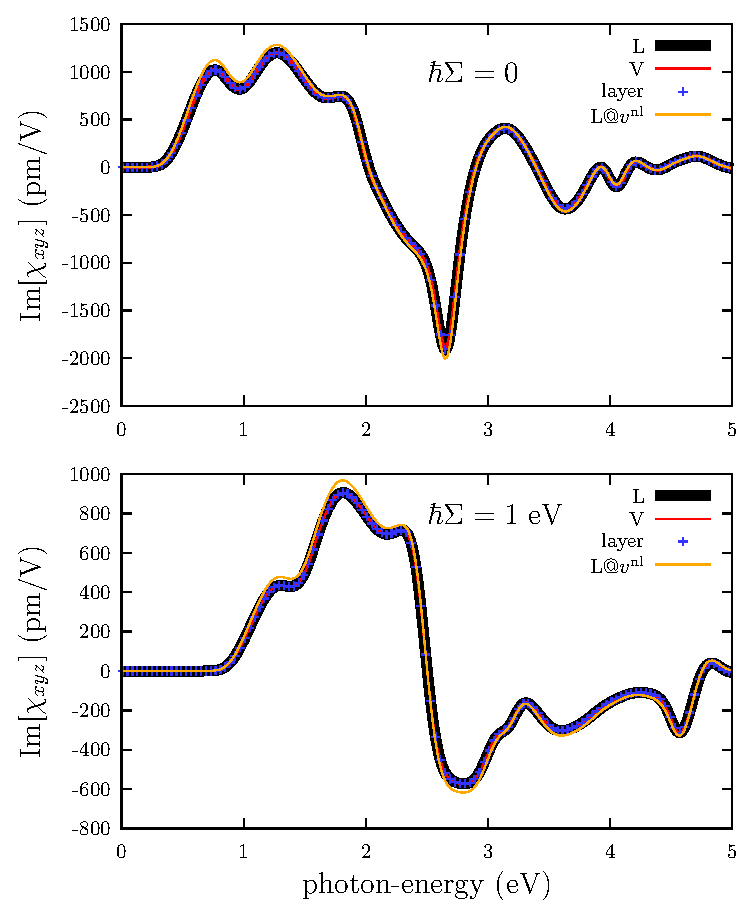
\includegraphics[scale=.7]{figures/plots/shg-bulk}
\caption{Im[$\chi_{xyz}$] for GaAs, 10 Ha and 47 $\bfk$-points, using
  the layered formulation and mimicking a bulk. 
The correction
  due to $\bfv^\nl$, also agrees with the velocity and the layered
  approach (not shown in the figure for clarity).}
\label{gaas}
\end{figure}


\section{Consistency check-up 2}

In Fig.~\ref{si111as} we show
Im[$\chi_{xx}$] for a surface, where the 
The full-slab result is twice the half-slab
result, with or without $\bfv^\nl$,  as it must be. Also, the scissors
correction rigidly shifts the spectrum by $\hbar\gS$ as it should be.  

\begin{figure}[b]
\centering
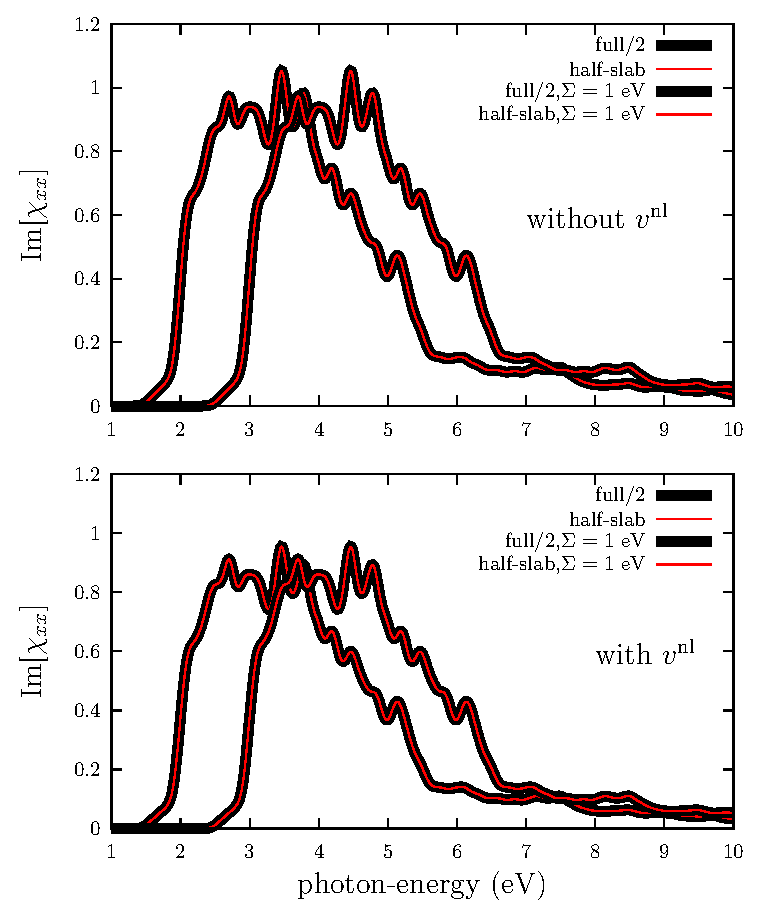
\includegraphics[scale=.7]{figures/plots/surface-chi}
\caption{Im[$\chi_{xx}$] 
for a Si(111):As surface of 6-layers, 5 Ha and 14 $\bfk$-points using
the layered formulation. 
The full-slab result is twice the half-slab
result, as it must be.
}
\label{si111as}
\end{figure}

\section{Consistency check-up 3}

Check-of-Checks: 
A (100) $2\times 1$ surface has $\chi_{xxx}$
 different from zero,
whereas the ideally terminated (100) surface has $\chi_{xxx}=0$.
Clean Si(100) has the $2\times 1$ surface as a possible
reconstruction. Then, to calculate such a surface, one can use
a slab such that its front surface is the reconstructed 
Si(100)$2\times 1$ surface and its back surface is H-terminated.
Therefore,
 for the
layer-by-layer scheme one should expect that
\begin{align}\label{cc3}
\chi^{\mathrm{half-slab}}_{xxx}
\equiv
\chi^{\mathrm{full-slab}}_{xxx}
,
\end{align}
since the contribution from the back surface (H-terminated), would
have zero contribution, since this tensor component of $\chi$ is
symmetry forbidden. Fancy at
Fig.~\ref{si-2x1}, and notice that $\chi^\nl<\chi$. i.e. the
susceptibility with the inclusion of the non-local part of the
pseudopotential is smaller than that without it.\\
King-of-Kings: Rejoice at 
Fig.~\ref{si-2x1-n-vs-b}.
\begin{figure}[b]
\centering 
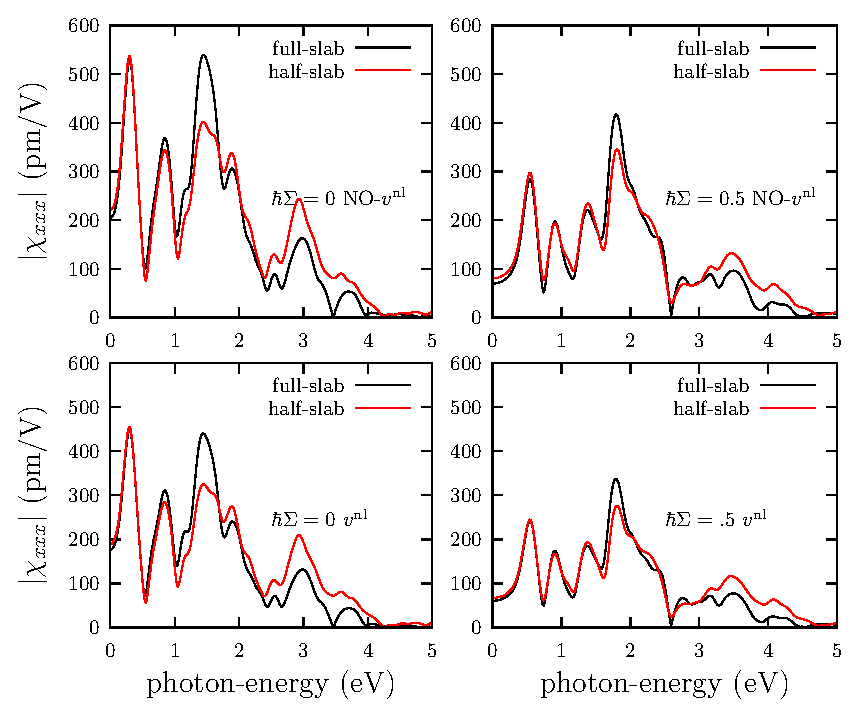
\includegraphics[scale=.7]{figures/plots/shg-si-2x1-16}
\caption{$|\chi_{xxx}|$ 
for a Si(100)$2\times 1$ surface of 16 Si-layers and one H layer, 10 
Ha, 132 bands,  244 $\bfk$-points, and 1000 pwvs in \depe,
 using 
the layered formulation. We see that 
$\chi^{\mathrm{half-slab}}_{xxx}
\sim 
\chi^{\mathrm{full-slab}}_{xxx}$,
validating the layer-by-layer approach. 
}
\label{si-2x1}
\end{figure}
\begin{figure}[b]
\centering
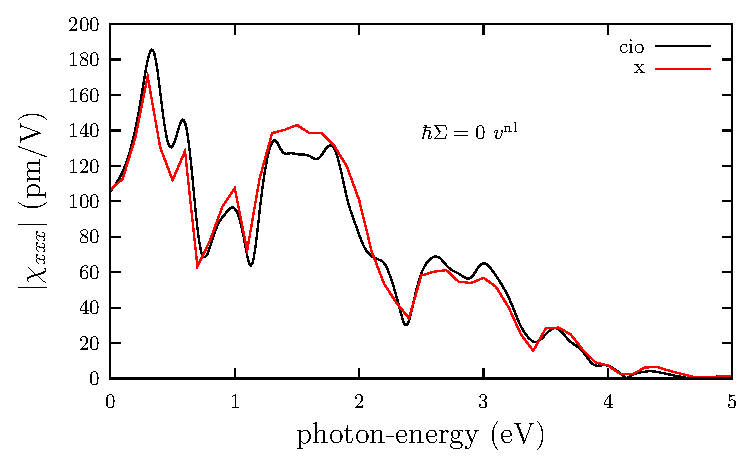
\includegraphics[scale=.7]{figures/plots/shg-si-2x1-n-vs-b}
\caption{$|\chi_{xxx}|$ 
for a Si(100)$2\times 1$ surface of 12 Si-layers and one H layer, 5
Ha, 100 bands and 244 $\bfk$-points for the CIO-\tiniba-coding
and 256 $\bfk$-point for the X-DP\copyr-coding.
Both broadened by 0.1 eV.   
}
\label{si-2x1-n-vs-b}
\end{figure}
\begin{figure}[b]
\centering 
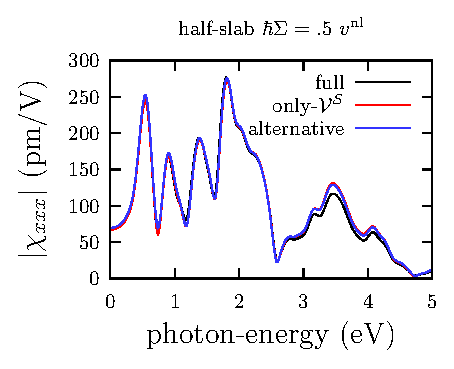
\includegraphics[scale=1.5]{figures/plots/shg-si-2x1-16-compa}
\caption{$|\chi_{xxx}|$ 
for a Si(100)$2\times 1$ surface of 16 Si-layers and one H layer, 10 
Ha, 132 bands, 244 $\bfk$-points and and 1000 pwvs in \depe, using 
the layered formulation. 
``Full'' uses full coding of 
$\calv^\cals_{nm}$ and 
$\calv^\cals_{nm:\bfk}$ through Eq.~\eqref{a.3b};
``only-$\calv^\cals$'' uses 
$\calv^\cals_{nm}$ through Eq.~\eqref{a.3b} and 
$\calv^\cals_{nm:\bfk}$ through Eq.~\eqref{ccu55};
``alternative'' uses $\calv^\cals_{nm}$ through Eq.~\eqref{temp.1} and 
$\calv^\cals_{nm:\bfk}$ through Eq.~\eqref{ccu55}.
Also, we show the results for 2000 pwvs.
Notice that all the curves are almost identical to each other. 
}
\label{si-2x1-compa}
\end{figure}

\section{Consistency check-up 4}\label{ccu4}

To check that the coding of 
$\calc^\ell_{nm}(\bfk)$ 
is correct, we can calculate $\calv^{\rma,\ell}_{nm}(\bfk)$ using
Eq.~\eqref{vcali} as follows
\begin{align}\label{ccu.1}
\calv^{\rma,\ell}_{nm}(\bfk)
&=
\frac{1}{2m_e}
\Big(
\calc^\ell(z)p^\rma
+
p^\rma\calc^\ell(z)
\Big)_{nm}
\nonumber\\
&=
\frac{1}{2m_e}
\sum_q
\Big(
\calc^\ell_{nq}p^\rma_{qm}
+
p^\rma_{nq}\calc^\ell_{qm}
\Big)
,
\end{align}
which must give the same results as those computed through
Eq.~\eqref{eni.2}.
Indeed, we have checked that this is the case. The
\verb=$TINIBA/util/consistency-of-cfmn.sh=
is used to check this.

\section{Consistency check-up 5}\label{ccu5}

When the \verb=-n= option is chosen, using \verb=all_responses.sh= as
coded above doesn't give consistent results, i.e. $\chi$
 with $\bfv^\nl$  
is not smaller than $\chi$ 
 without $\bfv^\nl$. Thus, we follow the bellow approach instead.

We use Eq.~\eqref{nmesn}
\begin{align}\label{nmesnn}
(\calv^{\lda,\rma}_{nm})_{;k^{\rmb}}&=
\frac{\hbar}{m_e}\gd_{\rma\rmb}
C^\ell_{nm} 
-i 
\sum_p 
[r^{\rmb},v^{\nl,\rma}]_{np}C^\ell_{pm} 
+i 
\sum_{\ell}
\bigg(
r^{\rmb}_{n\ell}  
\calv^{\lda,\rma}_{\ell m}
-
\calv^{\lda,\rma}_{n\ell}   
r^{\rmb}_{\ell m}
\bigg)  
+i  
r^{\rmb}_{nm}
\tilde\Delta^{\rma}_{mn}
,
\end{align}  
where 
\begin{eqnarray}\label{tdeln}
\tilde\Delta^{\rma}_{mn}
=
\calv^{\lda,\rma}_{nn}  
-
\calv^{\lda,\rma}_{mm}  
, 
\end{eqnarray}
which is coded instead of Eq.~\eqref{c-a.2nn}. 
 As mentioned before, the term $[r^{\rmb},v^{\nl,\rma}]_{nm}$
calculated in Appendix \ref{calt}, is small 
compared to the other terms, thus we neglect it throwout this work.\cite{valerie} 
The expression for $C^\ell_{nm}$ is calculated in Appendix \ref{calpcalc}.

Likewise, with the help
of Eq.~\eqref{a_gradw2} into
Eq.~\eqref{c-choni.1}, we obain
\begin{align}\label{ccu54}
(v^{\cals,\rma}_{nm})_{;k^\rmb}&=
i\gS f_{mn}(r^\rma_{nm})_{;k^\rmb}
=
i\gS f_{mn}\left(\frac{v^{\lda,\rma}_{nm}}{i\go^\lda_{nm}}\right)_{;k^\rmb}
\nonumber\\
&=
\gS\frac{f_{mn}}{\go^\lda_{nm}}\left[
\left(v^{\lda,a}_{nm}\right)_{;k^\rmb}
-
\frac{v^{\lda,a}_{nm}}{\go^\lda_{nm}}\left(\go^\lda_{nm}\right)_{;k^\rmb}
\right]
\nonumber\\
&=
\gS\frac{f_{mn}}{\go^\lda_{nm}}\left[
\left(v^{\lda,a}_{nm}\right)_{;k^\rmb}
-
\frac{\gD^{b}_{nm}}{\go^\lda_{nm}}v^{\lda,a}_{nm}
\right]
,
\end{align}
which is generalized as follows 
\begin{align}\label{ccu55}
(\calv^{\cals,\rma}_{nm})_{;k^\rmb}&=
\gS\frac{f_{mn}}{\go^\lda_{nm}}\left[
\left(\calv^{\lda,a}_{nm}\right)_{;k^\rmb}
-
\frac{\gD^{b}_{nm}}{\go^\lda_{nm}}\calv^{\lda,a}_{nm}
\right]
,
\end{align}
although, I haven't found a way to prove this rigorously, it gives 
very similar results to those obtained by Eq.~\eqref{c-a.3bnn}, which 
is coded. 
%which is coded instead of 
The following is also tempting,
\begin{align}\label{temp.1}
v^{\cals,a}_{nm}
&=\gS\frac{f_{mn}}{\go^\lda_{nm}}
v^{\lda,a}_{nm}
\nonumber\\
\calv^{\cals,a}_{nm}
&=\gS\frac{f_{mn}}{\go^\lda_{nm}}
\calv^{\lda,a}_{nm}
.
\end{align}
Again, I haven't found a way to prove this rigorously, but it gives 
very similar results to those obtained by Eq.~\eqref{a.3b}, which 
is coded. In Fig.~\ref{si-2x1-compa} we show the comparison between
the two alternatives, from where we see that they are basically equivalent. 



\section{Subroutines}

The following subroutines/shells are involved in the coding,
and are documented between\\
\verb=#BMSd=\\
$\vdots$\\
\verb=#BMSu=\\
marks.
\begin{enumerate}
\item \verb=$TINIBA/utils/all_responses.sh=
\item \verb=$TINIBA/latm/SRC_1setinput/inparams.f90=\\
\textcolor{red}{Warning:} compile both\\
\verb=$TINIBA/latm/SRC_1setinput/= \\
and\\
\verb=$TINIBA/latm/SRC_2latm/= 
\item \verb=$TINIBA/latm/SRC_1setinput/set_input_ascii.f90=\\
\end{enumerate}

\section{Scissors renormalization for $\calv^\gS_{nm}$}\label{voila}

\begin{align}\label{cdg.1}
\bra{n\bfk}\calc(z)\bfr\ket{m\bfk}(E^\gS_m-E^\gS_n) 
&=
\int d\bfr\,\psi^*_{n\bfk}(\bfr) 
\calc(z)\bfr (E^\gS_m-E^\gS_n) 
\psi_{m\bfk}(\bfr) 
\nonumber\\
&=
\int d\bfr\,\psi^*_{n\bfk}(\bfr) 
\calc(z)[\bfr,H^\gS]
\psi_{m\bfk}(\bfr) 
\nonumber\\
&=
-i\int d\bfr\,\psi^*_{n\bfk}(\bfr) 
\calc(z)\bfv^\gS 
\psi_{m\bfk}(\bfr) 
\to 
\calbv^\gS_{nm}
\nonumber\\
\bra{n\bfk}\calc(z)\bfr\ket{m\bfk}
&\to 
\frac{\calbv^\gS_{nm}}{\go^\gS_{nm}}
\nonumber\\
\bra{n\bfk}\calc(z)\bfr\ket{m\bfk}(E^\lda_m-E^\lda_n) 
&=
\int d\bfr\,\psi^*_{n\bfk}(\bfr) 
\calc(z)\bfr (E^\lda_m-E^\lda_n) 
\psi_{m\bfk}(\bfr) 
\nonumber\\
&=
\int d\bfr\,\psi^*_{n\bfk}(\bfr) 
\calc(z)[\bfr,H^\lda]
\psi_{m\bfk}(\bfr) 
\nonumber\\
&=
-i\int d\bfr\,\psi^*_{n\bfk}(\bfr) 
\calc(z)\bfv^\lda 
\psi_{m\bfk}(\bfr) 
\to 
\calbv^\lda_{nm}
\nonumber\\
\bra{n\bfk}\calc(z)\bfr\ket{m\bfk}
&\to 
\frac{\calbv^\lda_{nm}}{\go^\lda_{nm}}
\nonumber\\
\calbv^\gS_{nm}
&=
\frac{\go^\gS_{nm}}{\go^\lda_{nm}}
\calbv^\lda_{nm}\quad{\mathrm{voila}!!!}
.
\end{align}
%code I
\chapter{Divergence Free Expressions for $\chi^s_{\rma\rmb\rmc}$}

We add the $\bfk$ and $-\bfk$ terms of expressions \eqref{pfe} and
\eqref{pfi} to obtain:
\begin{align}\label{chi1}
A
\left[
-\frac{1}{2\go_{lm}(2\go_{lm}-\go_{nm})}\frac{1}{\go_{lm}-\go}
\right]&=-\frac{f_{ml}}{2}
\left[
\frac{{\cal P}^{\rma}_{mn}r^{\rmc}_{nl}r^{\rmb}_{lm}}{\go_{lm}(2\go_{lm}-\go_{nm})}\frac{1}{\go_{lm}-\go}|_{\bfk}
\right.
\nonumber\\
+
\left.
\frac{{\cal P}^{\rma}_{mn}r^{\rmc}_{nl}r^{\rmb}_{lm}}{\go_{lm}(2\go_{lm}-\go_{nm})}\frac{1}{\go_{lm}-\go}|_{-\bfk}
\right]
&=-\frac{f_{ml}}{2}
\left[
\frac{{\cal P}^{\rma}_{mn}r^{\rmc}_{nl}r^{\rmb}_{lm}}{\go_{lm}(2\go_{lm}-\go_{nm})}\frac{1}{\go_{lm}-\go}|_{\bfk}
\right.
\nonumber\\
-
\left.
\frac{{\cal P}^{\rma}_{nm}r^{\rmc}_{ln}r^{\rmb}_{ml}}{\go_{lm}(2\go_{lm}-\go_{nm})}\frac{1}{\go_{lm}-\go}|_{\bfk}
\right]
&=-\frac{f_{ml}}{2}
\frac{1}{\go_{lm}(2\go_{lm}-\go_{nm})}\frac{1}{\go_{lm}-\go}
\nonumber\\
&\times&
\left[
{\cal P}^{\rma}_{mn}r^{\rmc}_{nl}r^{\rmb}_{lm}
-
{\cal P}^{\rma}_{nm}r^{\rmc}_{ln}r^{\rmb}_{ml}
\right]
\\
=-\frac{f_{ml}}{2}
\frac{1}{\go_{lm}(2\go_{lm}-\go_{nm})}\frac{1}{\go_{lm}-\go}
\left[
{\cal P}^{\rma}_{mn}r^{\rmc}_{nl}r^{\rmb}_{lm}
-
({\cal P}^{\rma}_{mn}r^{\rmc}_{nl}r^{\rmb}_{lm})^*
\right]
&=-\frac{f_{ml}}{2}
\frac{2i\mathrm{Im}[{\cal P}^{\rma}_{mn}r^{\rmc}_{nl}r^{\rmb}_{lm}]}{\go_{lm}(2\go_{lm}-\go_{nm})}\frac{1}{\go_{lm}-\go}
\nonumber
,
\end{align}
where we used the Hermiticity of the momentum and position operators.
Likewise we get that
\begin{align}\label{si}
A
\left[
\frac{2}{\go_{nm}(2\go_{lm}-\go_{nm})}\frac{1}{\go_{nm}-2\go}
\right]&=
f_{ml}
\frac{4i\mathrm{Im}[{\cal P}^{\rma}_{mn}r^{\rmc}_{nl}r^{\rmb}_{lm}]}{\go_{nm}(2\go_{lm}-\go_{nm})}\frac{1}{\go_{nm}-2\go}
.
\end{align}
Also,
\begin{align}\label{is}
&-
f_{ln}{\cal P}^{\rma}_{mn}r^{\rmb}_{nl}r^{\rmc}_{lm}
\left[
-\frac{1}{2\go_{nl}(2\go_{nl}-\go_{nm})}\frac{1}{\go_{nl}-\go}
+\frac{2}{\go_{nm}(2\go_{nl}-\go_{nm})}\frac{1}{\go_{nm}-2\go}
\right]
\nonumber\\
&=
-
2if_{ln}\mathrm{Im}[{\cal P}^{\rma}_{mn}r^{\rmb}_{nl}r^{\rmc}_{lm}]
\left[
-\frac{1}{2\go_{nl}(2\go_{nl}-\go_{nm})}\frac{1}{\go_{nl}-\go}
+\frac{2}{\go_{nm}(2\go_{nl}-\go_{nm})}\frac{1}{\go_{nm}-2\go}
\right]
,
\end{align}
and therefore
\begin{align}\label{pfen}  
E&=  
2if_{ml}\mathrm{Im}[{\cal P}^{\rma}_{mn}r^{\rmc}_{nl}r^{\rmb}_{lm}] 
\left[
-\frac{1}{2\go_{lm}(2\go_{lm}-\go_{nm})}\frac{1}{\go_{lm}-\go}
+\frac{2}{\go_{nm}(2\go_{lm}-\go_{nm})}\frac{1}{\go_{nm}-2\go}
\right]
\nonumber\\
&- 
2if_{ln}\mathrm{Im}[{\cal P}^{\rma}_{mn}r^{\rmb}_{nl}r^{\rmc}_{lm}]
\left[
-\frac{1}{2\go_{nl}(2\go_{nl}-\go_{nm})}\frac{1}{\go_{nl}-\go}
+\frac{2}{\go_{nm}(2\go_{nl}-\go_{nm})}\frac{1}{\go_{nm}-2\go}
\right]
.
\end{align}  
Using above results into Eq.~\eqref{chie} implies
\begin{align}\label{pfen3} 
\chi_{e,\rma\rmb\rmc}^{s,\ell}
&= 
-\frac{2e^3}{m_e\hbar^2} 
\sum_{\ell m n\bfk}
\left[ 
f_{ml}\mathrm{Im}[{\cal P}^{\rma}_{mn}r^{\rmc}_{nl}r^{\rmb}_{lm}] 
\left[
-\frac{1}{2\go_{lm}(2\go_{lm}-\go_{nm})}\frac{1}{\go_{lm}-\go}
+\frac{2}{\go_{nm}(2\go_{lm}-\go_{nm})}\frac{1}{\go_{nm}-2\go}
\right]
\right.
\nonumber\\
&-
\left. 
f_{ln}\mathrm{Im}[{\cal P}^{\rma}_{mn}r^{\rmb}_{nl}r^{\rmc}_{lm}]
\left[
-\frac{1}{2\go_{nl}(2\go_{nl}-\go_{nm})}\frac{1}{\go_{nl}-\go}
+\frac{2}{\go_{nm}(2\go_{nl}-\go_{nm})}\frac{1}{\go_{nm}-2\go}
\right]
\right]
\nonumber\\
&= 
-\frac{2e^3}{m_e\hbar^2} 
\sum_{\ell m n\bfk}
\left[ 
f_{ml}\mathrm{Im}[{\cal P}^{\rma}_{mn}\{r^{\rmc}_{nl}r^{\rmb}_{lm}\}] 
\left[
-\frac{1}{2\go_{lm}(2\go_{lm}-\go_{nm})}\frac{1}{\go_{lm}-\go}
+\frac{2}{\go_{nm}(2\go_{lm}-\go_{nm})}\frac{1}{\go_{nm}-2\go}
\right]
\right.
\nonumber\\
&-
\left. 
f_{ln}\mathrm{Im}[{\cal P}^{\rma}_{mn}\{r^{\rmb}_{nl}r^{\rmc}_{lm}\}]
\left[
-\frac{1}{2\go_{nl}(2\go_{nl}-\go_{nm})}\frac{1}{\go_{nl}-\go}
+\frac{2}{\go_{nm}(2\go_{nl}-\go_{nm})}\frac{1}{\go_{nm}-2\go}
\right]
\right]
,
\end{align}  
where $\{\}$ is the symmetrization of the Cartesian indices $\rmb\rmc$, i.e. 
$\{u^{\rmb}s^{\rmc}\}=(u^{\rmb}s^{\rmc}+u^{\rmc}s^{\rmb})/2$. 
Then, we see that
$\chi_{e,\rma\rmb\rmc}^{s,\ell}=\chi_{e,acb}^{s,\ell}$. We further simplify 
the last equation as follows:
\begin{align}\label{pfen2} 
\chi_{e,\rma\rmb\rmc}^{s,\ell}
&= 
-\frac{2e^3}{2m_e\hbar^2} 
\sum_{\ell m n\bfk}
\left[
\left[
-\frac{f_{ml}\mathrm{Im}[{\cal P}^{\rma}_{mn}\{r^{\rmc}_{nl}r^{\rmb}_{lm}\}]}
{2\go_{lm}(2\go_{lm}-\go_{nm})}\frac{1}{\go_{lm}-\go}
+\frac{2 f_{ml}\mathrm{Im}[{\cal P}^{\rma}_{mn}\{r^{\rmc}_{nl}r^{\rmb}_{lm}\}]}
{\go_{nm}(2\go_{lm}-\go_{nm})}\frac{1}{\go_{nm}-2\go}
\right]
\right.
\nonumber\\
&+
\left.
\left[
\frac{f_{ln}\mathrm{Im}[{\cal P}^{\rma}_{mn}\{r^{\rmb}_{nl}r^{\rmc}_{lm}\}]}
{2\go_{nl}(2\go_{nl}-\go_{nm})}\frac{1}{\go_{nl}-\go}
-\frac{2 f_{ln}\mathrm{Im}[{\cal P}^{\rma}_{mn}\{r^{\rmb}_{nl}r^{\rmc}_{lm}\}]
}{\go_{nm}(2\go_{nl}-\go_{nm})}\frac{1}{\go_{nm}-2\go}
\right]
\right]
\nonumber\\
&=
-\frac{2e^3}{m_e\hbar^2} 
\sum_{\ell m n\bfk}
\left[
\left[
\frac{2 f_{ml}\mathrm{Im}[{\cal P}^{\rma}_{mn}\{r^{\rmc}_{nl}r^{\rmb}_{lm}\}]}
{\go_{nm}(2\go_{lm}-\go_{nm})}
-\frac{2 f_{ln}\mathrm{Im}[{\cal P}^{\rma}_{mn}\{r^{\rmb}_{nl}r^{\rmc}_{lm}\}]
}{\go_{nm}(2\go_{nl}-\go_{nm})}
\right]
\frac{1}{\go_{nm}-2\go}
\right.
\nonumber\\
&+
\left.
\left[
\frac{f_{ln}\mathrm{Im}[{\cal P}^{\rma}_{mn}\{r^{\rmb}_{nl}r^{\rmc}_{lm}\}]}
{2\go_{nl}(2\go_{nl}-\go_{nm})}\frac{1}{\go_{nl}-\go}
-\frac{f_{ml}\mathrm{Im}[{\cal P}^{\rma}_{mn}\{r^{\rmc}_{nl}r^{\rmb}_{lm}\}]}
{2\go_{lm}(2\go_{lm}-\go_{nm})}
\frac{1}{\go_{lm}-\go}|_{\ell\leftrightarrow m}
\right]
\right]
\nonumber\\
&=
-\frac{e^3}{m_e\hbar^2} 
\sum_{\ell m n\bfk}
\left[
\left[
\frac{2 f_{ml}\mathrm{Im}[{\cal P}^{\rma}_{mn}\{r^{\rmc}_{nl}r^{\rmb}_{lm}\}]}
{\go_{nm}(2\go_{lm}-\go_{nm})}
-\frac{2 f_{ln}\mathrm{Im}[{\cal P}^{\rma}_{mn}\{r^{\rmb}_{nl}r^{\rmc}_{lm}\}]
}{\go_{nm}(2\go_{nl}-\go_{nm})}
\right]
\frac{1}{\go_{nm}-2\go}
\right.
\nonumber\\
&+
\left.
\left[
\frac{f_{ln}\mathrm{Im}[{\cal P}^{\rma}_{mn}\{r^{\rmb}_{nl}r^{\rmc}_{lm}\}]}
{2\go_{nl}(2\go_{nl}-\go_{nm})}\frac{1}{\go_{nl}-\go}
-\frac{f_{lm}\mathrm{Im}[{\cal P}^{\rma}_{ln}\{r^{\rmc}_{nm}r^{\rmb}_{ml}\}]}
{2\go_{ml}(2\go_{ml}-\go_{nl})}\frac{1}{\go_{ml}-\go}|_{n\leftrightarrow m}
\right]
\right]
\nonumber\\
&=
-\frac{e^3}{m_e\hbar^2} 
\sum_{\ell m n\bfk}
\left[
\left[
\frac{2 f_{ml}\mathrm{Im}[{\cal P}^{\rma}_{mn}\{r^{\rmc}_{nl}r^{\rmb}_{lm}\}]}
{\go_{nm}(2\go_{lm}-\go_{nm})}
-\frac{2 f_{ln}\mathrm{Im}[{\cal P}^{\rma}_{mn}\{r^{\rmb}_{nl}r^{\rmc}_{lm}\}]
}{\go_{nm}(2\go_{nl}-\go_{nm})}
\right]
\frac{1}{\go_{nm}-2\go}
\right.
\nonumber\\
&+
\left.
\left[
\frac{f_{ln}\mathrm{Im}[{\cal P}^{\rma}_{mn}\{r^{\rmb}_{nl}r^{\rmc}_{lm}\}]}
{2\go_{nl}(2\go_{nl}-\go_{nm})}\frac{1}{\go_{nl}-\go}
-\frac{f_{ln}\mathrm{Im}[{\cal P}^{\rma}_{lm}\{r^{\rmc}_{mn}r^{\rmb}_{nl}\}]}
{2\go_{nl}(2\go_{nl}-\go_{ml})}\frac{1}{\go_{nl}-\go}
\right]
\right]
\nonumber\\
&=
-\frac{e^3}{m_e\hbar^2} 
\sum_{\ell m n\bfk}
\left[
\left[
\frac{2 f_{ml}\mathrm{Im}[{\cal P}^{\rma}_{mn}\{r^{\rmc}_{nl}r^{\rmb}_{lm}\}]}
{\go_{nm}(2\go_{lm}-\go_{nm})}
-\frac{2 f_{ln}\mathrm{Im}[{\cal P}^{\rma}_{mn}\{r^{\rmb}_{nl}r^{\rmc}_{lm}\}]
}{\go_{nm}(2\go_{nl}-\go_{nm})}
\right]
\frac{1}{\go_{nm}-2\go}
\right.
\nonumber\\
&+
\left. 
f_{ln}
\left[
\frac{\mathrm{Im}[{\cal P}^{\rma}_{mn}\{r^{\rmb}_{nl}r^{\rmc}_{lm}\}]}
{2\go_{nl}(2\go_{nl}-\go_{nm})}
-\frac{f_{ln}\mathrm{Im}[{\cal P}^{\rma}_{lm}\{r^{\rmc}_{mn}r^{\rmb}_{nl}\}]}
{2\go_{nl}(2\go_{nl}-\go_{ml})}
\right]\frac{1}{\go_{nl}-\go}
\right]
,
\end{align}  
where the 2 in the denominator of the prefactor after the first equal
sign comes from the $\bfk$ and $-\bfk$ addition, i.e. 
$\chi\to\sum_{\bfk>0}[\chi(\bfk)+\chi(-\bfk)]/2$. 
Taking $\go\to\go +i\eta$ and use
$\lim_{\eta\to 0}1/(x-i\eta)=P(1/x)+i\pi\gd(x)$, to get
\begin{align}\label{imchie}
\mathrm{Im}[\chi_{e,\rma\rmb\rmc}^{s,\ell}]
&=
\frac{2\pi e^3}{m_e\hbar^2} 
\sum_{\ell m n\bfk}
\left[
\left[
\frac{2 f_{ln}\mathrm{Im}[{\cal P}^{\rma}_{mn}\{r^{\rmb}_{nl}r^{\rmc}_{lm}\}]
}{\go_{nm}(2\go_{nl}-\go_{nm})}
-\frac{2 f_{ml}\mathrm{Im}[{\cal P}^{\rma}_{mn}\{r^{\rmc}_{nl}r^{\rmb}_{lm}\}]}
{\go_{nm}(2\go_{lm}-\go_{nm})}
\right]
\gd(\go_{nm}-2\go)
\right.
\nonumber\\
&+
\left. 
f_{ln}
\left[
\frac{\mathrm{Im}[{\cal P}^{\rma}_{lm}\{r^{\rmc}_{mn}r^{\rmb}_{nl}\}]}
{2\go_{nl}(2\go_{nl}-\go_{ml})}
-
\frac{\mathrm{Im}[{\cal P}^{\rma}_{mn}\{r^{\rmb}_{nl}r^{\rmc}_{lm}\}]}
{2\go_{nl}(2\go_{nl}-\go_{nm})}
\right]
\gd(\go_{nl}-\go)
\right]
.
\end{align}  
We change $l\leftrightarrow m$ in the last term,
to write
\begin{align}\label{imchie2}
\mathrm{Im}[\chi_{e,\rma\rmb\rmc}^{s,\ell}]
&=
\frac{\pi e^3}{m_e\hbar^2} 
\sum_{\ell m n\bfk}
\left[
\left[
\frac{2 f_{ln}\mathrm{Im}[{\cal P}^{\rma}_{mn}\{r^{\rmb}_{nl}r^{\rmc}_{lm}\}]
}{\go_{nm}(2\go_{nl}-\go_{nm})}
-\frac{2 f_{ml}\mathrm{Im}[{\cal P}^{\rma}_{mn}\{r^{\rmc}_{nl}r^{\rmb}_{lm}\}]}
{\go_{nm}(2\go_{lm}-\go_{nm})}
\right]
\gd(\go_{nm}-2\go)
\right.
\nonumber\\
&+
\left. 
f_{mn}
\left[
\frac{\mathrm{Im}[{\cal P}^{\rma}_{ml}\{r^{\rmc}_{ln}r^{\rmb}_{nm}\}]}
{2\go_{nm}(2\go_{nm}-\go_{lm})}
-
\frac{\mathrm{Im}[{\cal P}^{\rma}_{ln}\{r^{\rmb}_{nm}r^{\rmc}_{ml}\}]}
{2\go_{nm}(2\go_{nm}-\go_{nl})}
\right]
\gd(\go_{nm}-\go)
\right]
.
\end{align}  
From the delta functions it follows that $n=c$ and $m=v$, then
$f_{ln}=1$ with $l=v'$,
$f_{ml}=1$ with $l=c'$, 
and
$f_{mn}=1$ with $l=c'$ or $v'$, and
\begin{align}\label{imchie3}
\mathrm{Im}[\chi_{e,\rma\rmb\rmc}^{s,\ell}]
&=
\frac{\pi e^3}{m_e\hbar^2} 
\sum_{vc\bfk}
\left[
\left[
\sum_{v'\ne v}
\frac{2\mathrm{Im}[{\cal P}^{\rma,\ell}_{vc}\{r^{\rmb}_{cv'}r^{\rmc}_{v'v}\}]
}{\go_{cv}(2\go_{cv'}-\go_{cv})}
-
\sum_{c'\ne c}
\frac{2\mathrm{Im}[{\cal P}^{\rma,\ell}_{vc}\{r^{\rmc}_{cc'}r^{\rmb}_{c'v}\}]}
{\go_{cv}(2\go_{c'v}-\go_{cv})}
\right]
\gd(\go_{cv}-2\go)
\right.
\nonumber\\
&+
\left.
\sum_{l\neq(v,c)}
\left[
\frac{\mathrm{Im}[{\cal P}^{\rma,\ell}_{vl}\{r^{\rmc}_{lc}r^{\rmb}_{cv}\}]}
{2\go_{cv}(2\go_{cv}-\go_{lv})}
-
\frac{\mathrm{Im}[{\cal P}^{\rma,\ell}_{lc}\{r^{\rmb}_{cv}r^{\rmc}_{vl}\}]}
{2\go_{cv}(2\go_{cv}-\go_{cl})}
\right]
\gd(\go_{cv}-\go)
\right]
,
\end{align}  
where we put the layer $\ell$ dependence in ${\cal P}$.
Using Eq.~\eqref{rcal}, we can obtain the following result
\begin{align}\label{ptor}
2i\mathrm{Im}[{\cal P}^{\rma,\ell}_{nm}\{r^{\rmb}_{ml}r^{\rmc}_{ln}\}]
&=
{\cal P}^{\rma,\ell}_{nm}\{r^{\rmb}_{ml}r^{\rmc}_{ln}\}
-
({\cal P}^{\rma,\ell}_{nm}\{r^{\rmb}_{ml}r^{\rmc}_{ln}\})^*
\nonumber\\
&=
im_e\go_{nm}{\cal R}^{\rma,\ell}_{nm}\{r^{\rmb}_{ml}r^{\rmc}_{ln}\}
-
(im_e\go_{nm}{\cal R}^{\rma,\ell}_{nm}\{r^{\rmb}_{ml}r^{\rmc}_{ln}\})^*
\nonumber\\
&=
im_e\go_{nm}\left({\cal R}^{\rma,\ell}_{nm}\{r^{\rmb}_{ml}r^{\rmc}_{ln}\}
+
({\cal R}^{\rma,\ell}_{nm}\{r^{\rmb}_{ml}r^{\rmc}_{ln}\})^*
\right)
\nonumber\\
&=
2im_e\go_{nm}\mathrm{Re}[{\cal R}^{\rma,\ell}_{nm}\{r^{\rmb}_{ml}r^{\rmc}_{ln}\}]
,
\end{align}
then, using $\go_{vc}=-\go_{vc}$ we obtain
\begin{align}\label{imchie3n}
\mathrm{Im}[\chi_{e,\rma\rmb\rmc}^{s,\ell}]
&=
\frac{\pi e^3}{\hbar^2} 
\sum_{vc\bfk}
\left[
\left[
-\sum_{v'\ne v}
\frac{2\mathrm{Re}[{\cal R}^{\rma,\ell}_{vc}\{r^{\rmb}_{cv'}r^{\rmc}_{v'v}\}]
}{2\go_{cv'}-\go_{cv}}
+
\sum_{c'\ne c}
\frac{2\mathrm{Re}[{\cal R}^{\rma,\ell}_{vc}\{r^{\rmc}_{cc'}r^{\rmb}_{c'v}\}]}
{2\go_{c'v}-\go_{cv}}
\right]
\gd(\go_{cv}-2\go)
\right.
\nonumber\\
&+
\left.
\sum_{l\neq(v,c)}
\left[
\frac{\go_{vl}\mathrm{Re}[{\cal R}^{\rma,\ell}_{vl}\{r^{\rmc}_{lc}r^{\rmb}_{cv}\}]}
{2\go_{cv}(2\go_{cv}-\go_{lv})}
-
\frac{\go_{lc}\mathrm{Re}[{\cal R}^{\rma,\ell}_{lc}\{r^{\rmb}_{cv}r^{\rmc}_{vl}\}]}
{2\go_{cv}(2\go_{cv}-\go_{cl})}
\right]
\gd(\go_{cv}-\go)
\right]
.
\end{align}  
Finally, following Ref.~\cite{nastos_scissors_2005,cabellos_effects_2009} we simply change
$\go_{nm}\to\go_{nm}^S$ to obtain the scissored expresion of
\begin{align}\label{imchies}
\mathrm{Im}[\chi_{e,\rma\rmb\rmc}^{s,\ell}]
&=
\frac{\pi e^3}{2\hbar^2} 
\sum_{vc\bfk}
\left[
4
\left[
-\sum_{v'\ne v}
\frac{\mathrm{Re}[{\cal R}^{\rma,\ell}_{vc}\{r^{\rmb}_{cv'}r^{\rmc}_{v'v}\}]
}{2\go^S_{cv'}-\go^S_{cv}}
+
\sum_{c'\ne c}
\frac{\mathrm{Re}[{\cal R}^{\rma,\ell}_{vc}\{r^{\rmc}_{cc'}r^{\rmb}_{c'v}\}]}
{2\go^S_{c'v}-\go^S_{cv}}
\right]
\gd(\go^S_{cv}-2\go)
\right.
\nonumber\\
&+
\left.
\sum_{l\neq(v,c)}
\left[
\frac{\go^S_{vl}\mathrm{Re}[{\cal R}^{\rma,\ell}_{vl}\{r^{\rmc}_{lc}r^{\rmb}_{cv}\}]}
{\go^S_{cv}(2\go^S_{cv}-\go^S_{lv})}
-
\frac{\go^S_{lc}\mathrm{Re}[{\cal R}^{\rma,\ell}_{lc}\{r^{\rmb}_{cv}r^{\rmc}_{vl}\}]}
{\go^S_{cv}(2\go^S_{cv}-\go^S_{cl})}
\right]
\gd(\go^S_{cv}-\go)
\right]
,
\end{align}  
where we have ``pulled'' a factor of 1/2, so the prefactor is the same
as that of the velocity gauge formalism.\cite{cabellos_effects_2009} 
For the $I$ term of Eq.~\eqref{pfi}, we notice that the energy
denominators are invariant under $\bfk\to -\bfk$, and then we only
look at the numerators, then
\begin{align}\label{ct}
C\to f_{mn}{\cal P}^{\rma}_{mn}(r^{\rmb}_{nm})_{;k^{\rmc}}|_{\bfk}
+
f_{mn}{\cal P}^{\rma}_{mn}(r^{\rmb}_{nm})_{;k^{\rmc}}|_{-\bfk}
&=
f_{mn}\left[{\cal P}^{\rma}_{mn}(r^{\rmb}_{nm})_{;k^{\rmc}}|_{\bfk}
+
(-{\cal P}^{\rma}_{nm})(-(r^{\rmb}_{mn})_{;k^{\rmc}})|_{\bfk}
\right]
\nonumber\\
&=
f_{mn}\left[{\cal P}^{\rma}_{mn}(r^{\rmb}_{nm})_{;k^{\rmc}}
+
{\cal P}^{\rma}_{nm}(r^{\rmb}_{mn})_{;k^{\rmc}}
\right]
\nonumber\\
&=
f_{mn}\left[{\cal P}^{\rma}_{mn}(r^{\rmb}_{nm})_{;k^{\rmc}}
+
({\cal P}^{\rma}_{mn}(r^{\rmb}_{nm})_{;k^{\rmc}})^*
\right]
\nonumber\\
&= 
m_ef_{mn}\go_{mn}\left[i{\cal R}^{\rma}_{mn}(r^{\rmb}_{nm})_{;k^{\rmc}}
+
(i{\cal R}^{\rma}_{mn}(r^{\rmb}_{nm})_{;k^{\rmc}})^*
\right]
\nonumber\\
&= 
im_ef_{mn}\go_{mn}\left[{\cal R}^{\rma}_{mn}(r^{\rmb}_{nm})_{;k^{\rmc}}
-
({\cal R}^{\rma}_{mn}(r^{\rmb}_{nm})_{;k^{\rmc}})^*
\right]
\nonumber\\
&= 
-2m_ef_{mn}\go_{mn}\mathrm{Im}[{\cal R}^{\rma}_{mn}(r^{\rmb}_{nm})_{;k^{\rmc}}]
,
\end{align}
with similar results for 
$D=-2f_{mn}\go_{mn}\mathrm{Im}[{\cal  R}^{\rma}_{mn}r^{\rmb}_{nm}]\gD^{\rmc}_{nm}$.
 Now, from Eq.~\eqref{chr}, we obtain
that the first term reduces to
\begin{align}\label{chrn2}
\frac{r^{\rmb}_{nm}}{\go_{nm}}\left({\cal R}^{\rma}_{mn}\right)_{;k^{\rmc}}|_{\bfk}
+
\frac{r^{\rmb}_{nm}}{\go_{nm}}\left({\cal R}^{\rma}_{mn}\right)_{;k^{\rmc}}|_{-\bfk}
&=
\frac{r^{\rmb}_{nm}}{\go_{nm}}\left({\cal R}^{\rma}_{mn}\right)_{;k^{\rmc}}|_{\bfk}
-
\frac{r^{\rmb}_{mn}}{\go_{nm}}\left({\cal R}^{\rma}_{nm}\right)_{;k^{\rmc}}|_{\bfk}
\nonumber\\
&=
\frac{1}{\go_{nm}}\left[r^{\rmb}_{nm}\left({\cal R}^{\rma}_{mn}\right)_{;k^{\rmc}}
-
(r^{\rmb}_{nm}\left({\cal R}^{\rma}_{mn}\right)_{;k^{\rmc}})^*\right]
\nonumber\\
&=
\frac{2i}{\go_{nm}}\mathrm{Im}[r^{\rmb}_{nm}\left({\cal R}^{\rma}_{mn}\right)_{;k^{\rmc}}]
,
\end{align}
with similar results for the other two terms. First, we collect the
$2\go$ terms form Eq.~\eqref{pfi} that contribute to Eq.~\eqref{chii}
\begin{align}\label{2wchii}
I_{2\go}&=
-\frac{e^3}{2\hbar^2}\sum_{mn\bfk}
\left[
\frac{-4f_{mn}\go_{mn}\mathrm{Im}[{\cal R}^{\rma}_{mn}\left(r^{\rmb}_{nm}\right)_{;k^{\rmc}}]}{\go^2_{nm}}
-
\frac{-8f_{mn}\go_{mn}\mathrm{Im}[{\cal R}^{\rma}_{mn}r^{\rmb}_{nm}]\gD^{\rmc}_{nm}}{\go^3_{nm}}
\right]\frac{1}{\go_{nm}-2\go}
\nonumber\\
&=
\frac{e^3}{2\hbar^2}\sum_{mn\bfk}
\left[
\frac{4f_{mn}\go_{mn}\mathrm{Im}[{\cal R}^{\rma}_{mn}\left(r^{\rmb}_{nm}\right)_{;k^{\rmc}}]}{\go^2_{nm}}
-
\frac{8f_{mn}\go_{mn}\mathrm{Im}[{\cal R}^{\rma}_{mn}r^{\rmb}_{nm}]\gD^{\rmc}_{nm}}{\go^3_{nm}}
\right]\frac{1}{\go_{nm}-2\go}
\nonumber\\
&=
\frac{e^3}{2\hbar^2}\sum_{mn\bfk}
\left[
\frac{-4f_{mn}\mathrm{Im}[{\cal R}^{\rma}_{mn}\left(r^{\rmb}_{nm}\right)_{;k^{\rmc}}]}{\go_{nm}}
+
\frac{8f_{mn}\mathrm{Im}[{\cal R}^{\rma}_{mn}r^{\rmb}_{nm}]\gD^{\rmc}_{nm}}{\go^2_{nm}}
\right]\frac{1}{\go_{nm}-2\go}
,
\end{align}
where the 2 in the denominator of the prefactor
comes from the $\bfk$ and $-\bfk$ addition, as previously noted.
Taking $\eta\to 0$ we get that
\begin{align}\label{imchi2w}
\mathrm{Im}[\chi_{i,\rma\rmb\rmc,2\go}^{s,\ell}]
&=
\frac{\pi|e|^3}{2\hbar^2}\sum_{mn\bfk}
\frac{4f_{mn}}{\go_{nm}}
\left[
\mathrm{Im}[{\cal R}^{\rma}_{mn}\left(r^{\rmb}_{nm}\right)_{;k^{\rmc}}]
-
\frac{2\mathrm{Im}[{\cal R}^{\rma}_{mn}r^{\rmb}_{nm}]\gD^{\rmc}_{nm}}{\go_{nm}}
\right]\gd(\go_{nm}-2\go)
\nonumber \\
&=
\frac{\pi|e|^3}{2\hbar^2}\sum_{vc\bfk}
\frac{4}{\go^S_{cv}}
\left[
\mathrm{Im}[{\cal R}^{\rma,\ell}_{vc}\{\left(r^{\rmb}_{cv}\right)_{;k^{\rmc}}\}]
-
\frac{2\mathrm{Im}[{\cal R}^{\rma,\ell}_{vc}\{r^{\rmb}_{cv}]\gD^{\rmc}_{cv}\}}{\go^S_{cv}}
\right]\gd(\go^S_{cv}-2\go)
,
\end{align} 
where from the delta term we must have $n=c$ and $m=v$. The expression
is symmetric in the last two indices and is properly scissor shifted
as well. 

The $\go$ terms are
\begin{align}\label{pfia}
I_{\go}
&=
-\frac{e^3}{m_e2\hbar^2}
\sum_{nm\bfk}
\left[
\left[
-\frac{C}{2\go^2_{nm}}
+
\frac{3D}{2\go^3_{nm}}
\right]\frac{1}{\go_{nm}-\go}
+
\frac{D}{2\go^2_{nm}}\frac{1}{(\go_{nm}-\go)^2}
\right]
\nonumber\\
&=
-\frac{e^3}{m_e2\hbar^2}
\sum_{nm\bfk}
\left[
\left[
-\frac{-2m_ef_{mn}\go_{mn}\mathrm{Im}[{\cal R}^{\rma}_{mn}(r^{\rmb}_{nm})_{;k^{\rmc}}]
}{2\go^2_{nm}}
+
\frac{3(-2m_ef_{mn}\go_{mn}\mathrm{Im}[{\cal R}^{\rma}_{mn}r^{\rmb}_{nm}]\gD^{\rmc}_{nm})}{2\go^3_{nm}}
\right]\frac{1}{\go_{nm}-\go}
\right.
\nonumber\\
&+
\left.
\frac{-im_ef_{mn}}{2}
\left(
\frac{{\cal R}^{\rma}_{mn}r^{\rmb}_{nm}}{\go_{nm}}
\right)_{;k^{\rmc}}
\frac{1}{\go_{nm}-\go}
\right]
\nonumber\\
&=
\frac{|e|^3}{2\hbar^2}
\sum_{nm\bfk}
f_{mn}
\left[
-\frac{\mathrm{Im}[{\cal R}^{\rma}_{mn}(r^{\rmb}_{nm})_{;k^{\rmc}}]
}{\go_{nm}}
+
\frac{3\mathrm{Im}[{\cal R}^{\rma}_{mn}r^{\rmb}_{nm}]\gD^{\rmc}_{nm}}{\go^2_{nm}}
-
\frac{i}{2}
\left(
\frac{{\cal R}^{\rma}_{mn}r^{\rmb}_{nm}}{\go_{nm}}
\right)_{;k^{\rmc}}
\right]\frac{1}{\go_{nm}-\go}
\nonumber\\
&=
\frac{|e|^3}{2\hbar^2}
\sum_{nm\bfk}
f_{mn}
\left[
-\frac{\mathrm{Im}[{\cal R}^{\rma}_{mn}(r^{\rmb}_{nm})_{;k^{\rmc}}]
}{\go_{nm}}
+
\frac{3\mathrm{Im}[{\cal R}^{\rma}_{mn}r^{\rmb}_{nm}]\gD^{\rmc}_{nm}}{\go^2_{nm}}
-
\frac{i}{2}
\left[
\frac{r^{\rmb}_{nm}}{\go_{nm}}
\left(
{\cal R}^{\rma}_{mn}
\right)_{;k^{\rmc}}
\right.
\right.
\nonumber\\
&+
\left.
\left.
\frac{{\cal R}^{\rma}_{mn}}{\go_{nm}}
\left(
r^{\rmb}_{nm}
\right)_{;k^{\rmc}}
-
\frac{{\cal R}^{\rma}_{mn}r^{\rmb}_{nm}}{\go^2_{nm}}
\left(
\go_{nm}
\right)_{;k^{\rmc}}
\right]
\right]
\frac{1}{\go_{nm}-\go}
\nonumber\\
&=
\frac{|e|^3}{2\hbar^2}
\sum_{nm\bfk}
f_{mn}
\left[
-\frac{\mathrm{Im}[{\cal R}^{\rma}_{mn}(r^{\rmb}_{nm})_{;k^{\rmc}}]
}{\go_{nm}}
+
\frac{3\mathrm{Im}[{\cal R}^{\rma}_{mn}r^{\rmb}_{nm}]\gD^{\rmc}_{nm}}{\go^2_{nm}}
-
\frac{i}{2}
\left[
\frac{2i}{\go_{nm}}
\mathrm{Im}[r^{\rmb}_{nm}\left({\cal R}^{\rma}_{mn}\right)_{;k^{\rmc}}]
\right.
\right.
\nonumber\\
&+
\left.
\left.
\frac{2i}{\go_{nm}}
\mathrm{Im}[
{\cal R}^{\rma}_{mn}
\left(
r^{\rmb}_{nm}
\right)_{;k^{\rmc}}
]
-
\frac{2i}{\go^2_{nm}}
\mathrm{Im}[{\cal R}^{\rma}_{mn}r^{\rmb}_{nm}]
\gD^{\rmc}_{nm}
\right]
\right]
\frac{1}{\go_{nm}-\go}
\nonumber\\
&=
\frac{|e|^3}{2\hbar^2}
\sum_{nm\bfk}
f_{mn}
\left[
-\frac{\mathrm{Im}[{\cal R}^{\rma}_{mn}(r^{\rmb}_{nm})_{;k^{\rmc}}]
}{\go_{nm}}
+
\frac{3\mathrm{Im}[{\cal R}^{\rma}_{mn}r^{\rmb}_{nm}]\gD^{\rmc}_{nm}}{\go^2_{nm}}
+
\frac{1}{\go_{nm}}
\mathrm{Im}[r^{\rmb}_{nm}\left({\cal R}^{\rma}_{mn}\right)_{;k^{\rmc}}]
\right.
\nonumber\\
&+
\left.
\frac{1}{\go_{nm}}
\mathrm{Im}[
{\cal R}^{\rma}_{mn}
\left(
r^{\rmb}_{nm}
\right)_{;k^{\rmc}}
]
-
\frac{1}{\go^2_{nm}}
\mathrm{Im}[{\cal R}^{\rma}_{mn}r^{\rmb}_{nm}]
\gD^{\rmc}_{nm}
\right]
\frac{1}{\go_{nm}-\go}
,
\end{align}
or
\begin{align}\label{pfian}
I_{\go}
&=
\frac{|e|^3}{2\hbar^2}
\sum_{nm\bfk}
\frac{f_{mn}}{\go_{nm}}
\left[
-\mathrm{Im}[{\cal R}^{\rma}_{mn}(r^{\rmb}_{nm})_{;k^{\rmc}}]
+
\frac{3\mathrm{Im}[{\cal R}^{\rma}_{mn}r^{\rmb}_{nm}]\gD^{\rmc}_{nm}}{\go_{nm}}
+
\mathrm{Im}[r^{\rmb}_{nm}\left({\cal R}^{\rma}_{mn}\right)_{;k^{\rmc}}]
\right.
\nonumber\\
&+
\left.
\mathrm{Im}[
{\cal R}^{\rma}_{mn}
\left(
r^{\rmb}_{nm}
\right)_{;k^{\rmc}}
]
-
\frac{1}{\go_{nm}}
\mathrm{Im}[{\cal R}^{\rma}_{mn}r^{\rmb}_{nm}]
\gD^{\rmc}_{nm}
\right]
\frac{1}{\go_{nm}-\go}
\nonumber\\
&=
\frac{|e|^3}{2\hbar^2}
\sum_{nm\bfk}
\frac{f_{mn}}{\go_{nm}}
\left[
\frac{2\mathrm{Im}[{\cal R}^{\rma}_{mn}r^{\rmb}_{nm}]\gD^{\rmc}_{nm}}{\go_{nm}}
+
\mathrm{Im}[r^{\rmb}_{nm}\left({\cal R}^{\rma}_{mn}\right)_{;k^{\rmc}}]
\right]
\frac{1}{\go_{nm}-\go}
.
\end{align}
Taking $\eta\to 0$ we get that
\begin{align}\label{imchiw}
\mathrm{Im}[\chi_{i,\rma\rmb\rmc,\go}^{s,\ell}]
&=
\frac{\pi|e|^3}{2\hbar^2}
\sum_{cv\bfk}
\frac{1}{\go^S_{cv}}
\left[
\mathrm{Im}[\{r^{\rmb}_{cv}\left({\cal R}^{\rma,\ell}_{vc}\right)_{;k^{\rmc}}\}]
+
\frac{2\mathrm{Im}[{\cal R}^{\rma,\ell}_{vc}\{r^{\rmb}_{cv}]\gD^{\rmc}_{cv}\}}{\go^S_{cv}}
\right]
\gd(\go^S_{cv}-\go)
,
\end{align} 
where from the delta term we must have $n=c$ and $m=v$. The expression
is symmetric in the last two indices and is properly scissor shifted
as well. Eq.~\eqref{imchies}, \eqref{imchi2w} and \eqref{imchiw}
are the main results of this appendix, from which we have that
$\chi_{\rma\rmb\rmc}^{s,\ell}=\chi_{e,\rma\rmb\rmc}^{s,\ell}+\chi_{i,\rma\rmb\rmc}^{s,\ell}$ 
where
$\chi_{i,\rma\rmb\rmc}^{s,\ell}=\chi_{i,\rma\rmb\rmc,\go}^{s,\ell}+\chi_{i,\rma\rmb\rmc,2\go}^{s,\ell}$. 
In the continuous limit of $\bfk$ 
$(1/\gO)\sum_{\bfk}\to\int d^3\bfk/(8\pi^3)$ and the real part is 
obtained with a Kramers-Kronig transformation. 
We have checked that these results are equivalent to Eqs. 40 and 41 of
Cabellos et. al., Ref. \cite{cabellos_effects_2009}, for a bulk system for which we
simply take ${\cal R}^{\rma,\ell}_{nm}\to r^{\rma}_{nm}$.

In summary we have
\begin{align}\label{imchiew}
\mathrm{Im}[\chi_{e,\rma\rmb\rmc,\go}^{s,\ell}]
&=
\frac{\pi |e|^3}{2\hbar^2} 
\sum_{vc\bfk}
\sum_{l\neq(v,c)}
\left[
\frac{\go^S_{lc}\mathrm{Re}[{\cal R}^{\rma,\ell}_{lc}\{r^{\rmb}_{cv}r^{\rmc}_{vl}\}]}
{\go^S_{cv}(2\go^S_{cv}-\go^S_{cl})}
-
\frac{\go^S_{vl}\mathrm{Re}[{\cal R}^{\rma,\ell}_{vl}\{r^{\rmc}_{lc}r^{\rmb}_{cv}\}]}
{\go^S_{cv}(2\go^S_{cv}-\go^S_{lv})}
\right]
\gd(\go^S_{cv}-\go)
,
\end{align}  
\begin{equation}\label{c-calvimchiewn}
\mathrm{Im}[\chi_{e,\rma\rmb\rmc,\go}^{s,\ell}] =
\frac{\pi |e|^3}{2\hbar^2}\sum_{vc\bfk}\sum_{l\neq(v,c)}\frac{1}{\omega^{S}_{cv}}
\left[
\frac{\mathrm{Im}[\mathcal{V}^{\gs,\text{a},\ell}_{lc}\{r^{\rmb}_{cv}r^{\rmc}_{vl}\}]}
{(2\go^\gs_{cv}-\go^\gs_{cl})} 
-\frac{\mathrm{Im}[\mathcal{V}^{\gs,\text{a},\ell}_{vl}\{r^{\rmc}_{lc}r^{\rmb}_{cv}\}]}
{(2\go^\gs_{cv}-\go^\gs_{lv})}
\right]\gd(\go^\gs_{cv}-\go),
\end{equation}  
\begin{align}\label{imchiwf}
\mathrm{Im}[\chi_{i,\rma\rmb\rmc,\go}^{s,\ell}]
&=
\frac{\pi|e|^3}{2\hbar^2}
\sum_{cv\bfk}
\frac{1}{\go^S_{cv}}
\left[
\mathrm{Im}[\{r^{\rmb}_{cv}\left({\cal R}^{\rma,\ell}_{vc}\right)_{;k^{\rmc}}\}]
+
\frac{2\mathrm{Im}[{\cal R}^{\rma,\ell}_{vc}\{r^{\rmb}_{cv}\gD^{\rmc}_{cv}\}]}{\go^S_{cv}}
\right]
\gd(\go^S_{cv}-\go)
,
\end{align}
\begin{equation}\label{c-calvimchiwn}
\mathrm{Im}[\chi_{i,\text{a}\text{b}\text{c},\omega}^{s,\ell}]
= \frac{\pi\vert e\vert^3}{2\hbar^2}\sum_{cv\mathbf{k}}\frac{1}{(\omega^{S}_{cv})^{2}}
\left[
\mathrm{Re}\left[\left\{r^{\text{b}}_{cv}\left(\mathcal{V}^{\gs,\text{a},\ell}_{vc}\right)_{;k^{\text{c}}}\right\}\right]
+\frac{\mathrm{Re}\left[\mathcal{V}^{\gs,\text{a},\ell}_{vc}\left\{r^{\text{b}}_{cv}
\Delta^{\text{c}}_{cv}\right\}\right]}{\omega^{S}_{cv}} 
\right]\delta(\omega^\gs_{cv}-\omega),
\end{equation}
\begin{align}\label{imchie2w}
\mathrm{Im}[\chi_{e,\rma\rmb\rmc,2\go}^{s,\ell}]
&=
\frac{\pi |e|^3}{2\hbar^2} 
\sum_{vc\bfk} 
4
\left[
\sum_{v'\ne v}
\frac{\mathrm{Re}[{\cal
    R}^{\rma,\ell}_{vc}\{r^{\rmb}_{cv'}r^{\rmc}_{v'v}\}]}{2\go^S_{cv'}-\go^S_{cv}}
-
\sum_{c'\ne c}
\frac{\mathrm{Re}[{\cal R}^{\rma,\ell}_{vc}\{r^{\rmc}_{cc'}r^{\rmb}_{c'v}\}]}
{2\go^S_{c'v}-\go^S_{cv}}
\right]
\gd(\go^S_{cv}-2\go)
,
\end{align}  
\begin{equation}\label{c-calvimchie2wn}
\mathrm{Im}[\chi_{e,\rma\rmb\rmc,2\go}^{s,\ell}] =
-\frac{\pi |e|^3}{2\hbar^2}\sum_{vc\bfk}\frac{4}{\omega^{S}_{cv}}
\left[
\sum_{v'\ne
  v}\frac{\mathrm{Im}[\mathcal{V}^{\gs,\text{a},\ell}_{vc}\{r^{\rmb}_{cv'}r^{\rmc}_{v'v}\}]}
{2\go^\gs_{cv'}-\go^\gs_{cv}}
- \sum_{c'\ne
  c}\frac{\mathrm{Im}[\mathcal{V}^{\gs,\text{a},\ell}_{vc}\{r^{\rmc}_{cc'}r^{\rmb}_{c'v}\}]}
{2\go^\gs_{c'v}-\go^\gs_{cv}}
\right]\gd(\go^\gs_{cv}-2\go),
\end{equation}
 and
\begin{align}\label{imchi2wf}
\mathrm{Im}[\chi_{i,\rma\rmb\rmc,2\go}^{s,\ell}]
&=
\frac{\pi|e|^3}{2\hbar^2}\sum_{vc\bfk}
\frac{4}{\go^S_{cv}}
\left[
\mathrm{Im}[{\cal R}^{\rma,\ell}_{vc}\{\left(r^{\rmb}_{cv}\right)_{;k^{\rmc}}\}]
-
\frac{2\mathrm{Im}[{\cal R}^{\rma,\ell}_{vc}\{r^{\rmb}_{cv}\gD^{\rmc}_{cv}\}]}{\go^S_{cv}}
\right]\gd(\go^S_{cv}-2\go)
,
\end{align}
\begin{equation}\label{c-calvimchi2wn}
\mathrm{Im}[\chi_{i,\text{a}\text{b}\text{c},2\omega}^{s,\ell}] 
=
 \frac{\pi \vert
   e\vert^{3}}{2\hbar^2}\sum_{vc\mathbf{k}}\frac{4}{(\omega^{S}_{cv})^{2}}
\left[\mathrm{Re}\left[\mathcal{V}^{\gs,\text{a},\ell}_{vc}\left\{\left(r^{\text{b}}_{cv}\right)_{;k^{\text{c}}}
\right\}\right] -
\frac{2\mathrm{Re}\left[\mathcal{V}^{\gs,\text{a},\ell}_{vc}\left\{r^{\text{b}}_{cv}
\Delta^{\text{c}}_{cv}\right\}\right]}{\omega^{S}_{cv}}\right]\delta(\omega^\gs_{cv}-2\omega)
,
\end{equation}
where $e^3=-|e|^3$, and we used 
$\mathrm{Re}[iz]=-\mathrm{Im}[z]$
and
$\mathrm{Im}[iz]=\mathrm{Re}[z]$.

\include{appendices/appendix11-dirac}
\include{appendices/appendix12-basic_relationships}
\include{appendices/appendix13-gen_der_r}
\include{appendices/appendix14-gen_der_calr}
\include{appendices/appendix15-odds_ends}
%!TEX root = ../../main.tex
\chapter{Derived expressions for the SHG yield}
%%%%%%%%%%%%%%%%%%%%%%%%%%%%%%%%%%%%%%%%%%%%%%%%%%%%%%%%%%%%%%%%%%%%%%%%%%%%%%%%
%%%%%%%%%%%%%%%%%%%%%%%%%%%%%%%%%%%%%%%%%%%%%%%%%%%%%%%%%%%%%%%%%%%%%%%%%%%%%%%%


\section{Some useful expressions}
We are interested in finding
\begin{equation*}
\Upsilon = 
\mathbf{e}^{2\omega}_{\ell}\cdot\boldsymbol{\chi}:
\mathbf{e}^{\omega}_{\ell}\mathbf{e}^{\omega}_{\ell}
\end{equation*}
for each different polarization case. We choose the plane of incidence
along the $\boldsymbol{\kappa}z$ plane, and define 
\begin{equation}\label{eqapp:kappavec}
\hat{\boldsymbol{\kappa}}
= \cos\phi\hat{\mathbf{x}} + \sin\phi\hat{\mathbf{y}},
\end{equation}
and
\begin{equation}\label{eqapp:svec}
\hat{\mathbf{s}} = -\sin\phi\hat{\mathbf{x}} + \cos\phi\hat{\mathbf{y}},
\end{equation}
where $\phi$ the angle with respect to the $x$ axis.


\subsection{\texorpdfstring{$2\omega$}{2w} terms}

Including multiple reflecions, the $\mathbf{e}^{2\omega}_{\ell}$ term is
\begin{equation}\label{eqapp:e2wellmr}
\mathbf{e}^{2\omega}_{\ell} = \hat{\mathbf{e}}^{\mathrm{out}}\cdot
\Bigg[
\hat{\mathbf{s}}T_{s}^{v\ell}R^{M+}_{s}\hat{\mathbf{s}} + 
\hat{\mathbf{P}}_{v+}\frac{T^{v\ell}_{p}}{N_{\ell}}
\left(
\sin\theta_{0}R^{M+}_{p}\hat{\mathbf{z}} 
- W_{\ell}R^{M-}_{p}\hat{\boldsymbol{\kappa}}
\right)
\Bigg],
\end{equation}
and neglecting the multiple reflections reduces this expression to
\begin{equation}\label{eqapp:e2well}
\begin{split}
\mathbf{e}^{2\omega}_{\ell} = 
\hat{\mathbf{e}}^{\mathrm{out}}\cdot
\Bigg[
\hat{\mathbf{s}}T_{s}^{v\ell}T_{s}^{\ell b}\hat{\mathbf{s}} + 
\hat{\mathbf{P}}_{v+}
\frac{T^{v\ell}_{p}T^{\ell b}_{p}}
     {N^{2}_{\ell}N_{b}}
\left(
N^{2}_{b}\sin\theta_{0}\hat{\mathbf{z}} - 
N^{2}_{\ell}W_{b}\hat{\boldsymbol{\kappa}}
\right)
\Bigg].
\end{split}
\end{equation}  

We first expand these equations for clarity. Substituting Eqs.
\eqref{eqapp:kappavec} and \eqref{eqapp:svec} into Eq. \eqref{eqapp:e2wellmr},
\begin{equation*}\label{eqapp:e2wexpmr}
\begin{split}
\mathbf{e}^{2\omega}_{\ell} = \hat{\mathbf{e}}^{\mathrm{out}}&\cdot
\Bigg[
\hat{\mathbf{s}}T_{s}^{v\ell}R^{M+}_{s}
\left(
- \sin\phi\hat{\mathbf{x}}
+ \cos\phi\hat{\mathbf{y}}
\right)\\
&+ \hat{\mathbf{P}}_{v+}\frac{T^{v\ell}_{p}}{N_{\ell}}
\left(
  \sin\theta_{0}R^{M+}_{p}\hat{\mathbf{z}}
- W_{\ell}R^{M-}_{p}\cos\phi\hat{\mathbf{x}}
- W_{\ell}R^{M-}_{p}\sin\phi\hat{\mathbf{y}}
\right)
\Bigg].
\end{split}
\end{equation*}
We now have $\mathbf{e}^{2\omega}_{\ell}$ in terms of
$\hat{\mathbf{P}}_{v+}$,
\begin{equation}\label{eqapp:e2wpmr}
\mathbf{e}^{2\omega}_{\ell} =
\frac{T^{v\ell}_{p}}{N_{\ell}}
\left(
  \sin\theta_{0}R^{M+}_{p}\hat{\mathbf{z}}
- W_{\ell}R^{M-}_{p}\cos\phi\hat{\mathbf{x}}
- W_{\ell}R^{M-}_{p}\sin\phi\hat{\mathbf{y}}
\right),
\end{equation}
and in terms of $\hat{\mathbf{s}}$,
\begin{equation}\label{eqapp:e2wsmr}
\mathbf{e}^{2\omega}_{\ell} =
T_{s}^{v\ell}R^{M+}_{s}
\left(
- \sin\phi\hat{\mathbf{x}}
+ \cos\phi\hat{\mathbf{y}}
\right).
\end{equation}
If we wish to neglect the effects from the multiple reflections, we do the exact
same for Eq. \eqref{eqapp:e2well}, and get the following term for
$\hat{\mathbf{P}}_{v+}$,
\begin{equation}\label{eqapp:e2wp}
\mathbf{e}^{2\omega}_{\ell} =
\frac{T^{v\ell}_{p}T^{\ell b}_{p}}
     {N^{2}_{\ell}N_{b}}
\left(
  N^{2}_{b}\sin\theta_{0}\hat{\mathbf{z}}
- N^{2}_{\ell}W_{b}\cos\phi\hat{\mathbf{x}}
- N^{2}_{\ell}W_{b}\sin\phi\hat{\mathbf{y}}
\right),
\end{equation}
and $\hat{\mathbf{s}}$,
\begin{equation}\label{eqapp:e2ws}
\mathbf{e}^{2\omega}_{\ell} 
= T^{v\ell}_{s}T^{\ell b}_{s}
\left[-\sin\phi\hat{\mathbf{x}} + \cos\phi\hat{\mathbf{y}}\right].
\end{equation}


\subsection{\texorpdfstring{$1\omega$}{1w} terms}

We have that the $\mathbf{e}^{\omega}_{\ell}$ term is 
\begin{equation*}\label{eqapp:ewellmr}
\mathbf{e}^{\omega}_{\ell} = 
\left[
\hat{\mathbf{s}}t_{s}^{v\ell}r_{s}^{M+}\hat{\mathbf{s}} 
+ \frac{t^{v\ell}_{p}}{n_{\ell}}
\left(
  r^{M+}_{p}\sin\theta_{0}\hat{\mathbf{z}} 
+ r^{M-}_{p}w_{\ell}\hat{\boldsymbol{\kappa}}
\right)
\hat{\mathbf{p}}_{v-}
\right]
\cdot\hat{\mathbf{e}}^{\mathrm{in}}.
\end{equation*}
We are interested in finding
$\mathbf{e}^{\omega}_{\ell}\mathbf{e}^{\omega}_{\ell}$ for both polarizations.
For $\hat{\mathbf{e}}^{\mathrm{in}} = \hat{\mathbf{p}}_{v-}$ we have
\begin{equation*}
\mathbf{e}^{\omega}_{\ell} = 
\frac{t^{v\ell}_{p}}{n_{\ell}}
\left(
  r^{M+}_{p}\sin\theta_{0}\hat{\mathbf{z}} 
+ r^{M-}_{p}w_{\ell}\cos\phi\hat{\mathbf{x}}
+ r^{M-}_{p}w_{\ell}\sin\phi\hat{\mathbf{y}}
\right),
\end{equation*}
so
\begin{equation}\label{eqapp:ewewpmr}
\begin{split}
\mathbf{e}^{\omega}_{\ell}\mathbf{e}^{\omega}_{\ell} =
\left(\frac{t^{v\ell}_{p}}{n_{\ell}}\right)^{2}
\bigg(&
   \left(r^{M-}_{p}\right)^{2}w^{2}_{\ell}\cos^{2}\phi
   \hat{\mathbf{x}}\hat{\mathbf{x}}
 + 2\left(r^{M-}_{p}\right)^{2}w^{2}_{\ell}\sin\phi\cos\phi
   \hat{\mathbf{x}}\hat{\mathbf{y}}\\
&+ 2r^{M+}_{p}r^{M-}_{p}w_{\ell}\sin\theta_{0}\cos\phi
   \hat{\mathbf{x}}\hat{\mathbf{z}}
 + \left(r^{M-}_{p}\right)^{2}w^{2}_{\ell}\sin^{2}\phi
   \hat{\mathbf{y}}\hat{\mathbf{y}}\\
&+ 2r^{M+}_{p}r^{M-}_{p}w_{\ell}\sin\theta_{0}\sin\phi
   \hat{\mathbf{z}}\hat{\mathbf{y}}
 + \left(r^{M+}_{p}\right)^{2}\sin^{2}\theta_{0}
   \hat{\mathbf{z}}\hat{\mathbf{z}}
\bigg),
\end{split}
\end{equation}
and for $\hat{\mathbf{e}}^{\mathrm{in}} = \hat{\mathbf{s}}$,
\begin{equation}\label{eqapp:ewewsmr}
\mathbf{e}^{\omega}_{\ell}\mathbf{e}^{\omega}_{\ell}
= \left(t^{v\ell}_{s}r^{M+}_{s}\right)^{2}
\left(
  \sin^{2}\phi\hat{\mathbf{x}}\hat{\mathbf{x}}
+ \cos^{2}\phi\hat{\mathbf{y}}\hat{\mathbf{y}} 
- 2\sin\phi\cos\phi\hat{\mathbf{x}}\hat{\mathbf{y}}
\right).
\end{equation}

Neglecting the effects of the multiple reflections for the
$\mathbf{e}^{\omega}_{\ell}$ term yields
\begin{equation*}\label{eqapp:ewell}
\mathbf{e}^{\omega}_{\ell} = 
\left[
\hat{\mathbf{s}}t_{s}^{v\ell}t_{s}^{\ell b}\hat{\mathbf{s}} 
+ \frac{t^{v\ell}_{p}t^{\ell b}_{p}}{n^{2}_{\ell}n_{b}}
\left(
  n^{2}_{b}\sin\theta_{0}\hat{\mathbf{z}} 
+ n^{2}_{\ell}w_{b}\hat{\boldsymbol{\kappa}}
\right)
\hat{\mathbf{p}}_{v-}
\right]
\cdot\hat{\mathbf{e}}^{\mathrm{in}}.
\end{equation*}
For all cases, we require a
$\mathbf{e}^{\omega}_{\ell}\mathbf{e}^{\omega}_{\ell}$ product. For brevity, we
will directly list these terms for both polarizations. For
$\hat{\mathbf{e}}^{\mathrm{in}} = \hat{\mathbf{p}}_{v-}$,
\begin{equation}\label{eqapp:ewewp}
\begin{split}
\mathbf{e}^{\omega}_{\ell}\mathbf{e}^{\omega}_{\ell}
= \left(\frac{t^{v\ell}_{p}t^{\ell b}_{p}}
{n^{2}_{\ell}n_{b}}\right)^{2}
\big(
  &n^{4}_{\ell}w^{2}_{b}\cos^{2}\phi
\hat{\mathbf{x}}\hat{\mathbf{x}}
+ 2n^{4}_{\ell}w^{2}_{b}\sin\phi\cos\phi
\hat{\mathbf{x}}\hat{\mathbf{y}}\\
&+ 2n^{2}_{\ell}n^{2}_{b}w_{b}\sin\theta_{0}\cos\phi
\hat{\mathbf{x}}\hat{\mathbf{z}}
+ n^{4}_{\ell}w^{2}_{b}\sin^{2}\phi
\hat{\mathbf{y}}\hat{\mathbf{y}}\\
&+ 2n^{2}_{\ell}n^{2}_{b}w_{b}\sin\theta_{0}\sin\phi
\hat{\mathbf{y}}\hat{\mathbf{z}}
+ n^{4}_{b}\sin^{2}\theta_{0}
\hat{\mathbf{z}}\hat{\mathbf{z}}
\big),
\end{split}
\end{equation}
and for $\hat{\mathbf{e}}^{\mathrm{in}} = \hat{\mathbf{s}}$,
\begin{equation}\label{eqapp:ewews}
\mathbf{e}^{\omega}_{\ell}\mathbf{e}^{\omega}_{\ell}
= \left(t^{v\ell}_{s}t^{\ell b}_{s}\right)^{2}
\left(
  \sin^{2}\phi\hat{\mathbf{x}}\hat{\mathbf{x}}
+ \cos^{2}\phi\hat{\mathbf{y}}\hat{\mathbf{y}} 
- 2\sin\phi\cos\phi\hat{\mathbf{x}}\hat{\mathbf{y}}
\right).
\end{equation}

We summarize these expressions in Table \ref{tab:review}. In order to derive the
equations for a given polarization case, we refer to the equations listed there.
Then it is simply a matter of multiplying the terms correctly and obtaining the
appropriate components of $\boldsymbol{\chi}(-2\omega; \omega, \omega)$.

\begin{table}[b]
\centering
\begin{tabular}{ | c l l | c | c | }
\hline
Case               & $\hat{\mathbf{e}}^{\mathrm{out}}$
                   & $\hat{\mathbf{e}}^{\mathrm{in}}$
                   & $\mathbf{e}^{2\omega}_{\ell}$
                   & $\mathbf{e}^{\omega}_{\ell}\mathbf{e}^{\omega}_{\ell}$ \\
\hline
$\mathcal{R}_{pP}$ & $\hat{\mathbf{P}}_{v+}$
                   & $\hat{\mathbf{p}}_{v-}$
                   &  Eq. \eqref{eqapp:e2wpmr} or \eqref{eqapp:e2wp}
                   & Eq. \eqref{eqapp:ewewpmr} or Eq. \eqref{eqapp:ewewp} \\
$\mathcal{R}_{pS}$ & $\hat{\mathbf{s}}$
                   & $\hat{\mathbf{p}}_{v-}$
                   &  Eq. \eqref{eqapp:e2wsmr} or \eqref{eqapp:e2ws}
                   & Eq. \eqref{eqapp:ewewpmr} or Eq. \eqref{eqapp:ewewp} \\
$\mathcal{R}_{sP}$ & $\hat{\mathbf{P}}_{v+}$
                   & $\hat{\mathbf{s}}$
                   &  Eq. \eqref{eqapp:e2wpmr} or \eqref{eqapp:e2wp}
                   & Eq. \eqref{eqapp:ewewsmr} or Eq. \eqref{eqapp:ewews} \\
$\mathcal{R}_{sS}$ & $\hat{\mathbf{s}}$
                   & $\hat{\mathbf{s}}$
                   &  Eq. \eqref{eqapp:e2wsmr} or \eqref{eqapp:e2ws}
                   & Eq. \eqref{eqapp:ewewsmr} or Eq. \eqref{eqapp:ewews} \\
\hline
\end{tabular}
\caption{Polarization unit vectors for $\hat{\mathbf{e}}^{\mathrm{out}}$ and
$\hat{\mathbf{e}}^{\mathrm{in}}$, and equations describing
$\mathbf{e}^{2\omega}_{\ell}$ and
$\mathbf{e}^{\omega}_{\ell}\mathbf{e}^{\omega}_{\ell}$ for each polarization
case. When there are two equations to choose from, the former includes the
effects of multiple reflections, and the latter neglects
them.\label{tab:review}}
\end{table}


\subsection{Nonzero components of \texorpdfstring{$\boldsymbol{\chi}(-2\omega;
\omega, \omega)$}{X(2w;-w,w)}}

For a (111) surface with $C_{3v}$ symmetry, we have the following nonzero
components: 
\begin{equation}\label{eqapp:nonzero111}
\begin{split}
\chi_{xxx}&=-\chi_{xyy}=-\chi_{yyx},\\
\chi_{xxz}&=\chi_{yyz},\\
\chi_{zxx}&=\chi_{zyy},\\
\chi_{zzz}&.
\end{split}
\end{equation}

For a (110) surface with $C_{2v}$ symmetry, we have the following nonzero
components: 
\begin{equation}\label{eqapp:nonzero110}
\chi_{xxz}, \chi_{yyz}, \chi_{zxx}, \chi_{zyy}, \chi_{zzz}.
\end{equation}

Lastly, for a (001) surface with $C_{4v}$ symmetry, we have the following
nonzero components:
\begin{equation}\label{eqapp:nonzero001}
\begin{split}
\chi_{xxz}&=\chi_{yyz},\\
\chi_{zxx}&=\chi_{zyy},\\
\chi_{zzz}&.
\end{split}
\end{equation}

%%%%%%%%%%%%%%%%%%%%%%%%%%%%%%%%%%%%%%%%%%%%%%%%%%%%%%%%%%%%%%%%%%%%%%%%%%%%%%%%
%%%%%%%%%%%%%%%%%%%%%%%%%%%%%%%%%%%%%%%%%%%%%%%%%%%%%%%%%%%%%%%%%%%%%%%%%%%%%%%%


\section{\texorpdfstring{$\mathcal{R}_{pP}$}{RpP}}

Per Table \ref{tab:review}, $\mathcal{R}_{pP}$ requires Eqs. \eqref{eqapp:e2wpmr}
and \eqref{eqapp:ewewpmr}. After some algebra, we obtain that
\begin{equation}\label{eqapp:rppfullmr}
\begin{split}
\Upsilon^{\mathrm{MR}}_{pP} =
\Gamma^{\mathrm{MR}}_{pP}
\bigg[
&-R^{M-}_{p}\left(r^{M-}_{p}\right)^{2}w^{2}_{\ell}W_{\ell}\cos^{3}\phi
\chi_{xxx}\\
&-2R^{M-}_{p}\left(r^{M-}_{p}\right)^{2}w^{2}_{\ell}W_{\ell}\sin\phi\cos^{2}\phi
\chi_{xxy}\\
&-2R^{M-}_{p}r^{M+}_{p}r^{M-}_{p}w_{\ell}W_{\ell}\sin\theta_{0}\cos^{2}\phi
\chi_{xxz}\\
&-R^{M-}_{p}\left(r^{M-}_{p}\right)^{2}w^{2}_{\ell}W_{\ell}\sin^{2}\phi\cos\phi
\chi_{xyy}\\
&-2R^{M-}_{p}r^{M+}_{p}r^{M-}_{p}w_{\ell}W_{\ell}\sin\theta_{0}\sin\phi\cos\phi
\chi_{xyz}\\
&-R^{M-}_{p}\left(r^{M+}_{p}\right)^{2}W_{\ell}\sin^{2}\theta_{0}\cos\phi
\chi_{xzz}\\
%%%%%%%%%%%%%%%%%%%%%%%%%%%%%%%%%%%%%%%%%%%%%%%%%%%%%%%%%%%%
&-R^{M-}_{p}\left(r^{M-}_{p}\right)^{2}w^{2}_{\ell}W_{\ell}\sin\phi\cos^{2}\phi
\chi_{yxx}\\
&-2R^{M-}_{p}\left(r^{M-}_{p}\right)^{2}w^{2}_{\ell}W_{\ell}\sin^{2}\phi\cos\phi
\chi_{yxy}\\
&-2R^{M-}_{p}r^{M+}_{p}r^{M-}_{p}w_{\ell}W_{\ell}\sin\theta_{0}\sin\phi\cos\phi
\chi_{yxz}\\
&-R^{M-}_{p}\left(r^{M-}_{p}\right)^{2}w^{2}_{\ell}W_{\ell}\sin^{3}\phi
\chi_{yyy}\\
&-2R^{M-}_{p}r^{M+}_{p}r^{M-}_{p}w_{\ell}W_{\ell}\sin\theta_{0}\sin^{2}\phi
\chi_{yyz}\\
&-R^{M-}_{p}\left(r^{M+}_{p}\right)^{2}W_{\ell}\sin^{2}\theta_{0}\sin\phi
\chi_{yzz}\\
%%%%%%%%%%%%%%%%%%%%%%%%%%%%%%%%%%%%%%%%%%%%%%%%%%%%%%%%%%%%
&+R^{M+}_{p}\left(r^{M-}_{p}\right)^{2}w^{2}_{\ell}\sin\theta_{0}\cos^{2}\phi
\chi_{zxx}\\
&+2R^{M+}_{p}r^{M+}_{p}r^{M-}_{p}w_{\ell}\sin^{2}\theta_{0}\cos\phi
\chi_{zxz}\\
&+2R^{M+}_{p}\left(r^{M-}_{p}\right)^{2}w^{2}_{\ell}\sin\theta_{0}\sin\phi
\cos\phi\chi_{zxy}\\
&+R^{M+}_{p}\left(r^{M-}_{p}\right)^{2}w^{2}_{\ell}\sin\theta_{0}\sin^{2}\phi
\chi_{zyy}\\
&+2R^{M+}_{p}r^{M+}_{p}r^{M-}_{p}w_{\ell}\sin^{2}\theta_{0}\sin\phi
\chi_{zzy}\\
&+R^{M+}_{p}\left(r^{M+}_{p}\right)^{2}\sin^{3}\theta_{0}
\chi_{zzz}
\bigg],
\end{split}
\end{equation}
We take this opportunity to introduce a quantity that will be repeated
throughout this section,
\begin{equation}\label{eqapp:gammappmr}
\Gamma^{\mathrm{MR}}_{pP} =
\frac{T^{v\ell}_{p}}{N_{\ell}}
\left(\frac{t^{v\ell}_{p}}{n_{\ell}}\right)^{2}.
\end{equation}

If we neglect the multiple reflections, as described in the manuscript, we have
that
\begin{equation}\label{eqapp:rppfull}
\begin{split}
\Upsilon_{pP} =
\Gamma_{pP}
%%%%%%%%%%%%%%%%%%%%%%%%%%%%%%%%%%%%%%%%%%%%
\bigg[
- N^{2}_{\ell}W_{b}\big(
&+ n^{4}_{\ell}w^{2}_{b}\cos^{3}\phi\chi_{xxx}
 + 2n^{4}_{\ell}w^{2}_{b}\sin\phi\cos^{2}\phi\chi_{xxy}\\
&+ 2n^{2}_{b}n^{2}_{\ell}w_{b}\sin\theta_{0}\cos^{2}\phi\chi_{xxz}
 + n^{4}_{\ell}w^{2}_{b}\sin^{2}\phi\cos\phi\chi_{xyy}\\
&+ 2n^{2}_{b}n^{2}_{\ell}w_{b}\sin\theta_{0}\sin\phi\cos\phi\chi_{xyz}
 + n^{4}_{b}\sin^{2}\theta_{0}\cos\phi\chi_{xzz}
  \big)\\\\
%%%%%%%%%%%%%%%%%%%%%%%%%%%%%
- N^{2}_{\ell}W_{b}\big(
&+ n^{4}_{\ell}w^{2}_{b}\sin\phi\cos^{2}\phi\chi_{yxx}
 + 2n^{4}_{\ell}w^{2}_{b}\sin^{2}\phi\cos\phi\chi_{yxy}\\
&+ 2n^{2}_{b}n^{2}_{\ell}w_{b}\sin\theta_{0}\sin\phi\cos\phi\chi_{yxz}
 + n^{4}_{\ell}w^{2}_{b}\sin^{3}\phi\chi_{yyy}\\
&+ 2n^{2}_{b}n^{2}_{\ell}w_{b}\sin\theta_{0}\sin^{2}\phi\chi_{yyz}
 + n^{4}_{b}\sin^{2}\theta_{0}\sin\phi\chi_{yzz}
  \big)\\\\
%%%%%%%%%%%%%%%%%%%%%%%%%%%%%%
+ N^{2}_{b}\sin\theta_{0}\big(
&+ n^{4}_{\ell}w^{2}_{b}\cos^{2}\phi\chi_{zxx}
 + 2n^{4}_{\ell}w^{2}_{b}\sin\phi\cos\phi\chi_{zxy}\\
&+ n^{4}_{\ell}w^{2}_{b}\sin^{2}\phi\chi_{zyy}
 + 2n^{2}_{\ell}n^{2}_{b}w_{b}\sin\theta_{0}\cos\phi\chi_{zzx}\\
&+ 2n^{2}_{\ell}n^{2}_{b}w_{b}\sin\theta_{0}\sin\phi\chi_{zzy}
 + n^{4}_{b}\sin^{2}\theta_{0}\chi_{zzz}
  \big)
\bigg],
\end{split}
\end{equation}
and again we introduce a quantity that will be repeated throughout this section,
\begin{equation}\label{gammapp}
\Gamma_{pP} =
\frac{T^{v\ell}_{p}T^{\ell b}_{p}}
     {N^{2}_{\ell}N_{b}}
\left(\frac{t^{v\ell}_{p}t^{\ell b}_{p}}
{n^{2}_{\ell}n_{b}}\right)^{2}.
\end{equation}


\subsection{For the (111) surface}

We take Eqs. \eqref{eqapp:rppfullmr} and \eqref{eqapp:nonzero111}, eliminate the
components that do not contribute, and apply the the symmetry relations as
follows,
\begin{equation*}
\begin{split}
\Upsilon^{\mathrm{MR},(111)}_{pP} =
\Gamma^{\mathrm{MR}}_{pP}
\bigg[
&- R^{M-}_{p}\left(r^{M-}_{p}\right)^{2}w^{2}_{\ell}W_{\ell}
   \cos^{3}\phi\chi_{xxx}\\
&+ R^{M-}_{p}\left(r^{M-}_{p}\right)^{2}w^{2}_{\ell}W_{\ell}
   \sin^{2}\phi\cos\phi\chi_{xxx}\\
&+ 2R^{M-}_{p}\left(r^{M-}_{p}\right)^{2}w^{2}_{\ell}W_{\ell}
   \sin^{2}\phi\cos\phi\chi_{xxx}\\
&- 2R^{M-}_{p}r^{M+}_{p}r^{M-}_{p}w_{\ell}W_{\ell}
   \sin\theta_{0}\cos^{2}\phi\chi_{xxz}\\
&- 2R^{M-}_{p}r^{M+}_{p}r^{M-}_{p}w_{\ell}W_{\ell}
   \sin\theta_{0}\sin^{2}\phi\chi_{xxz}\\
&+ R^{M+}_{p}\left(r^{M-}_{p}\right)^{2}w^{2}_{\ell}
   \sin\theta_{0}\cos^{2}\phi\chi_{zxx}\\
&+ R^{M+}_{p}\left(r^{M-}_{p}\right)^{2}w^{2}_{\ell}
   \sin\theta_{0}\sin^{2}\phi\chi_{zxx}\\
&+ R^{M+}_{p}\left(r^{M+}_{p}\right)^{2}\sin^{3}\theta_{0}\chi_{zzz}
\bigg].
\end{split}
\end{equation*}
We reduce terms,
\begin{equation*}
\begin{split}
\Upsilon^{\mathrm{MR},(111)}_{pP} &=
\Gamma^{\mathrm{MR}}_{pP}
\big[
R^{M-}_{p}\left(r^{M-}_{p}\right)^{2}w^{2}_{\ell}W_{\ell}
  (3\sin^{2}\phi\cos\phi - \cos^{3}\phi)\chi_{xxx}\\
&- 2R^{M-}_{p}r^{M+}_{p}r^{M-}_{p}w_{\ell}W_{\ell}\sin\theta_{0}
  (\sin^{2}\phi + \cos^{2}\phi)\chi_{xxz}\\
&+ R^{M+}_{p}\left(r^{M-}_{p}\right)^{2}w^{2}_{\ell}\sin\theta_{0}
  (\sin^{2}\phi + \cos^{2}\phi)\chi_{zxx}\\
&+ R^{M+}_{p}\left(r^{M+}_{p}\right)^{2}\sin^{3}\theta_{0}\chi_{zzz}
\big]\\\\
&=
\Gamma^{\mathrm{MR}}_{pP}
\bigg[
R^{M+}_{p}\sin\theta_{0}
\Big(
  \left(r^{M+}_{p}\right)^{2}\sin^{2}\theta_{0}\chi_{zzz}
+ \left(r^{M-}_{p}\right)^{2}w^{2}_{\ell}\chi_{zxx}
\Big)\\
&- R^{M-}_{p}w_{\ell}W_{\ell}
\Big(
  2r^{M+}_{p}r^{M-}_{p}\sin\theta_{0}\chi_{xxz}
+ \left(r^{M-}_{p}\right)^{2}w_{\ell}\chi_{xxx}\cos3\phi
\Big)
\bigg]\\\\
& = \Gamma^{\mathrm{MR}}_{pP}\,r^{\mathrm{MR},(111)}_{pP},
\end{split}
\end{equation*}
where
\begin{equation}\label{eqapp:final-rpp.mr.111}
\begin{split}
r^{\mathrm{MR},(111)}_{pP} &= 
R^{M+}_{p}\sin\theta_{0}
\Big(
  \left(r^{M+}_{p}\right)^{2}\sin^{2}\theta_{0}\chi_{zzz}
+ \left(r^{M-}_{p}\right)^{2}w^{2}_{\ell}\chi_{zxx}
\Big)\\
&- R^{M-}_{p}w_{\ell}W_{\ell}
\Big(
  2r^{M+}_{p}r^{M-}_{p}\sin\theta_{0}\chi_{xxz}
+ \left(r^{M-}_{p}\right)^{2}w_{\ell}\chi_{xxx}\cos3\phi
\Big).
\end{split}
\end{equation}

If we wish to neglect the effects of the multiple reflections, we follow the
exact same procedure but starting with Eq. \eqref{eqapp:rppfull},
\begin{equation*}
\begin{split}
\Upsilon^{(111)}_{pP}
= \Gamma_{pP}
\big[
&+ n^{4}_{b}N^{2}_{b}\sin^{3}\theta_{0}\chi_{zzz}\\
&+ n^{4}_{\ell}N^{2}_{b}w^{2}_{b}\sin\theta_{0}\cos^{2}\phi\chi_{zxx}\\
&+ n^{4}_{\ell}N^{2}_{b}w^{2}_{b}\sin\theta_{0}\sin^{2}\phi\chi_{zxx}\\
&- 2n^{2}_{b}n^{2}_{\ell}N^{2}_{\ell}w_{b}W_{b}\sin\theta_{0}\cos^{2}\phi
  \chi_{xxz}\\
&- 2n^{2}_{b}n^{2}_{\ell}N^{2}_{\ell}w_{b}W_{b}\sin\theta_{0}\sin^{2}\phi
  \chi_{xxz}\\
&- n^{4}_{\ell}N^{2}_{\ell}w^{2}_{b}W_{b}\cos^{3}\phi\chi_{xxx}\\
&+ n^{4}_{\ell}N^{2}_{\ell}w^{2}_{b}W_{b}\sin^{2}\phi\cos\phi\chi_{xxx}\\
&+ 2n^{4}_{\ell}N^{2}_{\ell}w^{2}_{b}W_{b}\sin^{2}\phi\cos\phi\chi_{xxx}
\big],
\end{split}
\end{equation*}
and reduce,
\begin{equation*}
\begin{split}
\Upsilon^{(111)}_{pP} &=
\Gamma_{pP}
\big[
+ n^{4}_{b}N^{2}_{b}
   \sin^{3}\theta_{0}\chi_{zzz}\\
&\qquad\qquad+ n^{4}_{\ell}N^{2}_{b}w^{2}_{b}
   \sin\theta_{0}(\sin^{2}\phi + \cos^{2}\phi)\chi_{zxx}\\
&\qquad\qquad- 2n^{2}_{b}n^{2}_{\ell}N^{2}_{\ell}w_{b}W_{b}
   \sin\theta_{0}(\sin^{2}\phi + \cos^{2}\phi)\phi\chi_{xxz}\\
&\qquad\qquad+ n^{4}_{\ell}N^{2}_{\ell}w^{2}_{b}W_{b}
   (3\sin^{2}\phi\cos\phi - \cos^{3}\phi)\chi_{xxx}
\big]\\\\
&=
\Gamma_{pP}
\big[
N^{2}_{b}\sin\theta_{0}(n^{4}_{b}\sin^{2}\theta_{0}\chi_{zzz} 
+ n^{4}_{\ell}w^{2}_{b}\chi_{zxx})\\
&\qquad\qquad- n^{2}_{\ell}N^{2}_{\ell}w_{b}W_{b}(2n^{2}_{b}\sin\theta_{0}
\chi_{xxz} 
 + n^{2}_{\ell}w_{b}\chi_{xxx}\cos3\phi)
\big]\\\\
&= \Gamma_{pP}\,r^{(111)}_{pP},
\end{split}
\end{equation*}
where
\begin{equation}\label{eqapp:final-rpp.111}
\begin{split}
r^{(111)}_{pP} = 
&N^{2}_{b}\sin\theta_{0}(n^{4}_{b}\sin^{2}\theta_{0}\chi_{zzz} 
+ n^{4}_{\ell}w^{2}_{b}\chi_{zxx})\\
&- n^{2}_{\ell}N^{2}_{\ell}w_{b}W_{b}(2n^{2}_{b}\sin\theta_{0}\chi_{xxz}
 + n^{2}_{\ell}w_{b}\chi_{xxx}\cos3\phi).
\end{split}
\end{equation}


\subsection{For the (110) surface}

We take Eqs. \eqref{eqapp:rppfullmr} and \eqref{eqapp:nonzero110}, eliminate the
components that do not contribute, and apply the the symmetry relations as
follows,
\begin{equation*}
\begin{split}
\Upsilon^{\mathrm{MR},(110)}_{pP} &=
\Gamma^{\mathrm{MR}}_{pP}
\bigg[
R^{M+}_{p}\left(r^{M+}_{p}\right)^{2}\sin^{3}\theta_{0}\chi_{zzz}\\
&\qquad\qquad+ R^{M+}_{p}\left(r^{M-}_{p}\right)^{2}w^{2}_{\ell}
      \sin\theta_{0}\sin^{2}\phi\chi_{zyy}\\
&\qquad\qquad+ R^{M+}_{p}\left(r^{M-}_{p}\right)^{2}w^{2}_{\ell}
      \sin\theta_{0}\cos^{2}\phi\chi_{zxx}\\
&\qquad\qquad- 2R^{M-}_{p}r^{M+}_{p}r^{M-}_{p}w_{\ell}W_{\ell}
      \sin\theta_{0}\sin^{2}\phi\chi_{yyz}\\
&\qquad\qquad- 2R^{M-}_{p}r^{M+}_{p}r^{M-}_{p}w_{\ell}W_{\ell}
      \sin\theta_{0}\cos^{2}\phi\chi_{xxz}
\bigg]\\\\
&=
\Gamma^{\mathrm{MR}}_{pP}
\bigg[
R^{M+}_{p}\sin\theta_{0}
\bigg(
\left(r^{M+}_{p}\right)^{2}\sin^{2}\theta_{0}\chi_{zzz}\\
&\qquad\qquad+ \left(r^{M-}_{p}\right)^{2}w^{2}_{\ell}
\left(
\frac{1}{2}(1-\cos2\phi)\chi_{zyy} + \frac{1}{2}(\cos2\phi+1)\chi_{zxx}
\right)
\bigg)\\
&- 2R^{M-}_{p}r^{M+}_{p}r^{M-}_{p}w_{\ell}W_{\ell}\sin\theta_{0}
\bigg(
\frac{1}{2}(1-\cos2\phi)\chi_{yyz}\\
&\qquad\qquad\qquad\qquad\qquad\qquad\qquad\qquad\qquad
+ \frac{1}{2}(\cos2\phi+1)\chi_{xxz}
\bigg)
\bigg]\\\\
&=
\Gamma^{\mathrm{MR}}_{pP}
\bigg[
R^{M+}_{p}\sin\theta_{0}
\bigg(
\left(r^{M+}_{p}\right)^{2}\sin^{2}\theta_{0}\chi_{zzz}\\
&\qquad+ \left(r^{M-}_{p}\right)^{2}w^{2}_{\ell}
\left(
\frac{\chi_{zyy} + \chi_{zxx}}{2} + \frac{\chi_{zyy} - \chi_{zxx}}{2}\cos2\phi
\right)
\bigg)\\
&- 2R^{M-}_{p}r^{M+}_{p}r^{M-}_{p}w_{\ell}W_{\ell}\sin\theta_{0}
\left(
\frac{\chi_{yyz} + \chi_{xxz}}{2} + \frac{\chi_{yyz} - \chi_{xxz}}{2}\cos2\phi
\right)
\bigg]\\\\
&= \Gamma^{\mathrm{MR}}_{pP}\,r^{\mathrm{MR},(110)}_{pP},
\end{split}
\end{equation*}
where
\begin{equation}\label{eqapp:final-rpp.mr.110}
\begin{split}
r^{\mathrm{MR},(110)}_{pP} &=
R^{M+}_{p}\sin\theta_{0}
\bigg(
\left(r^{M+}_{p}\right)^{2}\sin^{2}\theta_{0}\chi_{zzz}\\
&\qquad+ \left(r^{M-}_{p}\right)^{2}w^{2}_{\ell}
\left(
\frac{\chi_{zyy} + \chi_{zxx}}{2} + \frac{\chi_{zyy} - \chi_{zxx}}{2}\cos2\phi
\right)
\bigg)\\
&- 2R^{M-}_{p}r^{M+}_{p}r^{M-}_{p}w_{\ell}W_{\ell}\sin\theta_{0}
\left(
\frac{\chi_{yyz} + \chi_{xxz}}{2} + \frac{\chi_{yyz} - \chi_{xxz}}{2}\cos2\phi
\right).
\end{split}
\end{equation}

If we wish to neglect the effects of the multiple reflections, we follow the
exact same procedure but starting with Eq. \eqref{eqapp:rppfull},
\begin{equation*}
\begin{split}
\Upsilon^{(110)}_{pP} &=
\Gamma_{pP}
\bigg[
N^{2}_{b}\sin\theta_{0}
\bigg(
n^{4}_{b}\sin^{2}\theta_{0}\chi_{zzz}
+ n^{4}_{\ell}w^{2}_{b}(\sin^{2}\phi\chi_{zyy} + \cos^{2}\phi\chi_{zxx})
\bigg)\\
&\qquad- 2n^{2}_{b}n^{2}_{\ell}N^{2}_{\ell}w_{b}W_{b}\sin\theta_{0}
\big(
\sin^{2}\phi\chi_{yyz} + \cos^{2}\phi\chi_{xxz}
\big)
\bigg]\\\\
&=
\Gamma_{pP}
\bigg[
N^{2}_{b}\sin\theta_{0}
\bigg(
n^{4}_{b}\sin^{2}\theta_{0}\chi_{zzz}\\
&\qquad+ n^{4}_{\ell}w^{2}_{b}
\left(
\frac{\chi_{zyy} + \chi_{zxx}}{2} + \frac{\chi_{zyy} - \chi_{zxx}}{2}\cos2\phi
\right)
\bigg)\\
&\qquad- 2n^{2}_{b}n^{2}_{\ell}N^{2}_{\ell}w_{b}W_{b}\sin\theta_{0}
\left(
\frac{\chi_{yyz} + \chi_{xxz}}{2} + \frac{\chi_{yyz} - \chi_{xxz}}{2}\cos2\phi
\right)
\bigg]\\\\
&= \Gamma_{pP}\,r^{(110)}_{pP},
\end{split}
\end{equation*}
where
\begin{equation}\label{eqapp:final-rpp.110}
\begin{split}
r^{(110)}_{pP} &= 
N^{2}_{b}\sin\theta_{0}
\bigg[
n^{4}_{b}\sin^{2}\theta_{0}\chi_{zzz}
+ n^{4}_{\ell}w^{2}_{b}
\bigg(
\frac{\chi_{zyy} + \chi_{zxx}}{2} + \frac{\chi_{zyy} - \chi_{zxx}}{2}\cos2\phi
\bigg)
\bigg]\\
&\qquad- 2n^{2}_{b}n^{2}_{\ell}N^{2}_{\ell}w_{b}W_{b}\sin\theta_{0}
\left(
\frac{\chi_{yyz} + \chi_{xxz}}{2} + \frac{\chi_{yyz} - \chi_{xxz}}{2}\cos2\phi
\right).
\end{split}
\end{equation}


\subsection{For the (001) surface}

We take Eqs. \eqref{eqapp:rppfullmr} and \eqref{eqapp:nonzero110}, eliminate the
components that do not contribute, and apply the the symmetry relations as
follows,
\begin{equation*}
\begin{split}
\Upsilon^{\mathrm{MR},(001)}_{pP} &=
\Gamma^{\mathrm{MR}}_{pP}
\big[
R^{M+}_{p}\left(r^{M+}_{p}\right)^{2}\sin^{3}\theta_{0}\chi_{zzz}\\
&+R^{M+}_{p}\left(r^{M-}_{p}\right)^{2}w^{2}_{\ell}
            \sin\theta_{0}\sin^{2}\phi\chi_{zxx}\\
&+R^{M+}_{p}\left(r^{M-}_{p}\right)^{2}w^{2}_{\ell}
            \sin\theta_{0}\cos^{2}\phi\chi_{zxx}\\
&-2R^{M-}_{p}r^{M+}_{p}r^{M-}_{p}w_{\ell}W_{\ell}
            \sin\theta_{0}\sin^{2}\phi\chi_{xxz}\\
&-2R^{M-}_{p}r^{M+}_{p}r^{M-}_{p}w_{\ell}W_{\ell}
            \sin\theta_{0}\cos^{2}\phi\chi_{xxz}
\big]\\\\
&=
\Gamma^{\mathrm{MR}}_{pP}
\big[
R^{M+}_{p}\sin\theta_{0}
\bigg(
\left(r^{M+}_{p}\right)^{2}\sin^{2}\theta_{0}\chi_{zzz}
+ \left(r^{M-}_{p}\right)^{2}w^{2}_{\ell}\chi_{zxx}
\bigg)\\
&\qquad\qquad- 2R^{M-}_{p}r^{M+}_{p}r^{M-}_{p}w_{\ell}W_{\ell}\sin\theta_{0}
\chi_{xxz}
\big]\\\\
&= \Gamma^{\mathrm{MR}}_{pP}\,r^{\mathrm{MR},(001)}_{pP},
\end{split}
\end{equation*}
where
\begin{equation}\label{eqapp:final-rpp.mr.001}
\begin{split}
r^{\mathrm{MR},(001)}_{pP} = 
&R^{M+}_{p}\sin\theta_{0}
\bigg(
\left(r^{M+}_{p}\right)^{2}\sin^{2}\theta_{0}\chi_{zzz}
+ \left(r^{M-}_{p}\right)^{2}w^{2}_{\ell}\chi_{zxx}
\bigg)\\
&\qquad\qquad- 2R^{M-}_{p}r^{M+}_{p}r^{M-}_{p}w_{\ell}W_{\ell}\sin\theta_{0}
\chi_{xxz},
\end{split}
\end{equation}

If we wish to neglect the effects of the multiple reflections, we follow the
exact same procedure but starting with Eq. \eqref{eqapp:rppfull},
\begin{equation*}
\begin{split}
\Upsilon^{(001)}_{pP} &=
\Gamma_{pP}
\big[
N^{2}_{b}\sin\theta_{0}(n^{4}_{b}\sin^{2}\theta_{0}\chi_{zzz}
+ n^{4}_{\ell}w^{2}_{b}\chi_{zxx})\\
&\qquad\qquad- 2n^{2}_{b}n^{2}_{\ell}N^{2}_{\ell}w_{b}W_{b}\sin\theta_{0}
\chi_{xxz}
\big]\\
&= \Gamma_{pP}\,r^{(001)}_{pp},
\end{split}
\end{equation*}
where
\begin{equation}\label{eqapp:final-rpp.001}
\begin{split}
r^{(001)}_{pP} = 
&N^{2}_{b}\sin\theta_{0}(n^{4}_{b}\sin^{2}\theta_{0}\chi_{zzz}
+ n^{4}_{\ell}w^{2}_{b}\chi_{zxx})\\
&- 2n^{2}_{b}n^{2}_{\ell}N^{2}_{\ell}w_{b}W_{b}\sin\theta_{0}\chi_{xxz}.
\end{split}
\end{equation}


%%%%%%%%%%%%%%%%%%%%%%%%%%%%%%%%%%%%%%%%%%%%%%%%%%%%%%%%%%%%%%%%%%%%%%%%%%%%%%%%
%%%%%%%%%%%%%%%%%%%%%%%%%%%%%%%%%%%%%%%%%%%%%%%%%%%%%%%%%%%%%%%%%%%%%%%%%%%%%%%%


\section{\texorpdfstring{$\mathcal{R}_{pS}$}{RpS}}

Per Table \ref{tab:review}, $\mathcal{R}_{pS}$ requires Eqs. \eqref{eqapp:e2wsmr}
and \eqref{eqapp:ewewpmr}. After some algebra, we obtain that
\begin{equation}\label{eqapp:rpsfullmr}
\begin{split}
\Upsilon^{\mathrm{MR}}_{pS}
= 
\Gamma^{\mathrm{MR}}_{pS}
\big[
&- \left(r^{M-}_{p}\right)^{2}w^{2}_{\ell}\sin\phi\cos^{2}\phi\chi_{xxx}
 - 2\left(r^{M-}_{p}\right)^{2}w^{2}_{\ell}\sin^{2}\phi\cos\phi\chi_{xxy}\\
&- 2r^{M+}_{p}r^{M-}_{p}w_{\ell}\sin\theta_{0}\sin\phi\cos\phi\chi_{xxz}
 - \left(r^{M-}_{p}\right)^{2}w^{2}_{\ell}\sin^{3}\phi\chi_{xyy}\\
&- 2r^{M+}_{p}r^{M-}_{p}w_{\ell}\sin\theta_{0}\sin^{2}\phi\chi_{xzy}
 - \left(r^{M+}_{p}\right)^{2}\sin^{2}\theta_{0}\sin\phi\chi_{xzz}\\
%%%%%%%%%%%%%%%%%%%%%%%%%%%%%%%%%%%%%%%%%%%%%%%%%%%%%%%%%%%%%%%%%%%%%%%%%%%%%%%%
&+ \left(r^{M-}_{p}\right)^{2}w^{2}_{\ell}\cos^{3}\phi\chi_{yxx}
 + 2\left(r^{M-}_{p}\right)^{2}w^{2}_{\ell}\sin\phi\cos^{2}\phi\chi_{yxy}\\
&+ 2r^{M+}_{p}r^{M-}_{p}w_{\ell}\sin\theta_{0}\cos^{2}\phi\chi_{yxz}
 + \left(r^{M-}_{p}\right)^{2}w^{2}_{\ell}\sin^{2}\phi\cos\phi\chi_{yyy}\\
&+ 2r^{M+}_{p}r^{M-}_{p}w_{\ell}\sin\theta_{0}\sin\phi\cos\phi\chi_{yzy}
 + \left(r^{M+}_{p}\right)^{2}\sin^{2}\theta_{0}\cos\phi\chi_{yzz}
\big].
\end{split}
\end{equation}
We take this opportunity to introduce a quantity that will be repeated
throughout this section,
\begin{equation}\label{eqapp:gammapsmr}
\Gamma^{\mathrm{MR}}_{pS} =
T_{s}^{v\ell}R^{M+}_{s}
\left(\frac{t^{v\ell}_{p}}{n_{\ell}}\right)^{2}
\end{equation}

If we neglect the multiple reflections, as described in the manuscript, we have
that
\begin{equation}\label{eqapp:rpsfull}
\begin{split}
\Upsilon_{pS}
= 
\Gamma_{pS}
\big[
&- n^{4}_{\ell}w^{2}_{b}\sin\phi\cos^{2}\phi\chi_{xxx}
 - 2n^{4}_{\ell}w^{2}_{b}\sin^{2}\phi\cos\phi\chi_{xxy}\\
&- 2n^{2}_{\ell}n^{2}_{b}w_{b}\sin\theta_{0}\sin\phi\cos\phi\chi_{xxz}
 - n^{4}_{\ell}w^{2}_{b}\sin^{3}\phi\chi_{xyy}\\
&- 2n^{2}_{\ell}n^{2}_{b}w_{b}\sin\theta_{0}\sin^{2}\phi\chi_{xyz}
 - n^{4}_{b}\sin^{2}\theta_{0}\sin\phi\chi_{xzz}\\
%%%%%%%%%%%%%%%%%%%%%%%%%%%%%%%%%%%%%%%%%%%
&+ n^{4}_{\ell}w^{2}_{b}\cos^{3}\phi\chi_{yxx}
 + 2n^{4}_{\ell}w^{2}_{b}\sin\phi\cos^{2}\phi\chi_{yxy}\\
&+ 2n^{2}_{\ell}n^{2}_{b}w_{b}\sin\theta_{0}\cos^{2}\phi\chi_{yxz}
 + n^{4}_{\ell}w^{2}_{b}\sin^{2}\phi\cos\phi\chi_{yyy}\\
&+ 2n^{2}_{\ell}n^{2}_{b}w_{b}\sin\theta_{0}\sin\phi\cos\phi\chi_{yyz}
 + n^{4}_{b}\sin^{2}\theta_{0}\cos\phi\chi_{yzz}
\big],
\end{split}
\end{equation}
and again we introduce a quantity that will be repeated throughout this section,
\begin{equation}\label{eqapp:gammaps}
\Gamma_{pS} =
T^{v\ell}_{s}T^{\ell b}_{s}\left(\frac{t^{v\ell}_{p}t^{\ell b}_{p}}
      {n^{2}_{\ell}n_{b}}\right)^{2}.
\end{equation}


\subsection{For the (111) surface}

We take Eqs. \eqref{eqapp:rpsfullmr} and \eqref{eqapp:nonzero111}, eliminate the
components that do not contribute, and apply the the symmetry relations as
follows,
\begin{equation*}
\begin{split}
\Upsilon^{\mathrm{MR},(111)}_{pS} = 
\Gamma^{\mathrm{MR}}_{pS}
\big[
&  2r^{M+}_{p}r^{M-}_{p}w_{\ell}\sin\theta_{0}\sin\phi\cos\phi\chi_{xxz}\\
&- 2r^{M+}_{p}r^{M-}_{p}w_{\ell}\sin\theta_{0}\sin\phi\cos\phi\chi_{xxz}\\
&-  \left(r^{M-}_{p}\right)^{2}w^{2}_{\ell}\sin\phi\cos^{2}\phi\chi_{xxx}\\
&- 2\left(r^{M-}_{p}\right)^{2}w^{2}_{\ell}\sin\phi\cos^{2}\phi\chi_{xxx}\\
&+ \left(r^{M-}_{p}\right)^{2}w^{2}_{\ell}\sin^{3}\phi\chi_{xxx}
\big].
\end{split}
\end{equation*}
We reduce terms,
\begin{equation*}
\begin{split}
\Upsilon^{\mathrm{MR},(111)}_{pS} &=
\Gamma^{\mathrm{MR}}_{pS}
\big[
\left(r^{M-}_{p}\right)^{2}w^{2}_{\ell}
      (\sin^{3}\phi - 3\sin\phi\cos^{2}\phi)\chi_{xxx}
\big]\\\\
&=
\Gamma^{\mathrm{MR}}_{pS}
\big[
- \left(r^{M-}_{p}\right)^{2}w^{2}_{\ell}\chi_{xxx}\sin3\phi
\big]\\\\
& = \Gamma^{\mathrm{MR}}_{pS}\,r^{\mathrm{MR},(111)}_{pS},
\end{split}
\end{equation*}
where
\begin{equation}\label{eqapp:final-rps.mr.111}
r^{\mathrm{MR},(111)}_{pS} = 
- \left(r^{M-}_{p}\right)^{2}w^{2}_{\ell}\chi_{xxx}\sin3\phi.
\end{equation}
If we wish to neglect the effects of the multiple reflections, we follow the
exact same procedure but starting with Eq. \eqref{eqapp:rpsfull},
\begin{equation}
\begin{split}
\Upsilon_{pS} &= 
\Gamma_{pS}
\big[
n^{4}_{\ell}w^{2}_{b}(\sin^{3}\phi - 3\sin\phi\cos^{2}\phi)\chi_{xxx}
\big]\\\\
&= \Gamma_{pS}
\big[
- n^{4}_{\ell}w^{2}_{b}\chi_{xxx}\sin3\phi
\big]\\\\
&= \Gamma_{pS}\,r^{(111)}_{pS},
\end{split}
\end{equation}
where
\begin{equation}\label{eqapp:final-rps.111}
r^{(111)}_{pS} = - n^{4}_{\ell}w^{2}_{b}\chi_{xxx}\sin3\phi,
\end{equation}
and we use $\Gamma_{pS}$ instead of $\Gamma^{\mathrm{MR}}_{pS}$.


\subsection{For the (110) surface}

We take Eqs. \eqref{eqapp:rpsfullmr} and \eqref{eqapp:nonzero110}, eliminate the
components that do not contribute, and apply the the symmetry relations as
follows,
\begin{equation*}
\begin{split}
\Upsilon^{\mathrm{MR},(110)}_{pS} &= 
\Gamma^{\mathrm{MR}}_{pS}
\big[
2r^{M+}_{p}r^{M-}_{p}w_{\ell}\sin\theta_{0}\sin\phi\cos\phi
(\chi_{yyz} - \chi_{xxz})
\big]\\\\\
&= 
\Gamma^{\mathrm{MR}}_{pS}
\big[
r^{M+}_{p}r^{M-}_{p}w_{\ell}\sin\theta_{0}(\chi_{yyz} - \chi_{xxz})\sin2\phi
\big]\\\\
&= 
\Gamma^{\mathrm{MR}}_{pS}r^{\mathrm{MR},(110)}_{pS}.
\end{split}
\end{equation*}
where
\begin{equation}\label{eqapp:final-rps.mr.110}
r^{\mathrm{MR},(110)}_{pS} =
r^{M+}_{p}r^{M-}_{p}w_{\ell}\sin\theta_{0}(\chi_{yyz} - \chi_{xxz})\sin2\phi.
\end{equation}
If we neglect the effects of the multiple reflections as mentioned above, we
have
\begin{equation}\label{eqapp:final-rps.110}
r^{(110)}_{pS} = 
n^{2}_{\ell}n^{2}_{b}w_{b}\sin\theta_{0}(\chi_{yyz} - \chi_{xxz})\sin2\phi,
\end{equation}
and we use $\Gamma_{pS}$ instead of $\Gamma^{\mathrm{MR}}_{pS}$.


\subsection{For the (001) surface}

We take Eqs. \eqref{eqapp:rpsfullmr} and \eqref{eqapp:nonzero110}, eliminate the
components that do not contribute, and apply the the symmetry relations as
follows,
\begin{equation*}
\begin{split}
\Upsilon^{\mathrm{MR},(001)}_{pS}
= 
\Gamma^{\mathrm{MR}}_{pS}
\big[
&- 2r^{M+}_{p}r^{M-}_{p}w_{\ell}\sin\theta_{0}\sin\phi\cos\phi\chi_{xxz}\\
&+ 2r^{M+}_{p}r^{M-}_{p}w_{\ell}\sin\theta_{0}\sin\phi\cos\phi\chi_{xxz}
\big] = 0.
\end{split}
\end{equation*}
Neglecting the effects of multiple reflections will obviously yield the same
result, thus
\begin{equation}\label{eqapp:final-rps.mr.001}
\Upsilon^{\mathrm{MR},(001)}_{pS} = \Upsilon^{(001)}_{pS} = 0.
\end{equation}


%%%%%%%%%%%%%%%%%%%%%%%%%%%%%%%%%%%%%%%%%%%%%%%%%%%%%%%%%%%%%%%%%%%%%%%%%%%%%%%%
%%%%%%%%%%%%%%%%%%%%%%%%%%%%%%%%%%%%%%%%%%%%%%%%%%%%%%%%%%%%%%%%%%%%%%%%%%%%%%%%


\section{\texorpdfstring{$\mathcal{R}_{sP}$}{RsP}}

Per Table \ref{tab:review}, $\mathcal{R}_{sP}$ requires Eqs.
\eqref{eqapp:e2wpmr} and \eqref{eqapp:ewewsmr}. After some algebra, we obtain that
\begin{equation}\label{eqapp:rspfullmr}
\begin{split}
\Upsilon^{\mathrm{MR}}_{sP} =
\Gamma^{\mathrm{MR}}_{sP}
\bigg[
&R^{M-}_{p}W_{\ell}
\big(
-\sin^{2}\phi\cos\phi\chi_{xxx}
+ 2\sin\phi\cos^{2}\phi\chi_{xxy}
- \cos^{3}\phi\chi_{xyy}
\big)\\
%%%%%%%%%%%%%%%%%%%%%%%%%%%%%%%%%%%%%%%%%%%%%%%%%%%%%%%%%%%%%%%%%%%
+&R^{M-}_{p}W_{\ell}
\big(
- \sin^{3}\phi\chi_{yxx}
+ 2\sin^{2}\phi\cos\phi \chi_{yyx}
- \sin\phi\cos^{2}\phi\chi_{yyy}
\big)\\
%%%%%%%%%%%%%%%%%%%%%%%%%%%%%%%%%%%%%%%%%%%%%%%%%%%%%%%%%%%%%%%%%%%
+&R^{M+}_{p}\sin\theta_{0}
\big(
\sin^{2}\phi\chi_{zxx}
- 2\sin\phi\cos\phi\chi_{zxy}
+ \cos^{2}\phi\chi_{zyy}
\big)
\bigg].
\end{split}
\end{equation}
We take this opportunity to introduce a quantity that will be repeated
throughout this section,
\begin{equation}\label{eqapp:gammaspmr}
\Gamma^{\mathrm{MR}}_{sP} =
\frac{T^{v\ell}_{p}}{N_{\ell}}
\left(t^{v\ell}_{s}r^{M+}_{s}\right)^{2}
\end{equation}

If we neglect the multiple reflections, as described in the manuscript, we have
that
\begin{equation}\label{eqapp:rspfull}
\begin{split}
\Upsilon_{sP} =
\Gamma_{sP}
\bigg[
&N^{2}_{\ell}W_{b}\big(
- \sin^{2}\phi\cos\phi\chi_{xxx}
+ 2\sin\phi\cos^{2}\phi\chi_{xxy}
- \cos^{3}\phi\chi_{xyy}
  \big)\\
%%%%%%%%%%%%%%%%%%%%%%%%%%%%%%%%%%%%%%%%%%%%%%%%%%%%%%
+&N^{2}_{\ell}W_{b}\big(
- \sin^{3}\phi\chi_{yxx}
+ 2\sin^{2}\phi\cos\phi\chi_{yxy}
- \sin\phi\cos^{2}\phi\chi_{yyy}
  \big)\\
%%%%%%%%%%%%%%%%%%%%%%%%%%%%%%%%%%%%%%%%%%%%%%%%%%%%%%
+&N^{2}_{b}\sin\theta_{0}\big(
+ \sin^{2}\phi\chi_{zxx}
- 2\sin\phi\cos\phi\chi_{zxy}
+ \cos^{2}\phi\chi_{zyy}
  \big)
\bigg],
\end{split}
\end{equation}
and again we introduce a quantity that will be repeated throughout this section,
\begin{equation}\label{eqapp:gammasp}
\Gamma_{sP} =
\frac{T^{v\ell}_{p}T^{\ell b}_{p}}{N^{2}_{\ell}N_{b}}
\left(t^{v\ell}_{s}t^{\ell b}_{s}\right)^{2}.
\end{equation}


\subsection{For the (111) surface}

We take Eqs. \eqref{eqapp:rspfullmr} and \eqref{eqapp:nonzero111}, eliminate the
components that do not contribute, and apply the the symmetry relations as
follows,
\begin{equation*}
\begin{split}
\Upsilon^{\mathrm{MR},(111)}_{sP} =
\Gamma^{\mathrm{MR}}_{sP}
\big[
&+ R^{M-}_{p}W_{\ell}\cos^{3}\phi\chi_{xxx}\\
&- R^{M-}_{p}W_{\ell}\sin^{2}\phi\cos\phi\chi_{xxx}\\
&- 2R^{M-}_{p}W_{\ell}\sin^{2}\phi\cos\phi\chi_{xxx}\\
&+ R^{M+}_{p}\sin\theta_{0}\sin^{2}\phi\chi_{zxx}\\
&+ R^{M+}_{p}\sin\theta_{0}\cos^{2}\phi\chi_{zxx}
\big].
\end{split}
\end{equation*}
We reduce terms,
\begin{equation*}
\begin{split}
\Upsilon^{\mathrm{MR},(111)}_{sP} &=
\Gamma^{\mathrm{MR}}_{sP}
\big[
R^{M-}_{p}W_{\ell}(\cos^{3}\phi - 3\sin^{2}\phi\cos\phi)\chi_{xxx}\\
&\qquad\qquad+ R^{M+}_{p}\sin\theta_{0}(\sin^{2}\phi + \cos^{2}\phi)\chi_{zxx}
\big]\\\\
&=
\Gamma^{\mathrm{MR}}_{sP}
\big[
R^{M-}_{p}W_{\ell}\chi_{xxx}\cos3\phi + R^{M+}_{p}\sin\theta_{0}\chi_{zxx}
\big]\\\\
& = \Gamma^{\mathrm{MR}}_{sP}\,r^{\mathrm{MR},(111)}_{sP},
\end{split}
\end{equation*}
where
\begin{equation}\label{eqapp:final-rsp.mr.111}
r^{\mathrm{MR},(111)}_{sP} = 
R^{M+}_{p}\sin\theta_{0}\chi_{zxx} + R^{M-}_{p}W_{\ell}\chi_{xxx}\cos3\phi.
\end{equation}

If we wish to neglect the effects of the multiple reflections, we follow the
exact same procedure but starting with Eq. \eqref{eqapp:rspfull},
\begin{equation*}
\begin{split}
\Upsilon^{(111)}_{sP} =
\Gamma_{sP}
\big[
&- N^{2}_{\ell}W_{b}\sin^{2}\phi\cos\phi\chi_{xxx}\\
&+ N^{2}_{\ell}W_{b}\cos^{3}\phi\chi_{xxx}\\
&- 2N^{2}_{\ell}W_{b}\sin^{2}\phi\cos\phi\chi_{yyx}\\
&+ N^{2}_{b}\sin\theta_{0}\sin^{2}\phi\chi_{zxx}\\
&+ N^{2}_{b}\sin\theta_{0}\cos^{2}\phi\chi_{zxx}
\big],
\end{split}
\end{equation*}
and reduce,
\begin{equation*}
\begin{split}
\Upsilon^{(111)}_{sP} &=
\Gamma_{sP}
\big[
N^{2}_{\ell}W_{b}(\cos^{3}\phi - 3\sin^{2}\phi\cos\phi)\chi_{xxx}\\
&\qquad\qquad+ N^{2}_{b}\sin\theta_{0}(\sin^{2}\phi + \cos^{2}\phi)\chi_{zxx}
\big]\\\\
&=
\Gamma_{sP}
\big[
N^{2}_{\ell}W_{b}\chi_{xxx}\cos3\phi + N^{2}_{b}\sin\theta_{0}\chi_{zxx}
\big]\\\\
&= \Gamma_{sP}\,r^{(111)}_{sP},
\end{split}
\end{equation*}
where
\begin{equation}\label{eqapp:final-rsp.111}
r^{(111)}_{sP} = 
N^{2}_{b}\sin\theta_{0}\chi_{zxx} + N^{2}_{\ell}W_{b}\chi_{xxx}\cos3\phi.
\end{equation}


\subsection{For the (110) surface}

We take Eqs. \eqref{eqapp:rspfullmr} and \eqref{eqapp:nonzero110}, eliminate the
components that do not contribute, and apply the the symmetry relations as
follows,
\begin{equation*}
\begin{split}
\Upsilon^{\mathrm{MR},(110)}_{sP} &=
\Gamma^{\mathrm{MR}}_{sP}
\big[
R^{M+}_{p}\sin\theta_{0}(\sin^{2}\phi\chi_{zxx} + \cos^{2}\phi\chi_{zyy})
\big]\\\\
&=
\Gamma^{\mathrm{MR}}_{sP}
\bigg[
R^{M+}_{p}\sin\theta_{0}
\left(
\frac{1}{2}(1-\cos2\phi)\chi_{zxx} + \frac{1}{2}(\cos2\phi+1)\chi_{zyy}
\right)
\bigg]\\\\
&=
\Gamma^{\mathrm{MR}}_{sP}
\bigg[
R^{M+}_{p}\sin\theta_{0}
\left(
\frac{\chi_{zyy} + \chi_{zxx}}{2} + \frac{\chi_{zyy} - \chi_{zxx}}{2}\cos2\phi
\right)
\bigg]\\\\
& = \Gamma^{\mathrm{MR}}_{sP}\,r^{\mathrm{MR},(110)}_{sP},
\end{split}
\end{equation*}
where
\begin{equation}\label{eqapp:final-rsp.mr.110}
r^{\mathrm{MR},(110)}_{sP} = 
R^{M+}_{p}\sin\theta_{0}
\left(
\frac{\chi_{zxx} + \chi_{zyy}}{2} + \frac{\chi_{zyy} - \chi_{zxx}}{2}\cos2\phi
\right).
\end{equation}

If we wish to neglect the effects of the multiple reflections, we follow the
exact same procedure but starting with Eq. \eqref{eqapp:rspfull},
\begin{equation*}
\begin{split}
\Upsilon^{(110)}_{sP} &=
\Gamma_{sP}
\big[
N^{2}_{b}\sin\theta_{0}(\sin^{2}\phi\chi_{zxx} + \cos^{2}\phi\chi_{zyy})
\big]\\\\
&=
\Gamma_{sP}
\bigg[
N^{2}_{b}\sin\theta_{0}
\left(
\frac{1}{2}(1-\cos2\phi)\chi_{zxx} + \frac{1}{2}(\cos2\phi+1)\chi_{zyy}
\right)
\bigg]\\\\
&=
\Gamma_{sP}
\bigg[
N^{2}_{b}\sin\theta_{0}
\left(
\frac{\chi_{zxx} + \chi_{zyy}}{2} + \frac{\chi_{zyy} - \chi_{zxx}}{2}\cos2\phi
\right)
\bigg]\\\\
&= \Gamma_{sP}\,r^{(110)}_{sP},
\end{split}
\end{equation*}
where
\begin{equation}\label{eqapp:final-rsp.110}
r^{(110)}_{sP} = 
N^{2}_{b}\sin\theta_{0}
\left(
\frac{\chi_{zxx} + \chi_{zyy}}{2} + \frac{\chi_{zyy} - \chi_{zxx}}{2}\cos2\phi
\right).
\end{equation}


\subsection{For the (001) surface}

We take Eqs. \eqref{eqapp:rspfullmr} and \eqref{eqapp:nonzero110}, eliminate the
components that do not contribute, and apply the the symmetry relations as
follows,
\begin{equation*}
\begin{split}
\Upsilon^{\mathrm{MR},(001)}_{sP} &=
\Gamma^{\mathrm{MR}}_{sP}
\big[
R^{M+}_{p}\sin\theta_{0}(\sin^{2}\phi + \cos^{2}\phi)\chi_{zxx}
\big]\\\\
&=
\Gamma^{\mathrm{MR}}_{sP}
\big[
R^{M+}_{p}\sin\theta_{0}\chi_{zxx}
\big]\\\\
&= \Gamma^{\mathrm{MR}}_{sP}\,r^{\mathrm{MR},(001)}_{sP}.
\end{split}
\end{equation*}
where
\begin{equation}\label{eqapp:final-rsp.mr.001}
r^{\mathrm{MR},(001)}_{sP} = 
R^{M+}_{p}\sin\theta_{0}\chi_{zxx}.
\end{equation}

If we wish to neglect the effects of the multiple reflections, we follow the
exact same procedure but starting with Eq. \eqref{eqapp:rspfull},
\begin{equation*}
\begin{split}
\Upsilon^{(001)}_{sP} &=
\Gamma_{sP}
\big[
N^{2}_{b}\sin\theta_{0}(\sin^{2}\phi + \cos^{2}\phi)\chi_{zxx}
\big]\\\\
&=
\Gamma_{sP}
\big[
N^{2}_{b}\sin\theta_{0}\chi_{zxx}
\big]\\\\
&=
\Gamma_{sP}\,r^{(001)}_{sP},
\end{split}
\end{equation*}
where
\begin{equation}\label{eqapp:final-rsp.001}
r^{(001)}_{sP} = 
N^{2}_{b}\sin\theta_{0}\chi_{zxx}.
\end{equation}


%%%%%%%%%%%%%%%%%%%%%%%%%%%%%%%%%%%%%%%%%%%%%%%%%%%%%%%%%%%%%%%%%%%%%%%%%%%%%%%%
%%%%%%%%%%%%%%%%%%%%%%%%%%%%%%%%%%%%%%%%%%%%%%%%%%%%%%%%%%%%%%%%%%%%%%%%%%%%%%%%


\section{\texorpdfstring{$\mathcal{R}_{sS}$}{RsS}}

Per Table \ref{tab:review}, $\mathcal{R}_{sS}$ requires Eqs.
\eqref{eqapp:e2wsmr} and \eqref{eqapp:ewewsmr}. After some algebra, we obtain
that
\begin{equation}\label{eqapp:rssfullmr}
\begin{split}
\Upsilon^{\mathrm{MR}}_{sS} = 
\Gamma^{\mathrm{MR}}_{sS}
\big[
&- \sin^{3}\phi\chi_{xxx}
 + 2\sin^{2}\phi\cos\phi\chi_{xxy}
 - \sin\phi\cos^{2}\phi\chi_{xyy}\\
&+ \sin^{2}\phi\cos\phi\chi_{yxx}
 - 2\sin\phi\cos^{2}\phi\chi_{yxy}
 + \cos^{3}\phi\chi_{yyy}
\big].
\end{split}
\end{equation}
We take this opportunity to introduce a quantity that will be repeated
throughout this section,
\begin{equation}\label{eqapp:gammassmr}
\Gamma^{\mathrm{MR}}_{sS} =
T_{s}^{v\ell}R^{M+}_{s}\left(t^{v\ell}_{s}r^{M+}_{s}\right)^{2}.
\end{equation}

If we neglect the multiple reflections, as described in the manuscript, we have
that
\begin{equation}\label{eqapp:rssfull}
\begin{split}
\Upsilon_{sS} =
\Gamma_{sS}
\big[
&- \sin^{3}\phi\chi_{xxx}
 + 2\sin^{2}\phi\cos\phi\chi_{xxy}
 - \sin\phi\cos^{2}\phi\chi_{xyy}\\
&+ \sin^{2}\phi\cos\phi\chi_{yxx}
 - 2\sin\phi\cos^{2}\phi\chi_{yxy}
 + \cos^{3}\phi\chi_{yyy}
\big],
\end{split}
\end{equation}
and again we introduce a quantity that will be repeated throughout this section,
\begin{equation}\label{eqapp:gammass}
\Gamma_{sS} =
T^{v\ell}_{s}T^{\ell b}_{s}\left(t^{v\ell}_{s}t^{\ell b}_{s}\right)^{2}.
\end{equation}
We note that both Eqs. \eqref{eqapp:rssfullmr} and \eqref{eqapp:rssfull} are identical
save for the different $\Gamma_{sS}$ terms. Therefore, we can safely derive the
equations only once, and then use $\Gamma^{\mathrm{MR}}_{sS}$ when we wish to
include multiple reflections, or $\Gamma_{sS}$ when we do not.


\subsection{For the (111) surface}

We take Eqs. \eqref{eqapp:rssfullmr} and \eqref{eqapp:nonzero111}, eliminate the
components that do not contribute, and apply the the symmetry relations as
follows,
\begin{equation*}
\begin{split}
\Upsilon^{\mathrm{MR}}_{sS} &= 
\Gamma^{\mathrm{MR}}_{sS}
\big[
(3\sin\phi\cos^{2}\phi - \sin^{3}\phi)\chi_{xxx}
\big]\\\\
&= 
\Gamma^{\mathrm{MR}}_{sS}
\big[
\chi_{xxx}\sin3\phi
\big]\\\\
&= \Gamma^{\mathrm{MR}}_{sS}\,r^{\mathrm{MR},(111)}_{sS},
\end{split}
\end{equation*}
where
\begin{equation}\label{eqapp:final-rss.mr.111}
r^{\mathrm{MR},(111)}_{sS} = \chi_{xxx}\sin3\phi.
\end{equation}
As mentioned above,
\begin{equation}\label{eqapp:final-rss.111}
r^{(111)}_{sS} = r^{\mathrm{MR},(111)}_{sS},
\end{equation}
so if we wish to neglect the effects of the multiple reflections, we simply use
$\Gamma_{sS}$ instead of $\Gamma^{\mathrm{MR}}_{sS}$.


\subsection{For the (110) surface}

When considering Eqs. \eqref{eqapp:rssfullmr} and \eqref{eqapp:nonzero110}, we see
that there are no nonzero components that contribute. Therefore,
\begin{equation}\label{eqapp:final-rss.mr.110}
\Upsilon^{\mathrm{MR},(110)}_{pS} = \Upsilon^{(110)}_{pS} = 0.
\end{equation}


\subsection{For the (001) surface}

When considering Eqs. \eqref{eqapp:rssfullmr} and \eqref{eqapp:nonzero110}, we see
that there are no nonzero components that contribute. Therefore,
\begin{equation}\label{eqapp:final-rss.mr.001}
\Upsilon^{\mathrm{MR},(001)}_{sS} = \Upsilon^{(001)}_{sS} = 0.
\end{equation}


%%%%%%%%%%%%%%%%%%%%%%%%%%%%%%%%%%%%%%%%%%%%%%%%%%%%%%%%%%%%%%%%%%%%%%%%%%%%%%%%
%%%%%%%%%%%%%%%%%%%%%%%%%%%%%%%%%%%%%%%%%%%%%%%%%%%%%%%%%%%%%%%%%%%%%%%%%%%%%%%%

\include{appendices/appendix17-limiting_cases}
\include{appendices/appendix18-sipe_moss_vandriel}

\backmatter
\bibliographystyle{unsrt}
\bibliography{/Users/sma/Dropbox/docs/academics/master,old}

\end{document}
